\documentclass[a4paper,11pt,twoside]{ThesisStyle}

%!TEX root = Manuscript.tex

\usepackage{amsmath,amssymb}
\usepackage[T1]{fontenc}
\usepackage[utf8]{inputenc}
\usepackage[english]{babel}

\usepackage[left=1.5in,right=1.3in,top=1.1in,bottom=1.1in,includefoot,includehead,headheight=13.6pt]{geometry}
\renewcommand{\baselinestretch}{1.05}

\usepackage{silence}

\WarningFilter{minitoc(hints)}{W0023}
\WarningFilter{minitoc(hints)}{W0024}
\WarningFilter{minitoc(hints)}{W0028}
\WarningFilter{minitoc(hints)}{W0030}

\usepackage{aecompl}
\usepackage{url}

% List of abbreviations
% Do not try putting acronyms in section titles, that would cause infinite loop of pdftex compilation
\usepackage[printonlyused,withpage]{acronym}

% My pdf code

\usepackage{ifpdf}

\ifpdf
  \usepackage[pdftex]{graphicx}
\else
  \usepackage{graphicx}
\fi

\graphicspath{{.}{images/}}

% Links in pdf
\usepackage{color}
\definecolor{linkcol}{rgb}{0,0,0.4}
\definecolor{citecol}{rgb}{0.5,0,0}

% Table of contents for each chapter

\usepackage[nottoc, notlof, notlot]{tocbibind}
\usepackage{minitoc}
\setcounter{minitocdepth}{2}
\mtcindent=15pt
% Use \minitoc where to put a table of contents

% definitions.
% -------------------

\setcounter{secnumdepth}{3}
\setcounter{tocdepth}{2}

% Some useful commands and shortcut for maths:  partial derivative and stuff

\newcommand{\pd}[2]{\frac{\partial #1}{\partial #2}}
\def\abs{\operatorname{abs}}
\def\argmax{\operatornamewithlimits{arg\,max}}
\def\argmin{\operatornamewithlimits{arg\,min}}
\def\diag{\operatorname{Diag}}
\newcommand{\eqRef}[1]{(\ref{#1})}

\usepackage{rotating}                    % Sideways of figures & tables
%\usepackage{bibunits}
%\usepackage[sectionbib]{chapterbib}          % Cross-reference package (Natural BiB)
%\usepackage{natbib}                  % Put References at the end of each chapter
                                         % Do not put 'sectionbib' option here.
                                         % Sectionbib option in 'natbib' will do.
\usepackage{fancyhdr}                    % Fancy Header and Footer

% \usepackage{txfonts}                     % Public Times New Roman text & math font

%%% Fancy Header %%%%%%%%%%%%%%%%%%%%%%%%%%%%%%%%%%%%%%%%%%%%%%%%%%%%%%%%%%%%%%%%%%
% Fancy Header Style Options

\pagestyle{fancy}                       % Sets fancy header and footer
\fancyfoot{}                            % Delete current footer settings

%\renewcommand{\chaptermark}[1]{         % Lower Case Chapter marker style
%  \markboth{\chaptername\ \thechapter.\ #1}}{}} %

%\renewcommand{\sectionmark}[1]{         % Lower case Section marker style
%  \markright{\thesection.\ #1}}         %

\fancyhead[LE,RO]{\bfseries\thepage}    % Page number (boldface) in left on even
% pages and right on odd pages
\fancyhead[RE]{\bfseries\nouppercase{\leftmark}}      % Chapter in the right on even pages
\fancyhead[LO]{\bfseries\nouppercase{\rightmark}}     % Section in the left on odd pages

\let\headruleORIG\headrule
\renewcommand{\headrule}{\color{black} \headruleORIG}
\renewcommand{\headrulewidth}{1.0pt}
\usepackage{colortbl}
\arrayrulecolor{black}

\fancypagestyle{plain}{
  \fancyhead{}
  \fancyfoot{}
  \renewcommand{\headrulewidth}{0pt}
}

\usepackage{algorithm}
\usepackage[noend]{algorithmic}
\usepackage{scrextend}

%%% Clear Header %%%%%%%%%%%%%%%%%%%%%%%%%%%%%%%%%%%%%%%%%%%%%%%%%%%%%%%%%%%%%%%%%%
% Clear Header Style on the Last Empty Odd pages
\makeatletter

\def\cleardoublepage{\clearpage\if@twoside \ifodd\c@page\else%
  \hbox{}%
  \thispagestyle{empty}%              % Empty header styles
  \newpage%
  \if@twocolumn\hbox{}\newpage\fi\fi\fi}

\makeatother

%%%%%%%%%%%%%%%%%%%%%%%%%%%%%%%%%%%%%%%%%%%%%%%%%%%%%%%%%%%%%%%%%%%%%%%%%%%%%%%
% Prints your review date and 'Draft Version' (From Josullvn, CS, CMU)
\newcommand{\reviewtimetoday}[2]{\special{!userdict begin
    /bop-hook{gsave 20 710 translate 45 rotate 0.8 setgray
      /Times-Roman findfont 12 scalefont setfont 0 0   moveto (#1) show
      0 -12 moveto (#2) show grestore}def end}}
% You can turn on or off this option.
% \reviewtimetoday{\today}{Draft Version}
%%%%%%%%%%%%%%%%%%%%%%%%%%%%%%%%%%%%%%%%%%%%%%%%%%%%%%%%%%%%%%%%%%%%%%%%%%%%%%%

\newenvironment{maxime}[1]
{
\vspace*{0cm}
\hfill
\begin{minipage}{0.5\textwidth}%
%\rule[0.5ex]{\textwidth}{0.1mm}\\%
\hrulefill $\:$ {\bf #1}\\
%\vspace*{-0.25cm}
\it
}%
{%

\hrulefill
\vspace*{0.5cm}%
\end{minipage}
}

\let\minitocORIG\minitoc
\renewcommand{\minitoc}{\minitocORIG \vspace{1.5em}}

\usepackage{subfigure}
\usepackage{multirow}
% \usepackage{slashbox}

\newenvironment{bulletList}%
{ \begin{list}%
	{$\bullet$}%
	{\setlength{\labelwidth}{25pt}%
	 \setlength{\leftmargin}{30pt}%
	 \setlength{\itemsep}{\parsep}}}%
{ \end{list} }

\newtheorem{definition}{Definition}
\renewcommand{\epsilon}{\varepsilon}

% centered page environment

\newenvironment{vcenterpage}
{\newpage\vspace*{\fill}\thispagestyle{empty}\renewcommand{\headrulewidth}{0pt}}
{\vspace*{\fill}}

% Hyperref code

\ifpdf
  \usepackage[pagebackref,hyperindex=true]{hyperref}
\else
  \usepackage[dvipdfm,pagebackref,hyperindex=true]{hyperref}
\fi

% nicer backref links
\renewcommand*{\backref}[1]{}
\renewcommand*{\backrefalt}[4]{%
\ifcase #1 %
(Not cited.)%
\or
(Cited on page~#2.)%
\else
(Cited on pages~#2.)%
\fi}
\renewcommand*{\backrefsep}{, }
\renewcommand*{\backreftwosep}{ and~}
\renewcommand*{\backreflastsep}{ and~}

% Change this to change the informations included in the pdf file

% See hyperref documentation for information on those parameters

\hypersetup
{
bookmarksopen=true,
pdftitle="Manuscript title",
pdfauthor="Your name",
pdfsubject="Manuscript topic in a few words", %subject of the document
%pdftoolbar=false, % toolbar hidden
pdfmenubar=true, %menubar shown
pdfhighlight=/O, %effect of clicking on a link
colorlinks=true, %couleurs sur les liens hypertextes
pdfpagemode=UseNone, %aucun mode de page
pdfpagelayout=SinglePage, %ouverture en simple page
pdffitwindow=true, %pages ouvertes entierement dans toute la fenetre
linkcolor=linkcol, %couleur des liens hypertextes internes
citecolor=citecol, %couleur des liens pour les citations
urlcolor=linkcol %couleur des liens pour les url
}

\usepackage{subfigure}

\begin{document}

%!TEX root = Manuscript.tex

\pagenumbering{Alph}

\newgeometry{top=3cm,bottom=3cm,left=3cm,right=3cm}
\begin{titlepage}
\begin{center}
\begin{minipage}[t]{1\linewidth}
	\centering
	
\includegraphics[width=15cm]{images/TitlePage/logo.png}
\end{minipage}%
%\begin{minipage}[t]{0.23\linewidth}
%	\centering
%	
\includegraphics[width=3.5cm]{images/TitlePage/Lastig.png}
%\end{minipage}%
%\begin{minipage}[t]{0.23\linewidth}
%	\centering
%	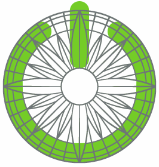
\includegraphics[width=3.5cm]{images/TitlePage/Acte.png}
%\end{minipage}%
%\begin{minipage}[t]{0.23\linewidth}
%	\centering
%	
\includegraphics[width=3.5cm]{images/TitlePage/Micmac.png}
%\end{minipage}%
%\begin{minipage}[t]{0.23\linewidth}
%	\centering
%	
\includegraphics[width=3.5cm]{images/TitlePage/UPE.png}
%\end{minipage}%

	
%\noindent {\large \textbf{Université Gustave Eiffel}} \\
\vspace*{0.3cm}
\noindent {\LARGE \textbf{MSTIC Doctoral School}} \\
\noindent \textbf{Mathematics \& Sciences and Technologies\\of Information and Communication} \\
\vspace*{0.5cm}
\noindent \Huge \textbf{Ph.D Thesis} \\
\vspace*{0.3cm}
\noindent \large {to obtain the title of} \\
\vspace*{0.3cm}
%\noindent \LARGE \textbf{PhD of Science} \\
%\vspace*{0.3cm}
\noindent \Large Doctorate of the Gustave Eiffel University \\
%\noindent \Large \textbf{Specialty : \textsc{Computer Science}}\\
\vspace*{0.4cm}
\noindent \large {Defended by\\}
\noindent \huge Lulin \textsc{Zhang} \\
\vspace*{0.8cm}
\noindent {\Huge \textbf{Feature matching for multi-epoch historical aerial images}} \\
%quasi-nadir
%\noindent {\Huge \textbf{Supervised learning for interest points matching in archive/analogue and modern/digital images}} \\
\vspace*{0.8cm}
\noindent \Large Thesis Advisor: \\
Marc \textsc{Pierrot Deseilligny}, Ewelina \textsc{Rupnik}\\
\vspace*{0.2cm}
\noindent \Large prepared at Univ. Gustave Eiffel/Lastig ACTE/IGN/ENSG\\
\vspace*{0.2cm}
\noindent \large defended on May xx, 2022 \\
\vspace*{0.5cm}
\end{center}
\noindent \large \textbf{Jury :} \\
\begin{center}
%\noindent \large \textbf{Reviewer:} Marie-Odile Berger  INRIA Nancy\\
%\noindent \large \textbf{Reviewer:} El Mustapha Mouaddib\\
%\noindent \large \textbf{Examiner:} Denis Feurer\\
%\noindent \large \textbf{Examiner:} Livio De Luca\\
%\noindent \large \textbf{Invited Member:} Yann Klinger\\
%\noindent \large \textbf{Invited Member:} Michele Santangelo\\
\begin{tabular}{lr}
\textbf{Reviewer:} Marie-Odile Berger & INRIA Nancy\\
\textbf{Reviewer:} El Mustapha Mouaddib & UPJV\\
%Université de Picardie Jules Verne (UPJV)
\textbf{Examiner:} Denis Feurer & IRD\\
%Institut de recherche pour le développement (IRD)
\textbf{Examiner:} Livio De Luca & CNRS\\
\textbf{Invited Member:} Yann Klinger & IPGP\\
\textbf{Invited Member:} Michele Santangelo & CNR-IRPI\\
\end{tabular}

%\begin{tabular}{llcl}
%      \textit{Reviewers :}	& Patrick \textsc{Clarysse}		& - & CNRS (CREATIS)\\
%				& Louis \textsc{Collins}		& - & McGill University\\
%      \textit{Advisor :}	& Grégoire \textsc{Malandain}		& - & INRIA (Asclepios)\\
%      \textit{President :}	& Nicholas \textsc{Ayache}		& - & INRIA (Asclepios)\\
%      \textit{Examinators :}   & Pierre-Yves \textsc{Bondiau}          & - & Centre Antoine Lacassagne (Nice)\\
%      				& Guido \textsc{Gerig}			& - & University of North Carolina\\
%      				& Vincent \textsc{Grégoire}		& - & Université Catholique de Louvain\\
%      \textit{Invited :}		& Hanna \textsc{Kafrouni}		& - & DOSISoft S.A.
%\end{tabular}
\end{center}
\end{titlepage}

\pagenumbering{arabic}
\sloppy

\titlepage

\restoregeometry

\pagenumbering{roman}


\setcounter{page}{0}
\cleardoublepage

\section*{Acknowledgments}
%After nearly 3 years of research, I am about to finish my PhD career. Looking back on these years, tons of feelings well up in my mind, among them there are content, promising, stressful, determined, and most importantly grateful feelings. I am deeply grateful for the people and things I met.\\
%First of all, I would like to thank my supervisors Marc and Ewelina. They offered me this PhD position when I needed a new start in France, and I thank them for their recognition and trust in me. During my PhD, they gave me a lot of guidance and help in my work, I learned a lot from them. Marc is a senior specialist in photogrammetry, he possesses profound experience in this domain, from which I benefited a lot. He is like a steersman, very good at controlling the direction. Ewelina is versatile, she is there for me whenever I have a problem. She is capable of many unexpected skills that surprises me, both in algorithm and operation. More importantly, both of them are rigorous scholars, they set up role models for me in my future research.
%I'd also like to thank Yann Klinger and Institut de Physique du Globe de Paris who made this PhD position possible. 
%%sebastian, KAGAM for providing data
%\\
%Secondly, I would like to thank my husband, Teng Wu, who is also an academic in photogrammetry. He gave me a lot of useful advises in my work. He is also a very reliable partner in life, I got countless help and support from him. Although he is not very expressive, he is fully devoted to me and our family. I know that he will support me unconditionally whenever I need him, he met all the expectations I had for a life partner.\\
%Thanks to the gift of life, we have two healthy and lovely daughters who bring joy and hope into our lives. Since having them, we have a deeper sense of responsibility and a stronger motivation to become better examples for them.\\
%Besides, I am grateful to my parents for raising me and for supporting all the choices I made in my life. Thanks to my brother, who took over the responsibility of taking care of my parents for me after I left China. As an aged PhD student, it is not easy to balance work and life, I can't imagine pursuing my PhD without the support from all the family members I mentioned before.\\
%During my research at Lastig, I met many warm-hearted friends: Manchun, Yilin, Imane, Mohamed, Arthur, Christophe, Jean-Michael, Jean-Philippe, Lanfa, Nathan, Raphael, Evelyn etc., who made my work environment full of friendliness and laughter. I am grateful to all the friends in my life who enriched me and I look forward to meeting and talking with them more often after the covid is alleviated.

\dominitoc
\tableofcontents

%!TEX root = Manuscript.tex

\chapter*{List of Acronyms}
\mtcaddchapter[List of Acronyms]

% Define here acronyms used in the manuscript. Copy paster the example for each new acromnym you would like to use

%\begin{acronym}
%\renewcommand{\\}{}
%\newacronym{DSM}{DSM}{Digital Surface Model}
%%\acro{DTI}{Diffusion Tensor Imaging}
%\end{acronym}
%\acro{DSM}{Digital Surface Model}

\begin{acronym}
	\acro{GCP}[GCP]{Ground Control Point}
	\acro{DSM}[DSM]{Digital Surface Model}
	\acro{DoD}[DoD]{Difference of DSMs}
	\acro{GT}[GT]{Ground Truth}
	\acro{IGN}[IGN]{Institut national de l'information géographique et forestière}
	\acro{BBA}[BBA]{Block Bundle Adjustment}
\end{acronym}

%Abbreviations
%
%IGN
%IPGP
%Lastig
%ENSG
%
%intra-epoch: from the same time
%inter-epoch: from different times
%DSM: Digital Surface Model
%DoD: Difference of DSMs
%GCP: Ground Control Point
%BBA: Bundle block adjustment
%GSD: Ground sampling distance



\mainmatter

Abbreviations

IGN
IPGP
Lastig
ENSG

intra-epoch: from the same time
inter-epoch: from different times
DSM: Digital Surface Model
DoD: Difference of DSMs
GCP: Ground Control Point
BBA: Bundle block adjustment

%!TEX root = Manuscript.tex

%解释DSM,DoD,GCP,multi-epoch, intra and inter epoch, GT
\chapter{Introduction}
\label{chap:intro}
\minitoc

\section{Motivation}
\subsection{Why are historical images interesting}
Historical (i.e. analogue or archival) aerial images play an important role in providing unique information about evolution of land-covers. 
They are objective witness over time and sometimes the only remaining visual source of historical land-form. Therefore, they are valuable assets for a wide range of applications such as: (1) change detection, (2) spatial and urban planning, (3) long-term environmental monitoring including but not limited to forests, ice glaciers and coastlines, (4) analysis of natural disaster (e.g. earthquake, volcano eruption, landslide ect.) and the estimation of its future trends, etc.
%用途:地震,冰川,土地规划?
%long-term environmental monitoring: forests, ice glaciers, coastlines etc.
%change detection; 
%spatial and urban planning, boundary disputes, etc.
%enable the analysis of natural disaster (e.g. earthquake, volcano eruption, landslide ect.) and the estimation of its future trends.
\par
Historical aerial images have regularly been acquired since the 1920’s by mapping, military or cadastral agencies all over the world. A mass amount of them have been digitized and made accessible through web services~\cite{sebastien2019archiving,earthexplorer,remonterletemps}. 
For example, according to a survey in Europe~\cite{sebastien2019archiving}, there are in total 50 million of aerial images archived, with around 37.8\% of them digitized.
%A survey called "State of current practices concerning archival aerial images" in Europe~\cite{sebastien2019archiving} took place in 2017, 19 organizations from 13 countries (including Austria, Norway, Finland, Spain, Slovenia, Cyprus, Czech Republic, Finland, Germany, Switzerland, Sweden, Poland, France and United Kingdom) replied. According to it, there are in total 50 million of aerial images archived, with around 37.8\% of them digitized.
The images are of high spatial resolution, and are acquired in stereoscopic configuration, allowing for 3D restitution of territories. 
They are often accompanied by metadata, in most cases including the camera focal length and the physical sensor size. Other metadata such as flight plans, camera calibration certificates or orientations are not commonly available. 
\par
When the camera calibration parameters are unknown, they should be evaluated by a process called self-calibrating bundle adjustment. Adequate Ground Control Points (GCPs) are required, otherwise inaccurately estimated camera parameters will lead to systematic error surfaces called dome effect (i.e. bowel effect).
Generally, GCPs originate from (i) field surveys \cite{micheletti2015application,walstra2004time,cardenal2006use}, (ii) recent orthophotos and DEM \cite{nurminen2015automation,ellis2006measuring,fox2008unlocking} and (iii) recent satellite images \cite{ellis2006measuring,ford2013shoreline}. The most challenging part is to identify the GCPs on the historical images, due to inevitable scene changes. GCPs are usually manually measured with the help of recent photos, however, it is still monotonous and time-consuming. 
There is an urgent need to automatically identify corresponding points (i.e. matches) on historical and recent images.\\
When users are only interesting in comparing different historical epochs, the self-calibration can be accomplished without GCPs. Matches between different epochs would serve as observations in bundle adjustment to eliminate the dome effect between surfaces from different epochs. In conclusion, the bottleneck of historical image self-calibration located in recovering matches on images taken at different times (i.e. multi-epoch).
%困难:
%(1) 数据异构: images exhibit highly heterogeneous spatial resolutions, with very different acquisition conditions (season, sensors etc.); 
%(2) camera's parameters  may not be available as they might  be  lost  during  the  years  or  never documented; inappropriate film/glass plate preservation; deformation due to scanning process; 
%(3)Drastic scene changes
%(4)Low radiometric quality: old-fashioned radiometric characteristics; noisy; even scratchs on the original films; deterioration due to the aging of the film

%Corresponding points 
%Besides, inappropriate film/glass plate preservation and the scanning process enforce reestimating of the camera calibrations (i.e., the self-calibrating).\\

\subsection{How to match multi-epoch historical images}
However, matching multi-epoch historical images remains challenging, despite the fact that there exists a large number of image matching algorithms with their effectiveness proven on modern images, for the following reasons:
\begin{itemize}
	\item Multi-epoch images are often acquired at different times of day and in different weathers or seasons, which unavoidably leading to appearance differences.
	\item The scene changes over time due to anthropogenic phenomenas (e.g. urban planning) or natural ones (e.g. earthquake), especially for large time gaps.
	\item Multi-epoch images often exhibit heterogeneous spatial resolutions, accompanied with different acquisition conditions (sensors, spectral channels, etc.).
	\item Historical images are often facing low radiometric quality, including low contrast, image noise, deterioration due to the aging of the films, or even scratches on the films.
\end{itemize}
\subsubsection{Divide and conquer}
%分成CoReg和Precise,前者侧重robust,后者侧重精度.
\subsubsection{Take advantage of 3D geometry}
The key idea of our method is to use 3D geometry to guide matching. This idea comes from the observation that RGB images have the following shortcomings:\\
(1) Their appearances change over time (see Figure~\ref{AppearanceChange}), and with varying view angles on non-Lambertian surfaces (see Figure~\ref{PoorlyTextured}).\\
(2) Self similarities (e.g. repetitive patterns) favor false matches (see Figure~\ref{PoorlyTextured}).\\

\begin{figure*}[htbp]
	\begin{center}
		\subfigure[Image 1971]{
			\begin{minipage}[t]{0.45\linewidth}
				\centering
				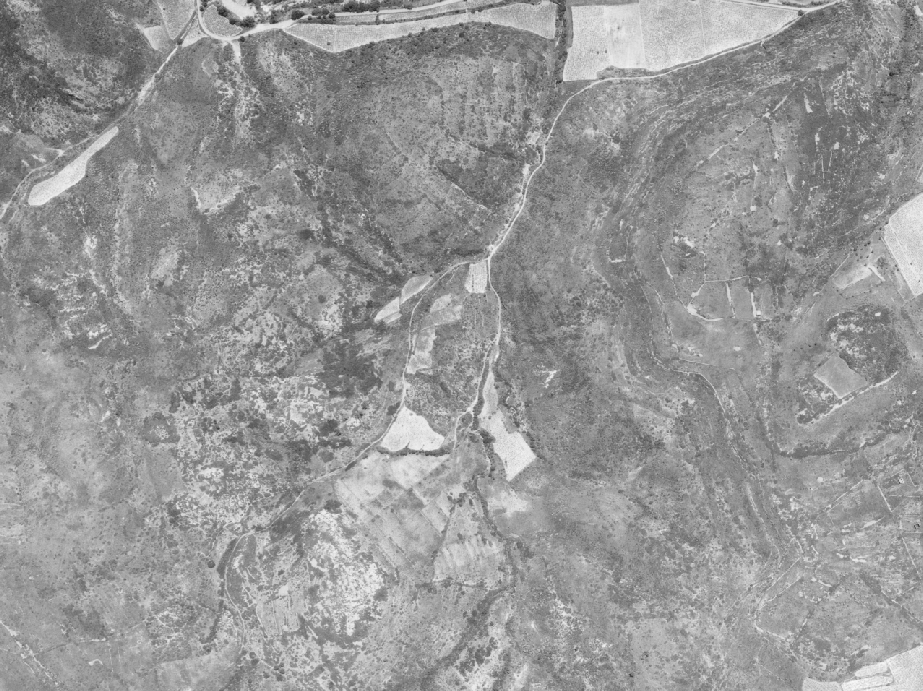
\includegraphics[width=6.2cm]{images/Chapitre1/AppearanceChangeRGBL.png}
			\end{minipage}%
		}
		\subfigure[Image 2015]{
			\begin{minipage}[t]{0.45\linewidth}
				\centering
				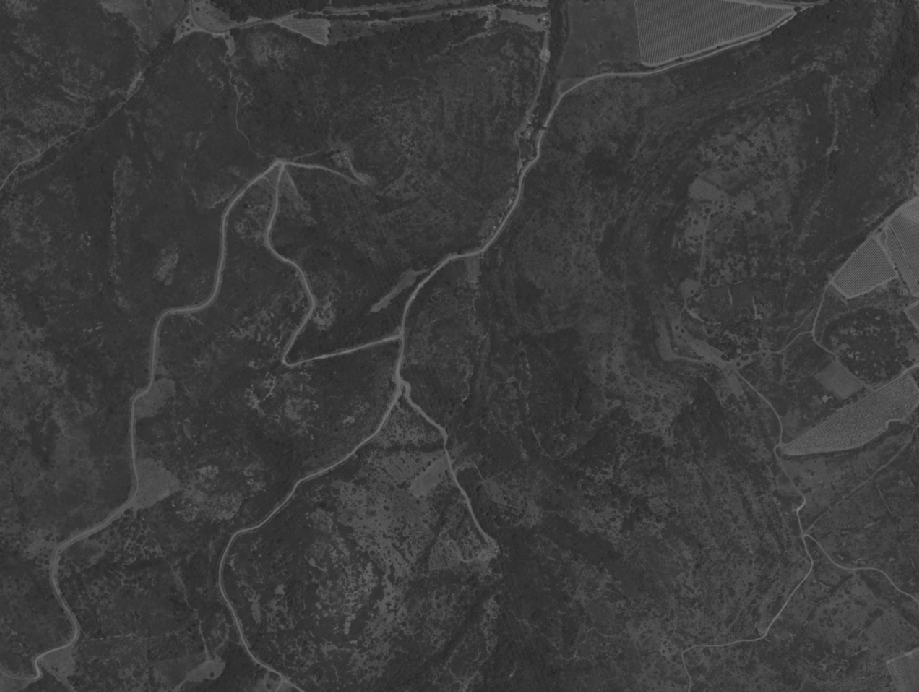
\includegraphics[width=6.2cm]{images/Chapitre1/AppearanceChangeRGBR.png}
			\end{minipage}%
		}
		\subfigure[DSM 1971]{
			\begin{minipage}[t]{0.45\linewidth}
				\centering
				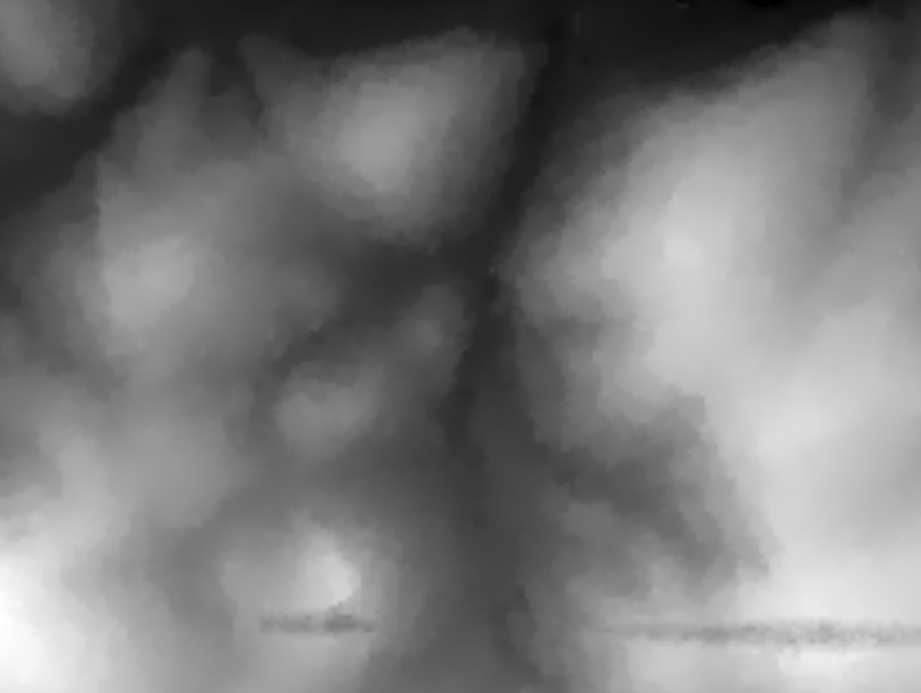
\includegraphics[width=6.2cm]{images/Chapitre1/AppearanceChangeDSML.png}
			\end{minipage}%
		}
		\subfigure[DSM 2015]{
			\begin{minipage}[t]{0.45\linewidth}
				\centering
				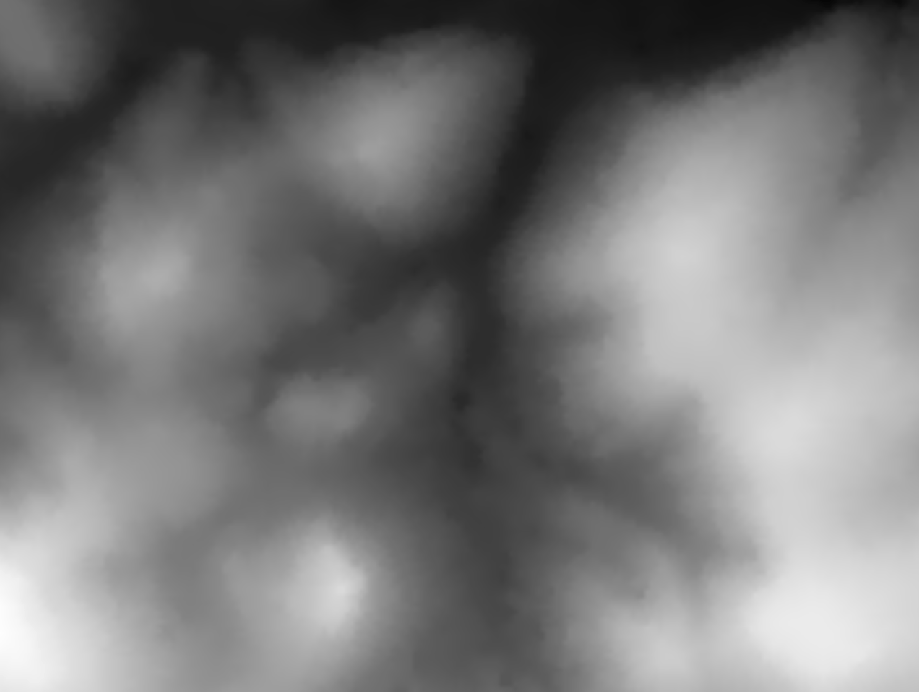
\includegraphics[width=6.2cm]{images/Chapitre1/AppearanceChangeDSMR.png}
			\end{minipage}%
		}
		\caption{The same zone observed in different times. The images changed a lot while the DSMs stayed stable over time.}
		\label{AppearanceChange}
	\end{center}
\end{figure*} 


\begin{figure*}[htbp]
	\begin{center}
		\subfigure[Image 1971]{
			\begin{minipage}[t]{0.45\linewidth}
				\centering
				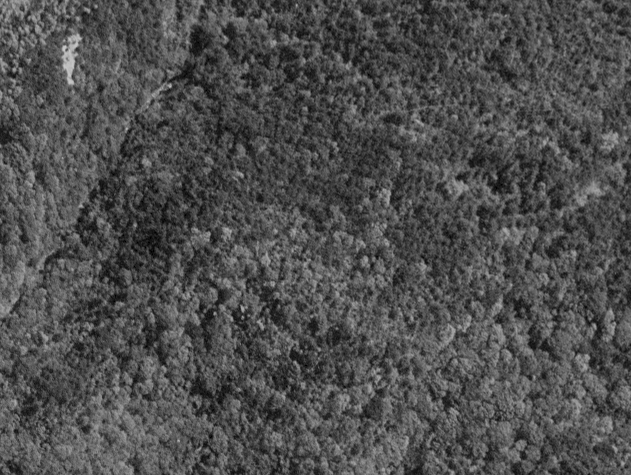
\includegraphics[width=6.2cm]{images/Chapitre1/PoorlyTexturedRGBL.png}
			\end{minipage}%
		}
		\subfigure[Image 2015]{
			\begin{minipage}[t]{0.45\linewidth}
				\centering
				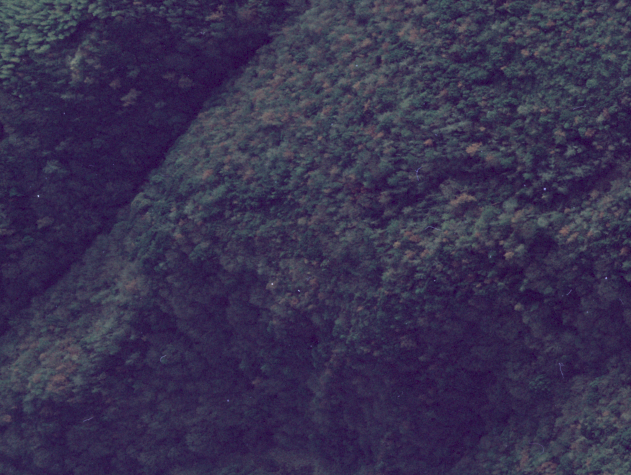
\includegraphics[width=6.2cm]{images/Chapitre1/PoorlyTexturedRGBR.png}
			\end{minipage}%
		}
		\subfigure[DSM 1971]{
			\begin{minipage}[t]{0.45\linewidth}
				\centering
				
\includegraphics[width=6.2cm]{images/Chapitre1/PoorlyTexturedDSML.png}
			\end{minipage}%
		}
		\subfigure[DSM 2015]{
			\begin{minipage}[t]{0.45\linewidth}
				\centering
				
\includegraphics[width=6.2cm]{images/Chapitre1/PoorlyTexturedDSMR.png}
			\end{minipage}%
		}
		\caption{The same vegetation observed in different times. They present non-Lambertian reflection and self similarities, while the DSMs are distinctive.}
		\label{PoorlyTextured}
	\end{center}
\end{figure*} 

\section{Objective}

\section{Contribution}

\section{Organization of the thesis}


%!TEX root = Manuscript.tex

\chapter{Literature review}
\label{chap:intro}
\minitoc

\section{Local feature matching}
Local feature refers to finding a discriminative structure found in an image, such as a point, corner, blob, edge or image patch. It is often accompanied with a descriptor, which is a compact vector representing the local neighborhood.
\par
According to the different data storage types, descriptors can be divided into two categories: floating-point descriptors and binary descriptors. The former is recorded in floating-point format, which has the advantage of being informative. It is widely used in various matching scenarios.
The latter is stored in binary type, which guarantees faster processing while demanding less memory. It is particularly suitable for real-time and/or smartphone applications.
Since our goal is to match multi-epoch images for high accuracy ground survey, we are interested in floating-point descriptors rather than binary ones.
\par
According to whether machine learning techniques are applied, local features can be categorized as hand-crafted or learned. We will subsequently elaborate on the two categories of approaches.
\subsection{Hand-crafted methods}
In the early stage, Moravec detects corner feature by measuring the sum-of-squared-differences (SSD) by applying a small shift in a number of directions to the patch around a candidate feature \cite{moravec1980obstacle}. Based on this, Harris computes an approximation to the second derivative of the SSD with respect to the shift \cite{harris1988combined}. Since both Moravec and Harris are sensitive to changes in image scale, algorithms invariant to scale and affine transformations based on Harris are presented \cite{mikolajczyk2004scale}. Other than corner feature, SIFT (Scale-invariant feature transform) \cite{lowe2004distinctive} detects blob feature in scale-space, which is an entire pipeline including detection and description. It uses a difference-of-Gaussian function to identify potential feature points that are invariant to scale and orientation. SIFT is a milestone among hand-crafted features, and comparable with machine learning alternatives. RootSIFT \cite{arandjelovic2012three} uses a square root (Hellinger) kernel instead of the standard Euclidean distance to measure the similarity between SIFT descriptors, which leads to a dramatic performance boost. Similar to SIFT, SURF \cite{bay2006surf} resorts to integral images and Haar filters to extract blob feature in a computationally efficient way. DAISY \cite{tola2009daisy} is a local image descriptor, which uses convolutions of gradients in specific directions with several Gaussian filters to make it very efficient to extract dense descriptors. KAZE \cite{alcantarilla2012kaze} is an algorithm that detects and describes multi-scale 2D feature in nonlinear scale spaces. AKAZE \cite{Alcantarilla13bmvc} is an accelerated version based on KAZE.
\subsection{Learned methods}
With the rise of machine learning, learned features have shown their feasibility in the image matching problem when enough ground truth data is available. 
FAST \cite{rosten2006machine} uses decision tree to speed up the process of finding corner feature. 
LIFT (Learned Invariant Feature Transform) \cite{yi2016lift} is a deep network architecture that implements a full pipeline including detection, orientation estimation and feature description. It is based on the previous work TILDE \cite{verdie2015tilde}, the method of \cite{moo2016learning} and DeepDesc \cite{simo2015discriminative}. 
Tian et al. introduced L2-Net~\cite{tian2017l2} to learn high performance descriptor in Euclidean space via the Convolutional Neural Network (CNN). 
Afterwards Mishchuk et al.~\cite{mishchuk2017working} introduced a compact descriptor named HardNet, by applying a novel loss to L2Net \cite{tian2017l2}. 
DELF \cite{noh2017DELF} is an attentive local feature descriptor based on CNN, which works particularly well for illumination changes.
SuperPoint \cite{detone2018superpoint} is a self-supervised, fully-convolutional model that operates on full-sized images and jointly computes pixel-level feature point locations and associated descriptors in one forward pass. 
LF-Net \cite{ono2018lf} is a deep architecture that embeds the entire feature extraction pipeline, and can be trained end-to-end with just a collection of images. 
D2-Net \cite{dusmanu2019d2} is a single neural network that works as a \textit{dense} feature descriptor and a feature detector simultaneously, but their keypoints are less accurate compared to classical features since they are extracted on feature maps which have a resolution of 1/4 of the input resolution.
ASLFeat~\cite{luo2020aslfeat} improves shape-awareness and localization accuracy by applying light-weight yet effective modifications on an improved D2-Net.
R2D2 \cite{revaud2019r2d2} is a CNN architecture that learns \textit{dense} local descriptors (one for each pixel) as well as two associated repeatability and reliability confidence maps.
Contextdesc ~\cite{luo2019contextdesc} is a unified learning framework that leverages and aggregates the cross-modality contextual information.
D2D \cite{wiles2020d2d} allows \textit{dense} features to be modified based on the differences between the images by conditioning the feature maps on both images. 
Different than the aforementioned feature extraction methods, SuperGlue \cite{sarlin2020superglue} presents a new way of thinking about the feature matching problem. 
%Instead of learning better task-agnostic local features followed by simple matching heuristics and tricks, SuperGlue
%It learns the matching process from pre-existing local features 
It matches two sets of pre-existing local features by adopting a flexible context aggregation mechanism based on attention to jointly find correspondences and reject non-matchable points.
\par
Early learned methods (LIFT ~\cite{yi2016lift}, L2-Net~\cite{tian2017l2}, HardNet~\cite{mishchuk2017working}, DELF ~\cite{noh2017DELF}, SuperPoint ~\cite{detone2018superpoint}, LF-Net ~\cite{ono2018lf}) use only intermediate metrics (e.g., repeatability, matching score, mean matching accuracy, etc.) to evaluate the matching performance. 
Even though they demonstrate better performance when compared to hand-crafted features on certain benchmark, it does not necessarily imply a better performance in terms of subsequent processing steps. For example, in the context of Structure from Motion (SfM), finding additional correspondences for image pairs where SIFT already provides enough matches does not necessarily results in more accurate or complete reconstructions \cite{schonberger2017comparative}.
Jin et al.~\cite{jin2020image} introduced a comprehensive benchmark for local features and robust estimation algorithms, focusing on the accuracy of the reconstructed camera pose as the primary metric. Using the new metric, SIFT ~\cite{lowe2004distinctive} and SuperGlue ~\cite{sarlin2020superglue} take the lead~\cite{imagematchingchallenge2020}.

\section{Historical image processing}
%\subsection{General processing pipeline}
%Archiving and geoprocessing of historical aerial images: current status in europe,official publication no 70. European Spatial Data Research~\cite{sebastien2019archiving}
%\subsection{Inter-epoch historical images alignment}
When it comes to inter-epoch historical images, however, directly applying SIFT or SuperGlue often results in inferior results due to large radiometric differences.
In Figure~\ref{comparison} we showed an example where SIFT and SuperGlue failed on an inter-epoch image pair with drastic scene changes. It is understandable as (1) SIFT is not sufficiently invariant over time, while (2) SuperGlue is not invariant to rotations and it underperforms on larger images because it was presumably trained on small images.\\
Therefore, many previous researches bypassed the task of extracting inter-epoch correspondences by processing different epochs separately followed by an inter-epoch co-registration relying on Ground Control Points(GCPs).
Between 10 and 169 GCPs are required in ~\cite{pinto2019archived}, ~\cite{bozek2019analysis}, ~\cite{persia2020archival}, ~\cite{micheletti2015application}, ~\cite{molg2017structure}.
GCPs are usually measured with the help of photointerpretation on recent orthophotos, however, it is still monotonous and time-consuming. Furthermore, it is difficult to find salient points that are stable over time.\\
Certain attempts were made to extract inter-epoch correspondences. Giordano et al.~\cite{giordano2018toward} extract feature correspondences between historical and recent images relying on HoG descriptors~\cite{dalal2005histograms}. The authors require flight plans as input, which are not commonly available as mentioned in Section 1. Feurer et al.~\cite{feurer2018joining}, Filhol et al.~\cite{filhol2019time}, Cook et al.~\cite{cook2019simple}, Parente et al.~\cite{parente2021automated} and Blanch et al.~\cite{blanch2021multi} assume that a sufficient number of keypoints remain invariant across time and employ SIFT to extract inter-epoch feature correspondences. It remains questionable whether the method is capable of handling drastic scene changes.
Zhang et al.~\cite{zhang2020guided} extract inter-epoch correspondences from SIFT-detected keypoints based on the hypothesis that points follow 2D and 3D spatial similarity model. This method works in simple cases with few scene changes.
{Additionally, a stream of research works focuses on historical terrestrial images (~\cite{maiwald2021automatic}, ~\cite{beltrami20193d}, ~\cite{bevilacqua2019reconstruction}, ~\cite{maiwald2019generation}) and historical video recordings (~\cite{maiwald2019generation}). However, their algorithms are not suitable to the aerial case.}\\
This work is an extention of~\cite{zhang2020guided}. Unlike in~\cite{zhang2020guided}, we introduce a rough co-registration between different epochs based on matching DSMs with SuperGlue, and use it to guide a precise matching. Our rough co-registration is robust under extreme scene changes because (1) SuperGlue utilizes context to enhance feature descriptors and (2) DSMs are generally stable over time. With the guidance of roughly co-registered orientations and DSMs, both SIFT and SuperGlue achieved good performance, as shown in our experiments.
\section{Robust matching}
The goal of robust matching is to tell apart inliers from outliers, and eliminate the latter from further processing.
\par
Typically, an iterative sampling strategy based on RANSAC (Random Sample Consensus) \cite{fischler1981random} relying on some mathematical model, such as homography \cite{sonka2014image} or essential matrix \cite{sonka2014image} is carried out to remove outliers. 
This is an important issue which was often not given sufficient attention.
LMedS (Least Median of Squares) \cite{leroy1987robust} is a meaningful groundwork before RANSAC, which is also commonly used to replace RANSAC.
MLESAC (Maximum Likelihood SAC)  \cite{torr2000mlesac} adopts the same sampling strategy as RANSAC but chooses the solution that maximizes the likelihood instead of the number of inliers. PROSAC (Progressive Sample Consensus ) \cite{chum2005matching} chooses samples from progressively larger sets of top-ranked correspondences, which makes it significantly faster than RANSAC. DEGENSAC \cite{chum2005two} is an algorithm for epipolar geometry estimation unaffected by planar degeneracy. It is widely used in the 2020 image matching challenge \cite{imagematchingchallenge2020}.
USAC (Universal RANSAC) \cite{raguram2012usac} framework is a synthesis of the various optimizations and improvements that have been proposed to RANSAC.
GC-RANSAC (Graph-Cut RANSAC) \cite{barath2018graph} runs graph-cut algorithm in the local optimization step.
MAGSAC \cite{barath2019magsac} eliminates the need for a user-defined inlier-outlier threshold with marginalization.
\par
Various deep learning methods have also been developed to handle the erroneous matches.
DSAC (the differentiable counterpart of RANSAC) \cite{brachmann2017dsac} replaces the deterministic hypothesis selection by a probabilistic selection.
CNe (Context Networks) \cite{moo2018learning} trains deep networks in an end-to-end fashion to label the correspondences as inliers or outliers, known intrinsics are required as input, and a post-processing with RANSAC is often tasked. CNe was embedded into the framework of \cite{jin2020image} to remove outliers, paired with DEGENSAC, PyRANSAC (a variant of DEGENSAC by disabling the degeneracy check, introduced in \cite{jin2020image}) and MAGSAC. The results showed that with SIFT used to train CNe, about 80\% of the outliers were filtered out. Nearly all classical methods benefited from CNe, but not the learned ones. Jin et al. \cite{jin2020image} also stated that RANSAC should be tuned to particular feature detector and descriptor, and specific settings should be selected for a particular RANSAC variant.
\par
In this research, we use RANSAC to estimate the 3D Helmert transformation between surfaces (i.e., DSMs) calculated in different epochs. Compared to the classical essential/fundamental matrix filtering, with less data (3 versus 5 points) we impose stricter rules on the sets of points. Lastly, we eliminate the remaining false correspondences by looking at their cross-correlation.


%!TEX root = Manuscript.tex

\chapter{Rough co-registration}
\label{chap:intro}
\minitoc

\section{Introduction}
The goal of rough co-registration is establishing a transformation model between different epochs to narrow down the search space in the subsequent precise matching step. It plays a fundamental role as wrong transformation model would lead to deviation from the right search space. Therefore robustness is the most critical target. In the meantime, it doesn't need to be very accurate as the precision would be improved in the precise matching part via searching the neighborhood.
\par
Generally, each inter-epoch image pair would be matched, followed by a RANSAC routine to recover the best transformation model.
%It is about getting reliable matches rather than obtaining accurately localized ones. 
Minimum matches between different epochs are required, depending on the model type:\\
\begin{enumerate}
    \item \textbf{2D similarity }transformation model, which requires at least 2 matches for each inter-epoch image pair to solve 4 parameters;
    \item \textbf{Homography }transformation model, which requires at least 4 matches for each inter-epoch image pair to solve 8 parameters;
    \item \textbf{3D Helmert }transformation model, which requires at least 3 matches for the whole block to solve 7 parameters.
\end{enumerate}
%The most critical target is to get reliable matches, instead of obtaining accurately localized ones.
%
Since multi-epoch images often demonstrate different appearances due to scene changes and heterogeneous acquisition conditions, we come up with 2 ideas to improve the matching robustness:\\
\begin{enumerate}
    \item Instead of building transformation models (2D similarity or homography) for each inter-epoch image pair that might contradict each other, it is better to build a 3D Helmert transformation model which is globally consistent over the whole block.
    \item Take 3D geometry into consideration to boost the matching performance.
\end{enumerate}
Based on these ideas, we attempted 2 strategies for multi-epoch rough co-registration:\\
\begin{enumerate}
    \item \textit{ImgPairs}: Match every possible combination of inter-epoch image pairs, followed by projecting the matches onto ground to build globally consistent transformation model.
    \item \textit{Ortho} or \textit{DSM}: (1) Generate orthophoto or DSM for each epoch; (2) match orthophoto or DSM pairs, followed by RANSAC based on 2D similarity transformation model to remove outliers; (3) project inlier mathces onto ground to build a 3D Helmert transformation model between epochs. 
\end{enumerate}

Our main contributions include:\\
\begin{enumerate}
	\item Improve matching robustness by building globally consistent transformation model, which can be achieved by either (1) matching each inter-epoch image pair followed by global filtering or (2) integrating images from the same epoch into a single image (DSM or orthophoto) before matching.
	\item Introduce the idea of matching DSMs to obtain robust matches even under drastic scene changes, as the 3D landscape often stays globally stable over time.
	\item Introduce RANSAC based on 3D Helmert transformation model for \textit{ImgPairs}: each three matches projected to DSM serve to compute a 3D Helmert transformation between epochs, and most importantly provide a 2D constraint on all images’ matches.
	\item Introduce \textit{4 rotation hypotheses} to make SuperGlue, which is not invariant to rotation larger than 45$^\circ$, practicable on remote sensing images.
	\item Introduce \textit{one-to-many tiling scheme} to scale-up the deep learning methods for feature matching.
	\item Improve the performance of matching inter-epoch images with SIFT by (1) using downsampled images and (2) skipping ratio test.% and FIGNN.
\end{enumerate}


%\subsection{Motivation}
%\subsection{Contribution}

\section{Methodology}
%Our goal is to improve robustness by building globally consistent transformation model over the whole block.
%In order to achieve this goal, we exploded 2 strategies:
%(1) matching each potential image pair followed with global filtering based on 3D RANSAC;\\
%(2) get a global image for each epoch first (DSM or orthophoto), apply matching and 2D RANSAC.\\
%零碎匹配,整体inlier
%整体匹配
%Our methods aim at roughly co-register 2 epochs to the same frame. One epoch (generally the more recent epoch) would be chosen as the reference epoch $E_r$, the other one would be treated as free epoch $E_f$. A transformation model would be built to move epoch $E_f$ to the frame of epoch $E_r$.\\
We provide 2 strategies for inter-epoch rough co-registration: matching image pairs (\textit{ImgPairs}) or matching orthophotos/DSMs (\textit{Ortho} and \textit{DSM}). The pipelines will be elaborated in the following sections. Please notice our pipelines are generic, different feature matching methods can be readily applied in them. At present we use either SIFT or SuperGlue to test our pipeline as they are currently \textit{state-of-the-art}, but they can be replaced when better matching methods appear in the future.\\
Our methods are not only able to match aerial or satellite images, but also able to match mixed images. Aerial images are supposed to be accompanied with focal lengths and physical sensor sizes, which are usually available. For historical aerial images, they should be resampled to the geometry of the fiducial marks prior to processing. 
%For the sake of simplicity, only 2 epochs are present in our processing flows, however, it can be easily extended to more epochs.
\par
We adopt the following naming conventions:\\
\begin{enumerate}
    \item Images acquired in \textit{epoch$_1$} and \textit{epoch$_2$} are denoted as $I^{e_1}$ and $I^{e_2}$;
    \item Orientations of \textit{epoch$_1$} and \textit{epoch$_2$} are denoted as $O^{e_1}$ and $O^{e_2}$; 
    %\item Ground extent of \textit{epoch$_1$} and \textit{epoch$_2$} are denoted as $G^{e_1}$ and $G^{e_2}$;
    \item Orthophotos of \textit{epoch$_1$} and \textit{epoch$_2$} are denoted as $Op^{e_1}$ and $Op^{e_2}$; 
    \item DSMs of \textit{epoch$_1$} and \textit{epoch$_2$} are denoted as $D^{e_1}$ and $D^{e_2}$.
\end{enumerate}
Before inter-epoch rough co-registration, we process each epoch individually to recover the relative orientations and DSM within the same epoch. It is a standard photogrammetry or SfM pipeline and can be accomplished with lots of solutions (e.g. MicMac~\cite{deseilligny2011apero}, COLMAP~\cite{schonberger2016structure}, {OpenMVG~\cite{openMVG}, Theia~\cite{theia}, etc.}). The solution used in our experiment is MicMac. It is performed within each \textit{epoch$_i$} individually as follows:
\begin{enumerate}
\item Extract intra-epoch matches between images $I^{e_i}$ with SIFT ~\cite{lowe2004distinctive};
\item Based on the sequential SfM to compute interior and relative orientations ({$O_{ini}^{e_i}$}) for aerial images, or to refine the RPC(Rational Polynomial Coefficient) for satellite images;
\item Based on image orientations $O_{ini}^{e_i}$, perform semi-global dense matching~\cite{mpd:06:sgm} {between images $I^{e_i}$} to get {DSM ($D_{ini}^{e_i}$) in their arbitrary coordinate frames.}
\item Orthorectify the images to get orthophotos ($Op_{ini}^{e_i}$) if the matching orthophotos strategic is applied.
%\item Project the images onto mean elevation plane ($G_{ini}^{e_i}$) get orthophotos ($Op_{ini}^{e_i}$).
\end{enumerate}
%Please notice that the step (1) and (2) would not be necessary if the epoch is satellite, since the orientations would be provided by RPC(Rational Polynomial Coefficient).\\
%Two different strategies are provided to perform the rough co-registration. The pipelines will be elaborated in the following sections. 
\subsection{Strategy 1: Matching image pairs (\textit{ImgPairs})}
%\subsection{Strategy 1: global filtering}
%CoReg-R3D
This method is for co-registering aerial epochs only. It is not practical for satellite epoch as they are often with large size and will decrease efficiency remarkably.\\
The workflow of matching image pairs strategy is displayed in Figure~\ref{WorkflowImgPair}(a).\\
We introduce \textit{4 rotation hypotheses} when feature matching method that is not invariant to rotations lager than 45$^\circ$ (e.g. SuperGlue) is applied.\\
The \textit{4 rotation hypotheses} works as follows (cf. Figure~\ref{WorkflowImgPair}(b)): 
\begin{enumerate}
    \item Rotate the secondary image by 90$^{\circ}$ four times;
    \item Match each rotated image with the master image;
    \item Keep the rotation hypothesis with most numerous matches.
\end{enumerate}
The \textit{4 rotation hypotheses} would not be applied when rotation invariant matching method (e.g. SIFT) is adopted.
\par
Assuming the numbers of images in \textit{epoch$_1$} and \textit{epoch$_2$} are P and Q individually, the strategy \textit{ImgPairs} works as follows:\\
\begin{enumerate}
    \item Match P$\times$Q image pairs respectively (with or without \textit{4 rotation hypotheses}, depending on whether the matching method is rotation invariant), giving rise to P$\times$Q sets of matches $M({\mathbf{K}^{e_1},\mathbf{K}^{e_2}})$ ($\mathbf{K}^{e_i}$ represents keypoints in image $I^{e_i}$).
    \item Run RANSAC based on 2D similarity transformation model for each image pair, giving rise to P$\times$Q sets of matches $M({\mathbf{\widetilde{K}}^{e_1},\mathbf{\widetilde{K}}^{e_2}})$ ($\mathbf{\widetilde{K}}^{e_i}$ represents keypoints in image $I^{e_i}$). This step aims to filter matches into a reasonable number, otherwise the subsequent global filtering would become prohibitive. (This step would be skipped if matching methods that simultaneously performed filtering during the matching procedure (e.g. SuperGlue) are applied in the previous step.)
    \item Project $\mathbf{\widetilde{K}}^{e_i}$ in the matches $M({\mathbf{\widetilde{K}}^{e_1},\mathbf{\widetilde{K}}^{e_2}})$ onto ground with the help of orientations $O_{ini}^{e_i}$ and DSM $D_{ini}^{e_i}$ individually, resulting in points on ground $\mathbf{KG}^{e_i}$.
    \item Sample matches $M({\mathbf{KG}^{e_1},\mathbf{KG}^{e_2}})$ iteratively to compute the 3D Helmert transformation RANSAC model:
\begin{equation}
\left [ \begin{array}{c}
{KG}_x^{e_2}\\
{KG}_y^{e_2}\\
{KG}_z^{e_2}
\end{array}
\right ] =\lambda \cdot \mathbf{R} \cdot {\left [ \begin{array}{c}
    {KG}_x^{e_1}\\
    {KG}_y^{e_1}\\
    {KG}_z^{e_1}
    \end{array}
    \right ]} + \left [ \begin{array}{c}
\Delta_x\\
\Delta_y\\
\Delta_z
\end{array}
\right ]. \label{eq:2DSim}
\end{equation}
    
%   \begin{equation*}
%       {KG_i^{e_2}} = \lambda \cdot \mathbf{R} \cdot {KG_i^{e_1}} + \mathbf{T} , \quad i \in [1,3] \label{eq:3Dsim}
%   \end{equation*}
where $\lambda$ is the scale factor, $\mathbf{R}$ is the rotation matrix and $\left [ \begin{array}{c}
    \Delta_x, \Delta_y, \Delta_z
\end{array}
\right ]$ $^{^T}$ is the translation vector.
We set the number of RANSAC iterations to 1000, and consider matches within $T_r$ of its predicted position as inliers. In our experiment, {$T_r$ was set to 50m.}
    % to find the best 3D Helmert transformation model.
\end{enumerate}

\begin{figure*}[htbp]
    \begin{center}
        \subfigure[Workflow of \textit{ImgPairs}]{
    \begin{minipage}[t]{1\linewidth}
        \centering
        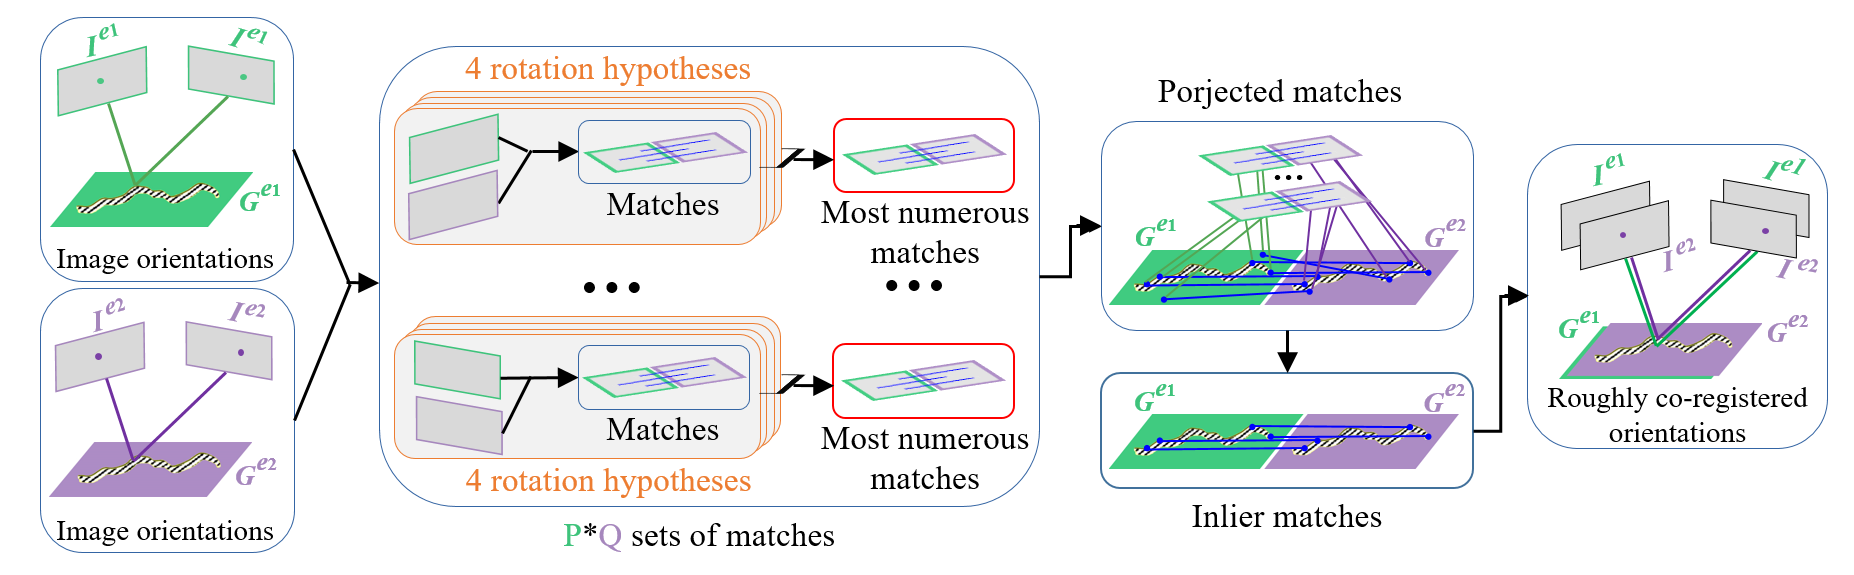
\includegraphics[width=1\columnwidth]{images/Chapitre3/R3D.png}
    \end{minipage}%
}
        \subfigure[Four rotation hypotheses]{
    \begin{minipage}[t]{0.8\linewidth}
        \centering
        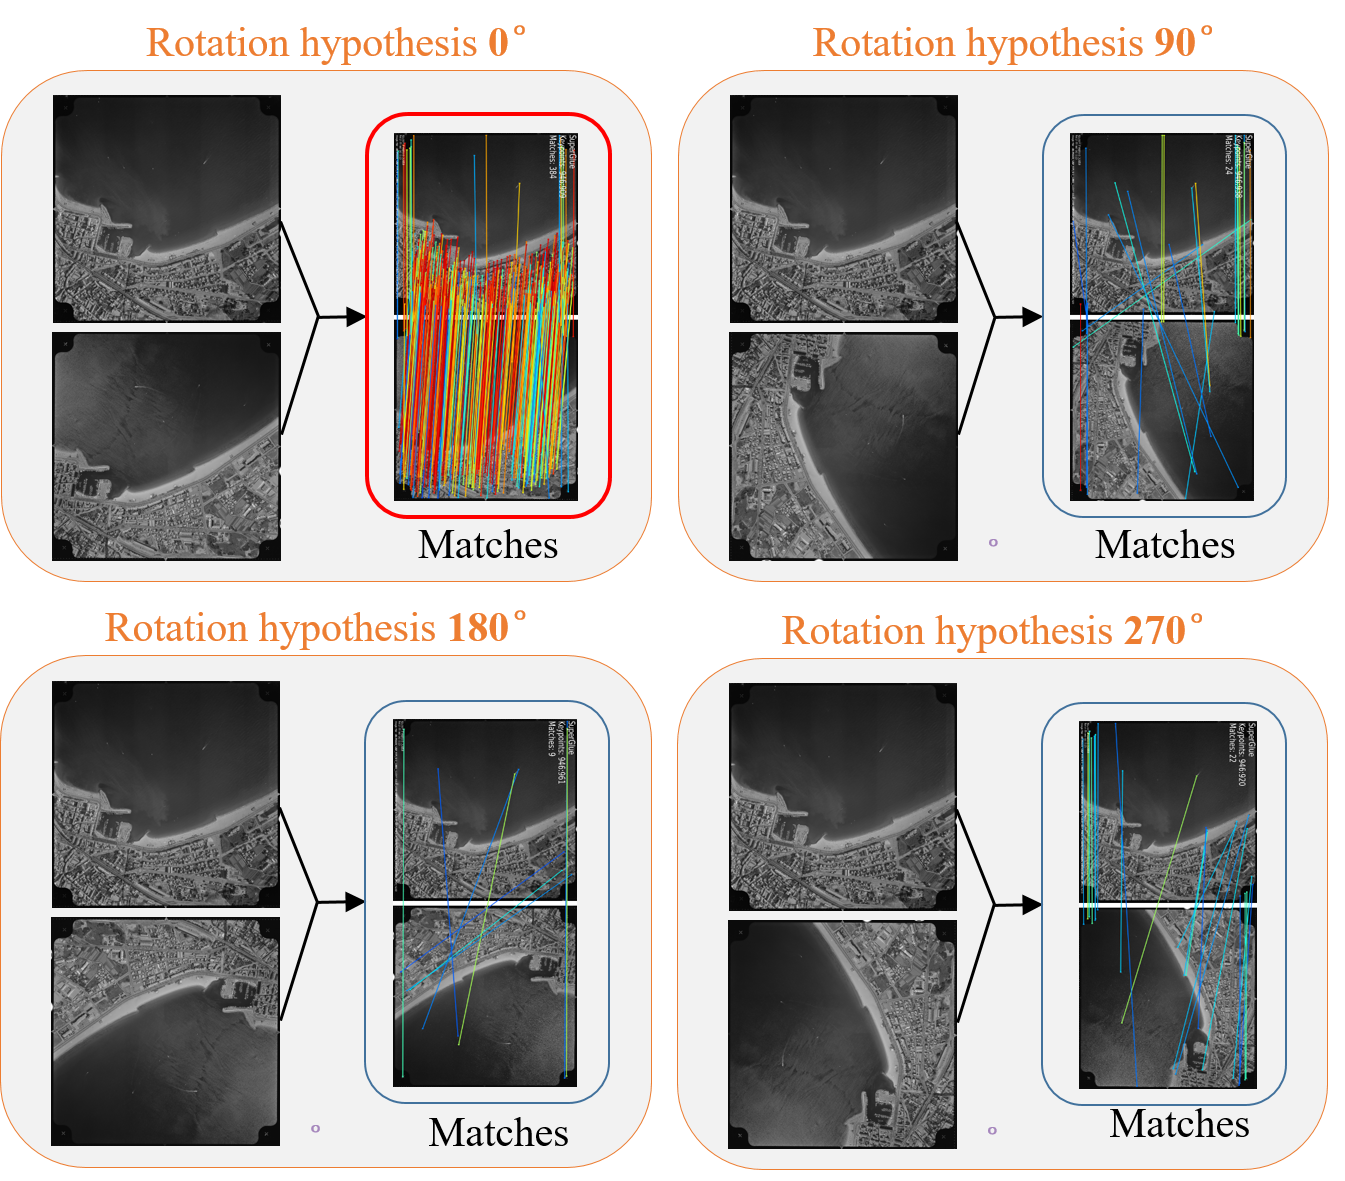
\includegraphics[width=0.8\columnwidth]{images/Chapitre3/R3D-RotHyp.png}
    \end{minipage}%
}
        \caption{Rough co-registration by matching image pairs. (a) Workflow of \textit{ImgPairs}. Each inter-epoch image pair is matched (with 4 rotation hypotheses which are explained in (b), if the matching method is not rotation invariant), followed by projecting the matches onto ground to find the globally consistent inliers. (b) Four rotation hypotheses. We rotate the secondary image by 90 $^\circ$ four times to match with master image and keep the best one with most numerous matches (red rectangle).}
        \label{WorkflowImgPair}
    \end{center}
\end{figure*}

This strategy is adapted from our early attempt to match different epochs by matching P$\times$Q inter-epoch image pairs individually without building a globally consistent transformation model. It is accomplished by estimating a 2D similarity model for each image pair in the first round of matching and using it to guide a second round of matching. Obviously it is less robust as the P$\times$Q 2D similarity models that should be consistent, might contradict each other.
\par
However, the idea of using 2D similarity model to guide matching is more generic as it doesn't require initial orientations $O_{ini}^{e_i}$ and DSMs $D_{ini}^{e_i}$. In Appendix ~\ref{chap:appendix3} we displayed images taken at the same time over an area covered with snow. It is extremely challenging to match them as very few useful context is available, both SIFT and SuperGlue failed on them. We provide the option to input a set of 2D similarity transformation parameters to narrow down the search space and therefore successfully recovered a large number of good matches. The 2D similarity transformation parameters can be estimated by manually measuring 2 matches. Even though it involves manual operation, the work load is negligible and worthy.
%helpful in specific cases when the orientations $O_{ini}^{e_i}$ and DSMs $D_{ini}^{e_i}$ are not available. This might happen when we don't have stereoscopic configuration  due to difficulty to match intra-epoch image pairs. In Appendix ~\ref{chap:appendix3} we displayed a small dataset over snow-covered area. It consists of only one epoch. However, there are images among them that are extremely challenging to match, both SIFT and SuperGlue failed on it. We provide the option to input a rough 2D similarity transformation model for prediction to narrow down the search space and therefore successfully recovered several good matches.

%\begin{figure*}[htbp]
%    \begin{center}
%        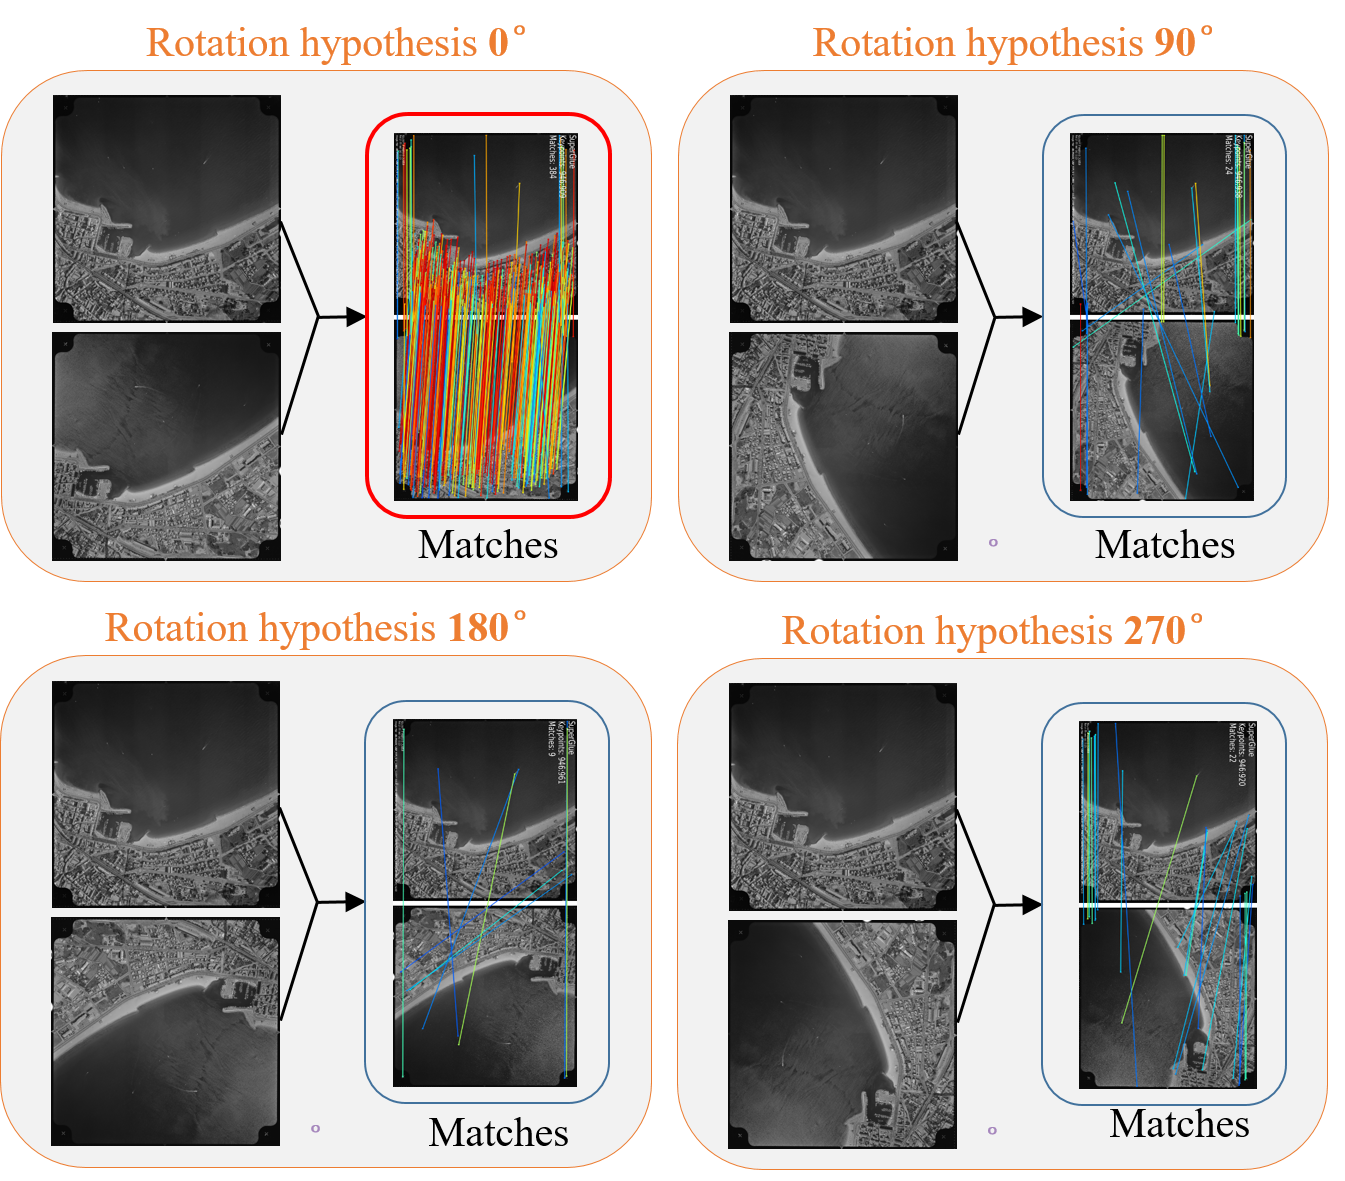
\includegraphics[width=0.8\columnwidth]{images/Chapitre3/R3D-RotHyp.png}
%        \caption{4 rotation hypotheses of matching image pairs.}
%        \label{Flow-process diagram}
%    \end{center}
%\end{figure*}

%\subsubsection{SIFT}
%\subsubsection{SuperGlue}
\subsection{Strategy 2: Matching Orthophotos/DSMs (\textit{Ortho} or \textit{DSM})}
%\subsection{trategy 2: global matching}
Another strategy is to match orthophotos or DSMs, which is suitable for both aerial images and satellite images. The workflows are displayed in Figure~\ref{WorkflowOrtho}(a) and Figure~\ref{WorkflowDSM}(a) individually. Different than matching P$\times$Q image pairs, we only need to match a pair of DSMs/orthophotos.
Orthophotos are by nature RGB images, therefore feature matching methods can be applied on them directly. Conversely, DSMs are 2.5D rasters recorded in floating-point format, they should be converted beforehand to [0–255] range grayscale images.
\par
\begin{figure*}[htbp]
    \begin{center}
        \subfigure[Workflow of \textit{Ortho}]{
            \begin{minipage}[t]{1\linewidth}
                \centering
                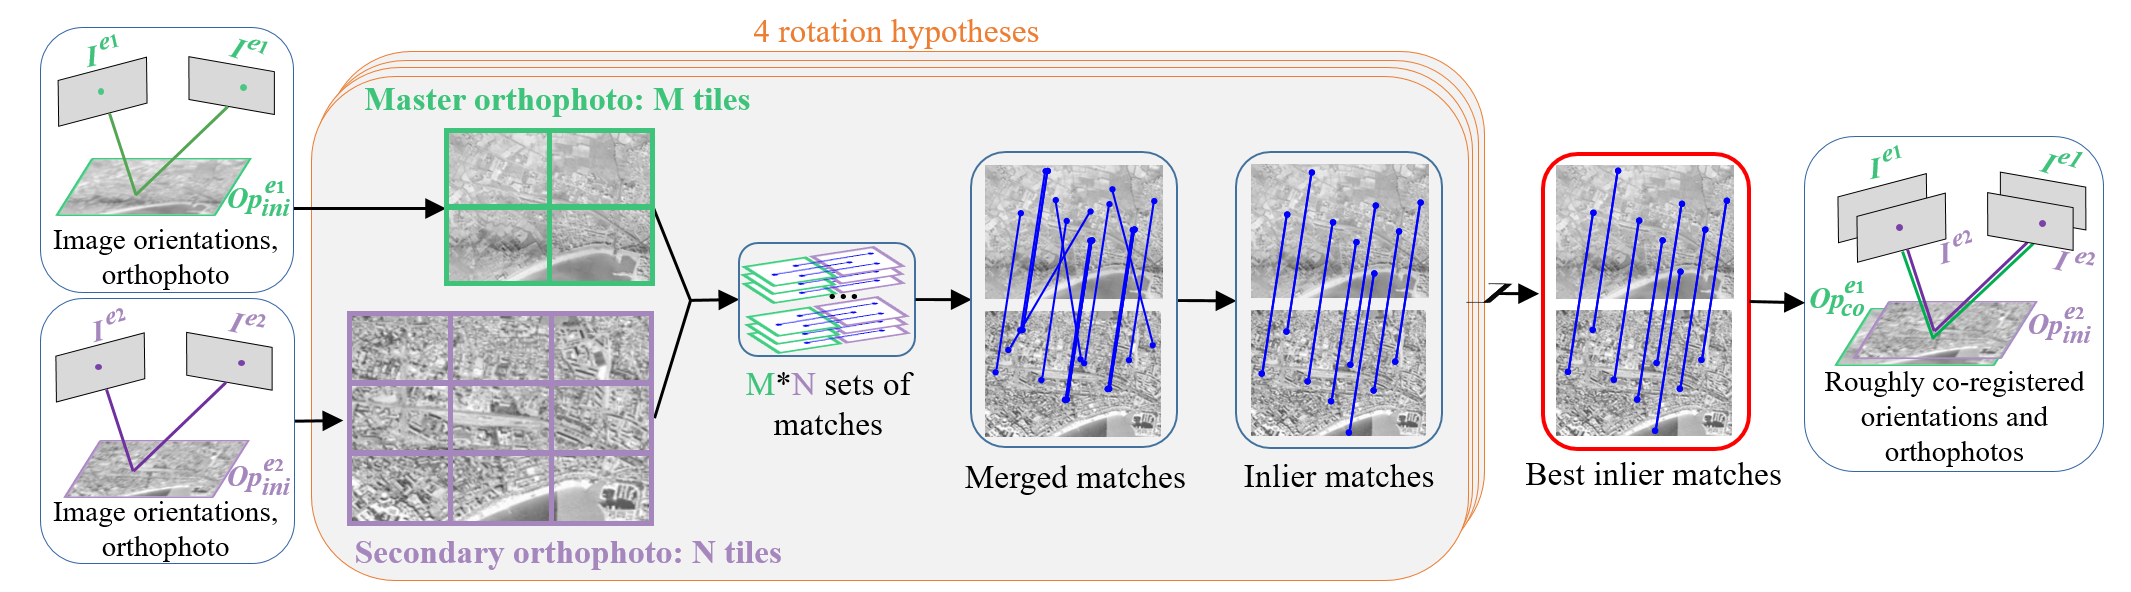
\includegraphics[width=1\columnwidth]{images/Chapitre3/ortho.png}
            \end{minipage}%
        }
        \subfigure[Four rotation hypotheses combined with \textit{one-to-many tiling scheme}]{
            \begin{minipage}[t]{1\linewidth}
                \centering
                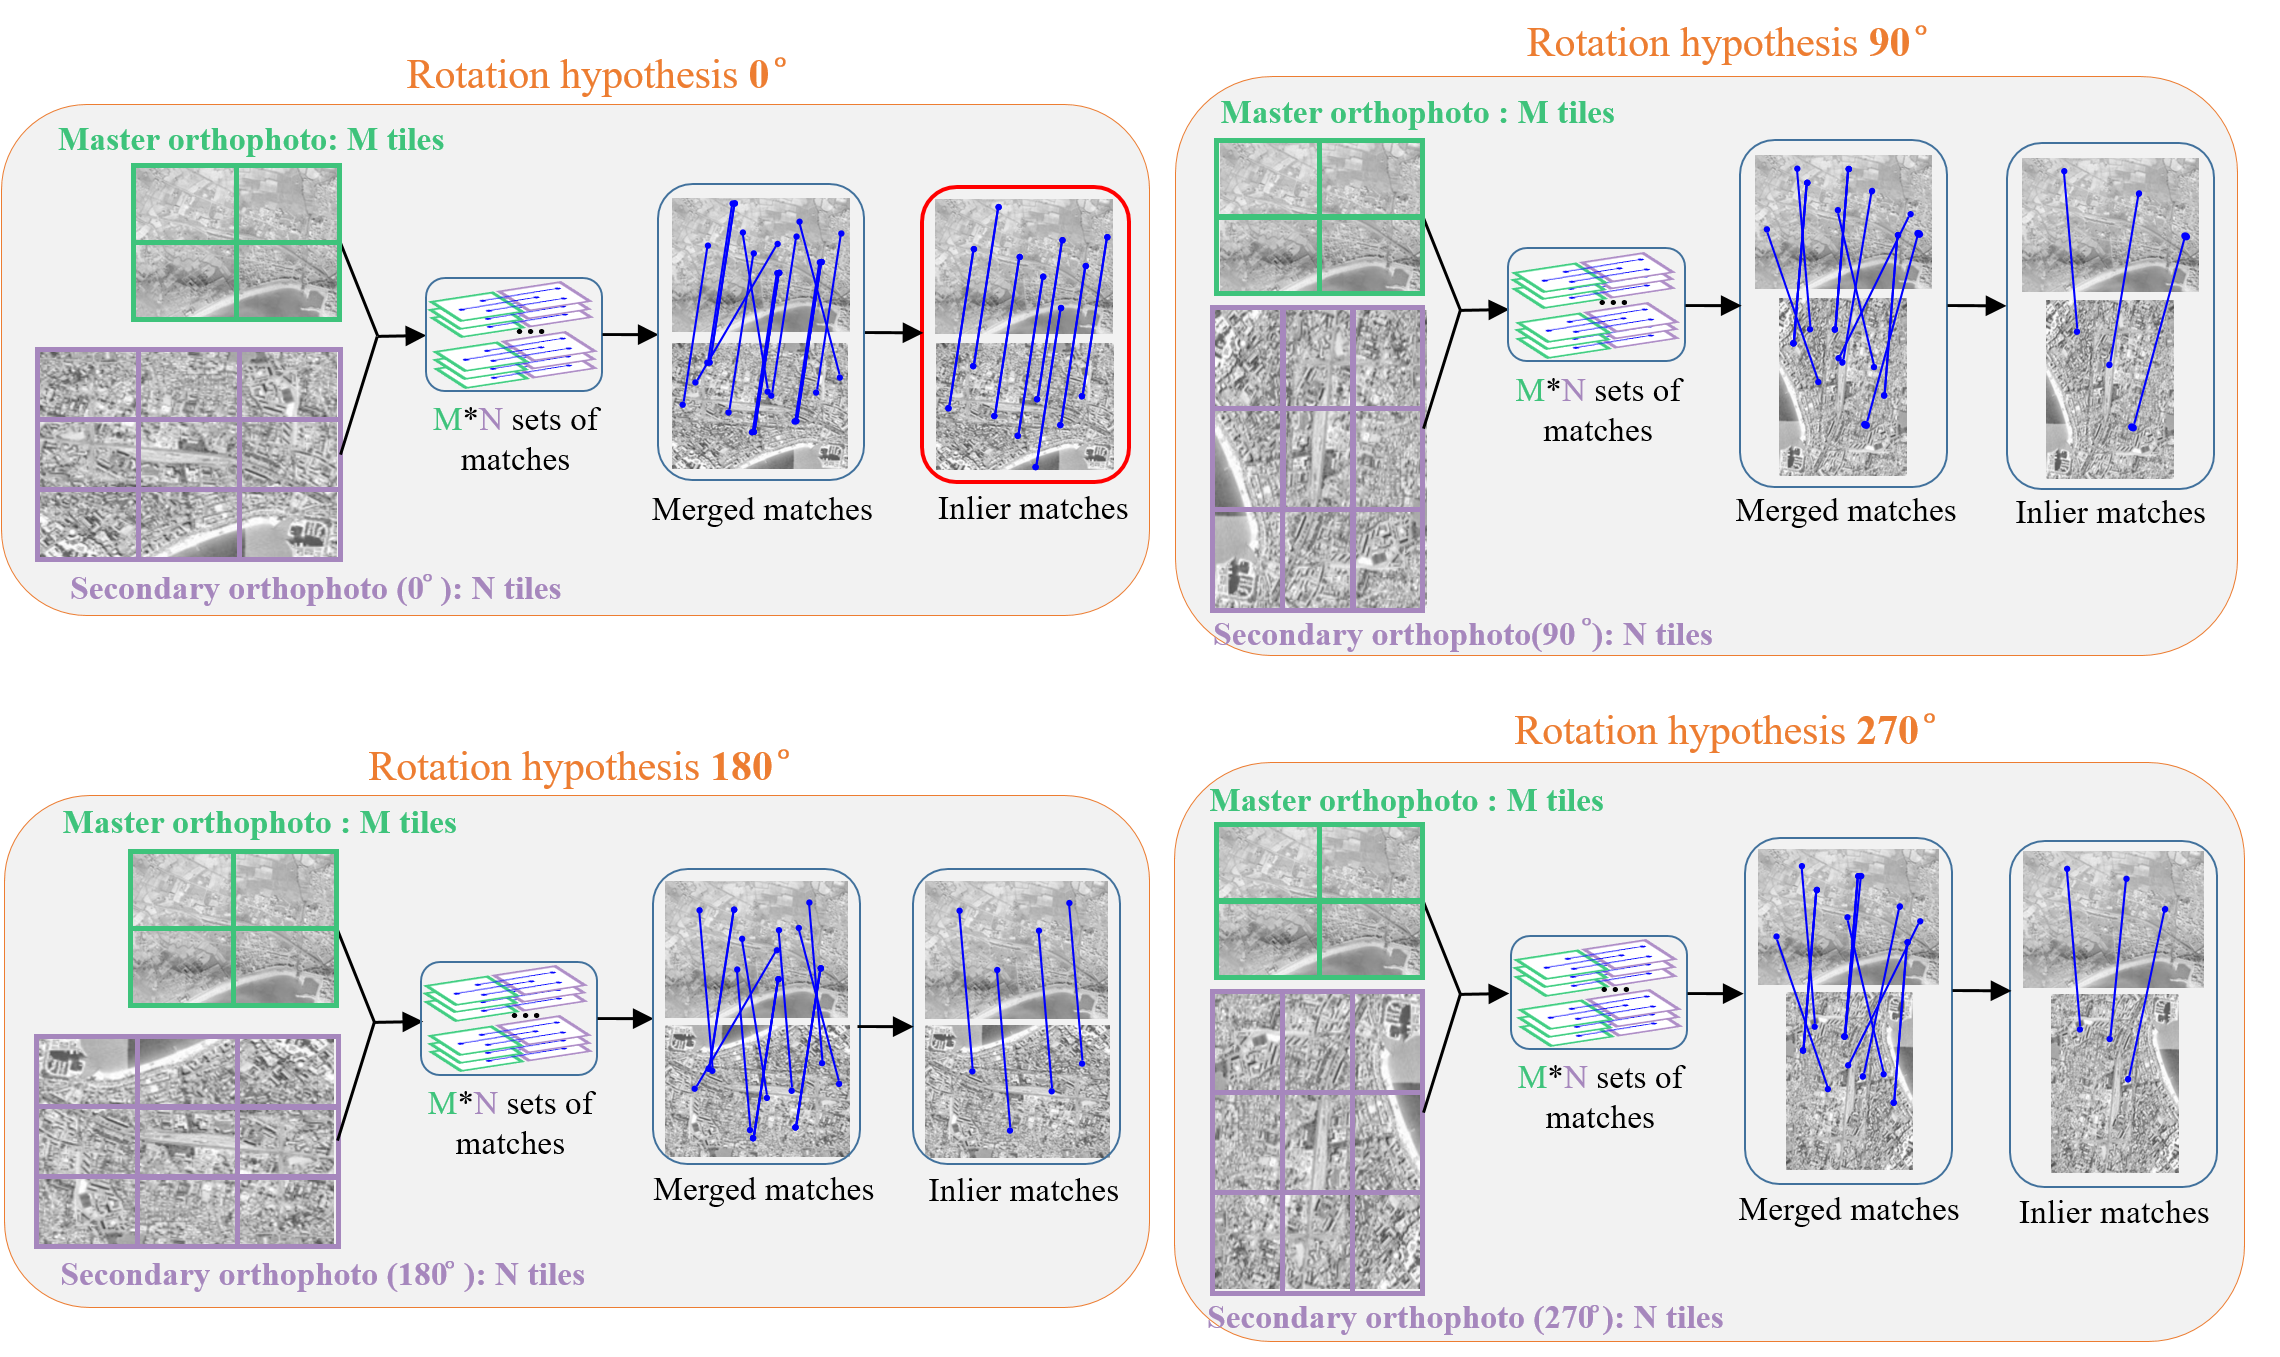
\includegraphics[width=1\columnwidth]{images/Chapitre3/ortho-RotHyp.png}
            \end{minipage}%
        }
        \caption{Rough co-registration by matching orthophotos. (a) Workflow of \textit{Ortho}. Orthophotos are matched (with \textit{one-to-many tiling scheme} combined with 4 rotation hypotheses which are explained in (b), if the matching method is unsatisfactory on large images and not rotation invariant), followed by projecting the inlier matches onto ground to build 3D Helmert transformation model. (b) Four rotation hypotheses combined with \textit{one-to-many tiling scheme}. We rotate the secondary orthophoto by 90 $^\circ$ four times to match with master orthophoto and keep the best one with most numerous RANSAC inliers (red rectangle). \textit{One-to-many tiling scheme} is applied during each hypothesis, with both orthophotos croped into tiles followed by matching all the tile pairs and merging the matches.}
        \label{WorkflowOrtho}
    \end{center}
\end{figure*}

%\begin{figure*}[htbp]
%    \begin{center}
%        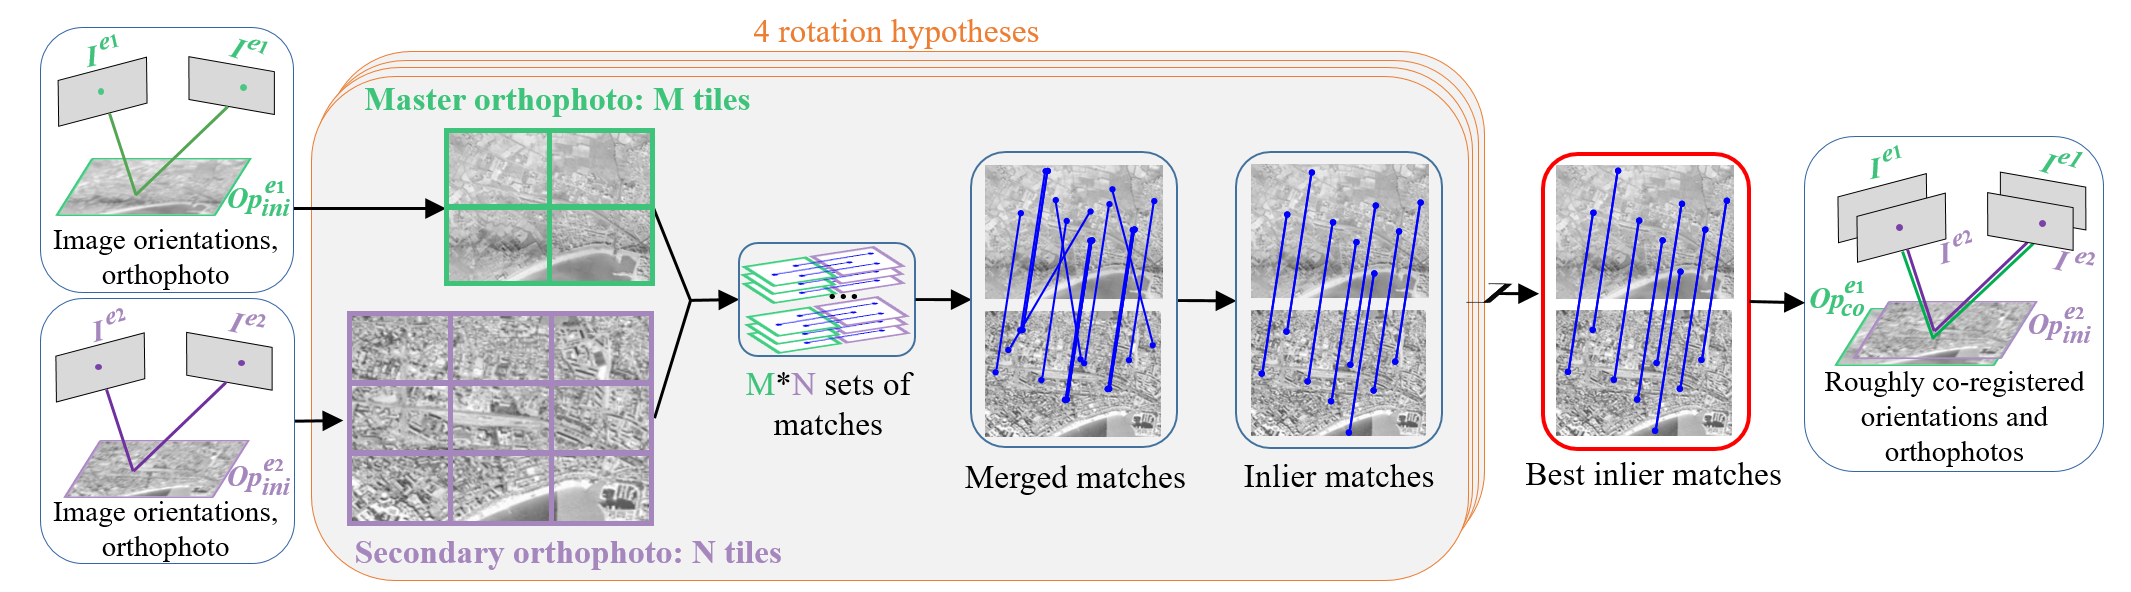
\includegraphics[width=1\columnwidth]{images/Chapitre3/ortho.png}
%        \caption{Rough co-registration by matching orthophotos.}
%        \label{Flow-process diagram}
%    \end{center}
%\end{figure*}
%
%\begin{figure*}[htbp]
%    \begin{center}
%        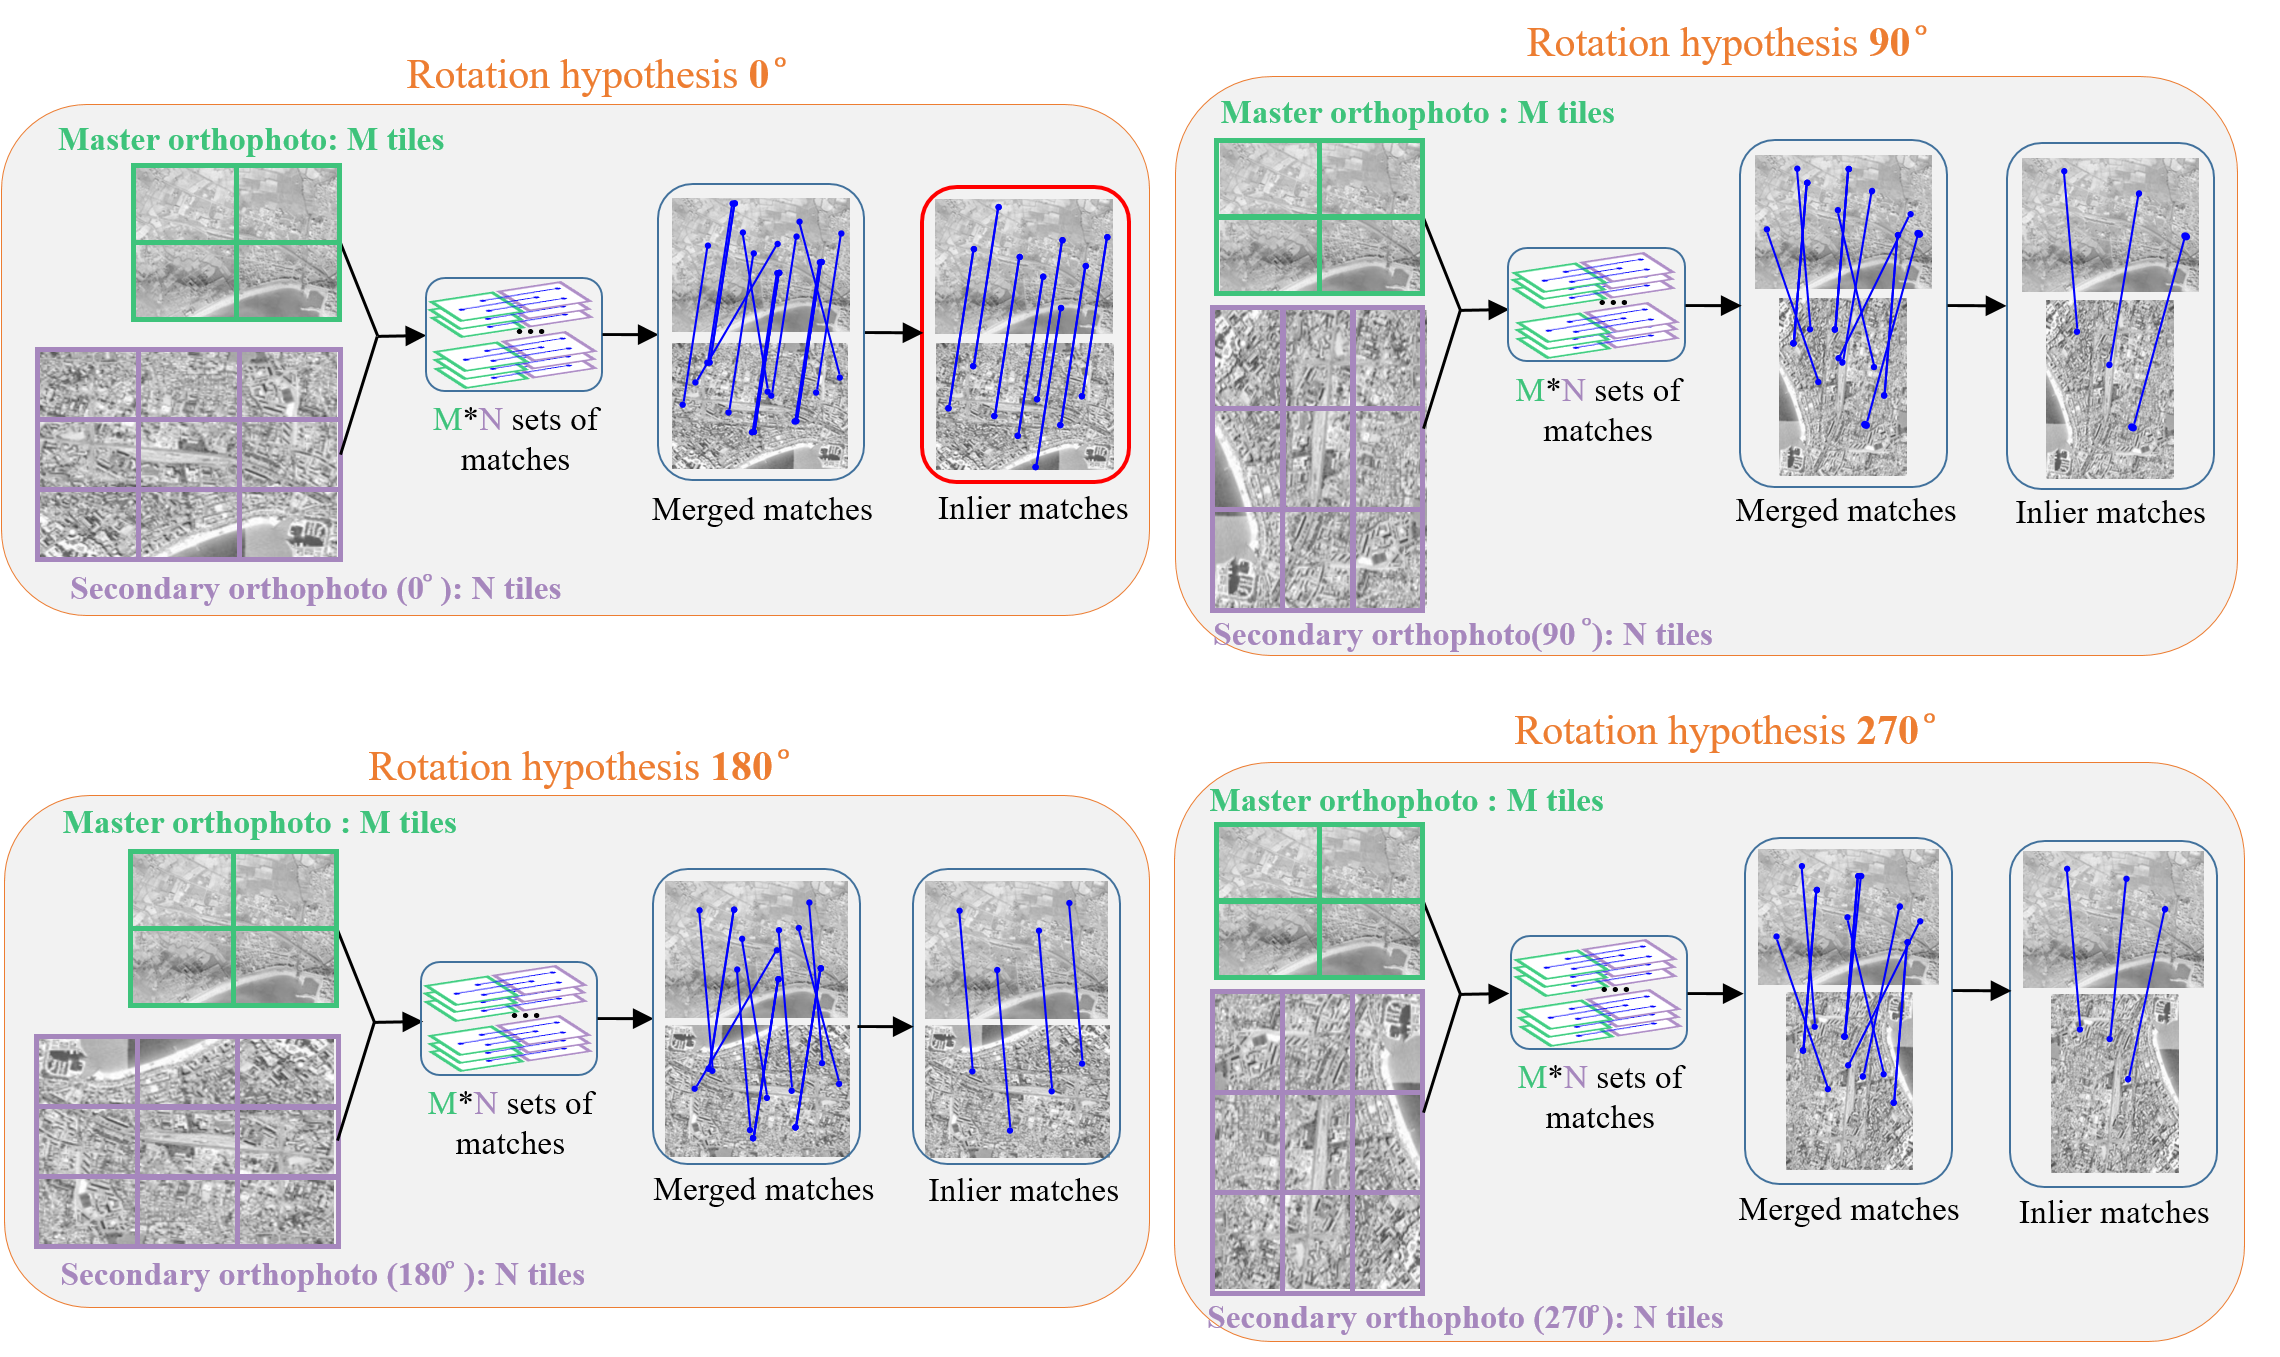
\includegraphics[width=0.8\columnwidth]{images/Chapitre3/ortho-RotHyp.png}
%        \caption{4 rotation hypotheses of matching orthophotos.}
%        \label{Flow-process diagram}
%    \end{center}
%\end{figure*}

%%%%%%%%%%%%%%%%%%%%%%%%%%%%%%

\begin{figure*}[htbp]
    \begin{center}
        \subfigure[Workflow of \textit{DSM}]{
            \begin{minipage}[t]{1\linewidth}
                \centering
                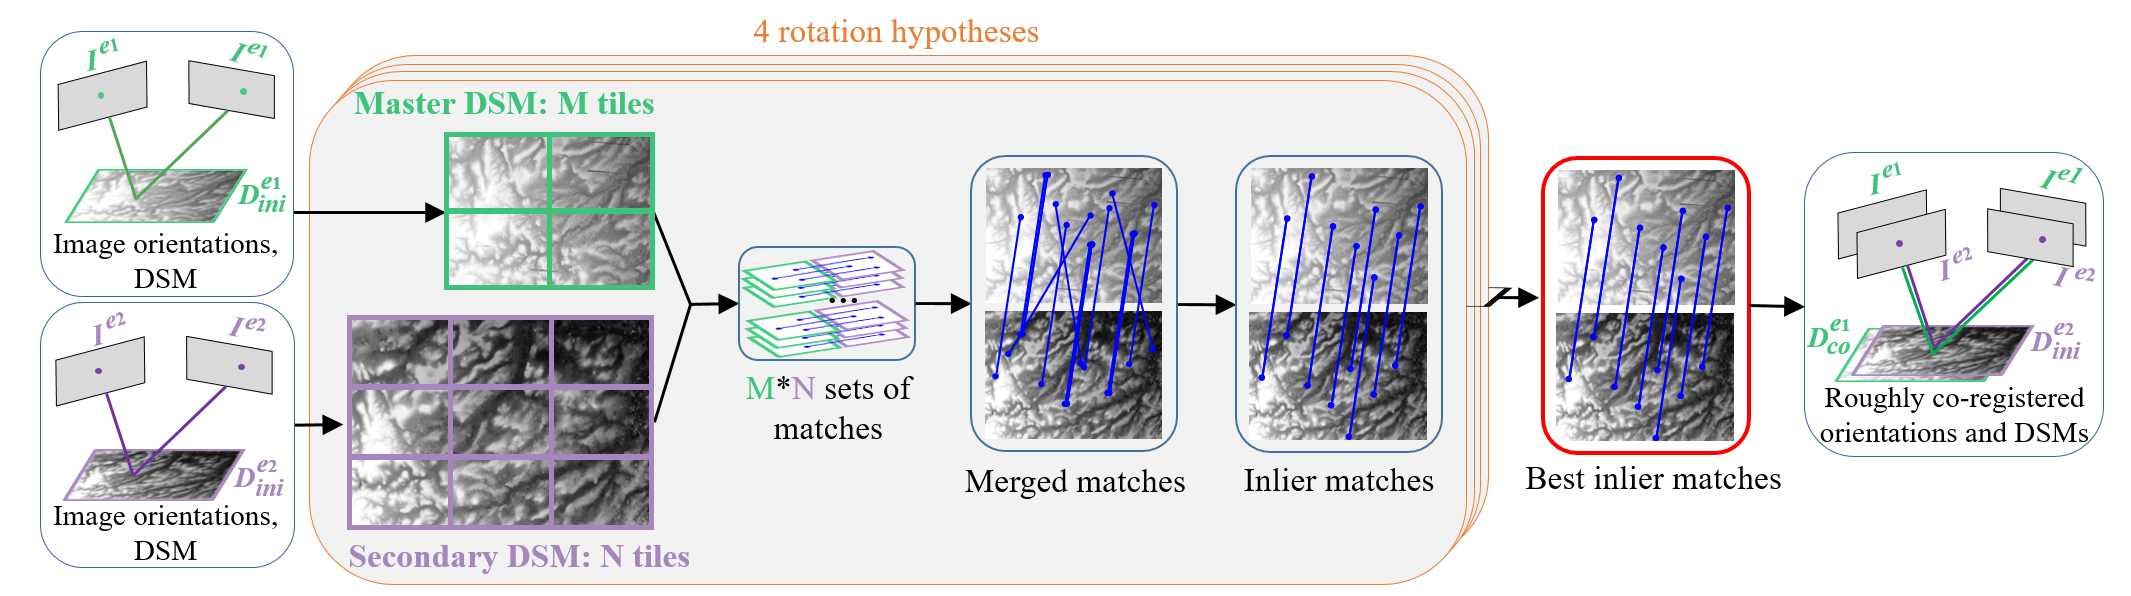
\includegraphics[width=1\columnwidth]{images/Chapitre3/dsm.png}
            \end{minipage}%
        }
        \subfigure[Four rotation hypotheses combined with tiling scheme]{
            \begin{minipage}[t]{1\linewidth}
                \centering
                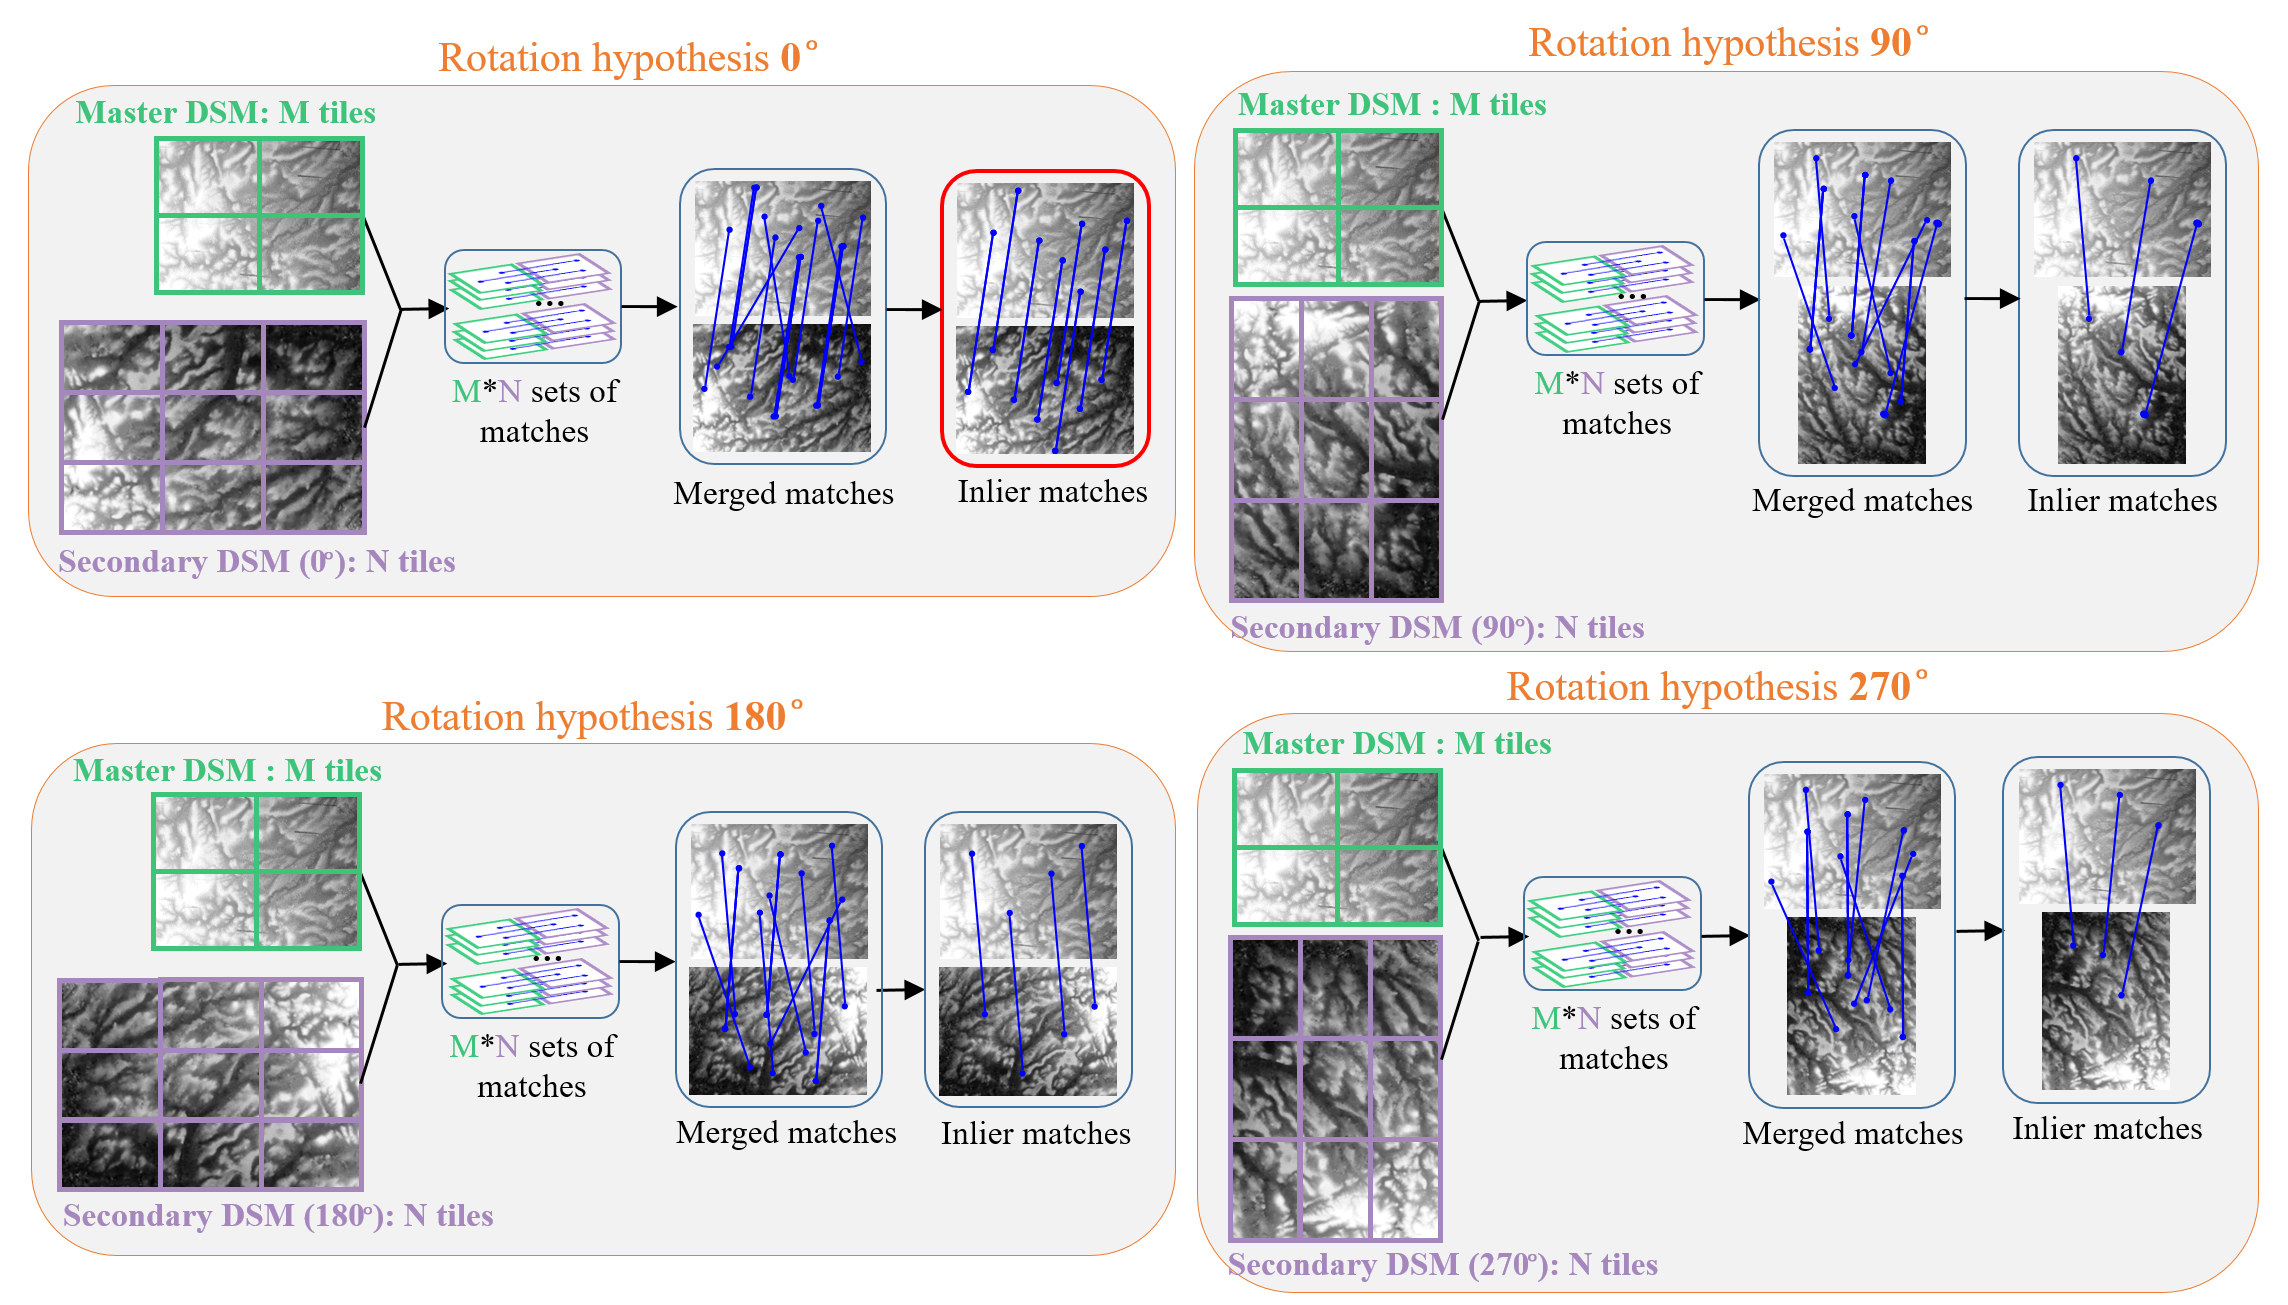
\includegraphics[width=1\columnwidth]{images/Chapitre3/dsm-RotHyp.png}
            \end{minipage}%
        }
        \caption{Rough co-registration by matching DSMs. (a) Workflow of \textit{DSM}. DSMs are matched (with \textit{one-to-many tiling scheme} combined with 4 rotation hypotheses which are explained in (b), if the matching method is unsatisfactory on large images and not rotation invariant), followed by projecting the inlier matches onto ground to build 3D Helmert transformation model. (b) Four rotation hypotheses combined with tiling scheme. We rotate the secondary DSM by 90 $^\circ$ four times to match with master DSM and keep the best one with most numerous RANSAC inliers (red rectangle). Tiling scheme is applied during each hypothesis, with both DSMs croped into tiles followed by matching all the tile pairs and merging the matches.}
        \label{WorkflowDSM}
    \end{center}
\end{figure*}

%\begin{figure*}[htbp]
%    \begin{center}
%        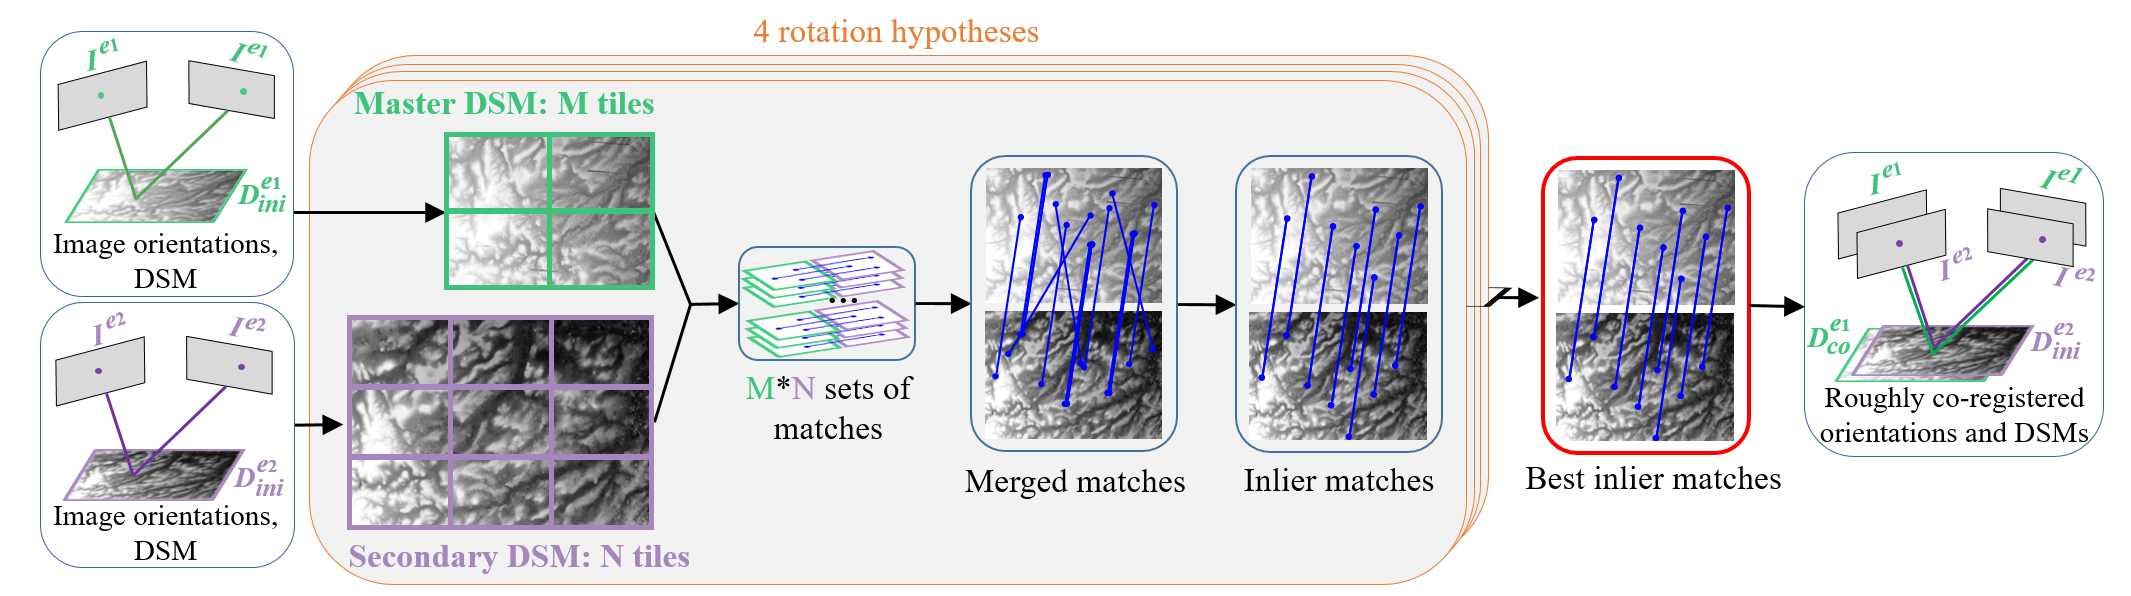
\includegraphics[width=1\columnwidth]{images/Chapitre3/dsm.png}
%        \caption{Rough co-registration by matching DSMs.}
%        \label{Flow-process diagram}
%    \end{center}
%\end{figure*}
%
%\begin{figure*}[htbp]
%    \begin{center}
%        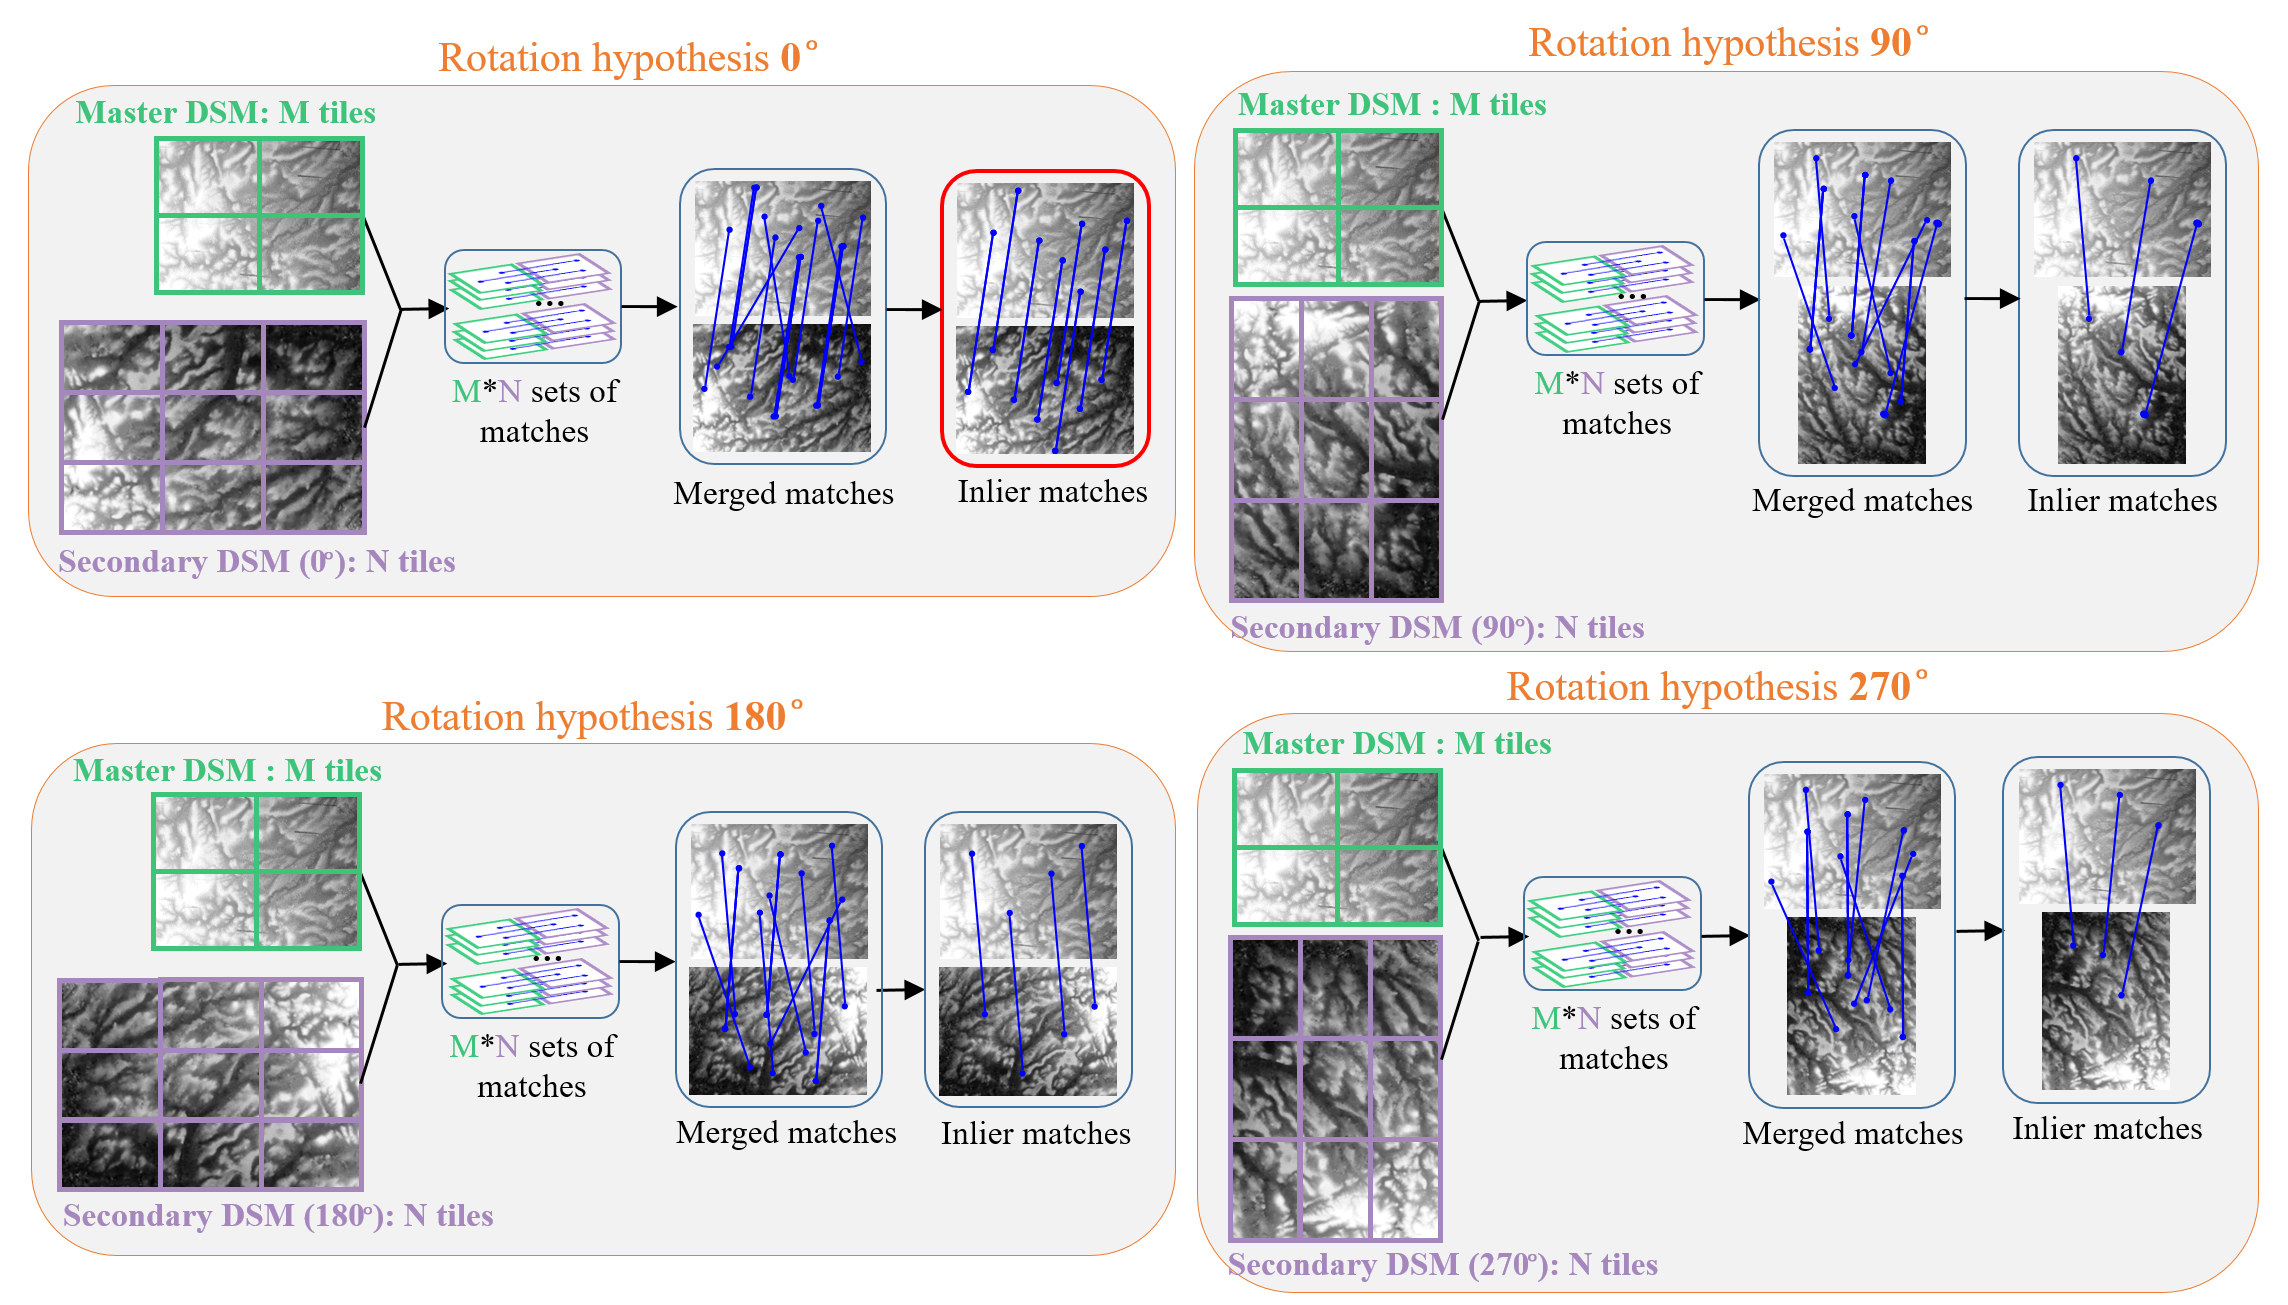
\includegraphics[width=0.8\columnwidth]{images/Chapitre3/dsm-RotHyp.png}
%        \caption{4 rotation hypotheses of matching DSMs.}
%        \label{Flow-process diagram}
%    \end{center}
%\end{figure*}

The DSM is converted to grayscale image as follows:\\
\begin{enumerate}
    \item Calculate the standard deviation of the DSM elevation;
    \item Pixels with elevations larger than double the standard deviation are considered outliers and therefore ignored;
    \item Transform the inlier pixels to the range of [0-255], resulting in grayscale image.
    \item Apply wallis filter on the grayscale image to get rid of uneven illumination, resulting in more informative image.
\end{enumerate}
\par
Matching DSMs/orthophotos has the following merits:
\begin{enumerate}
    \item Redundancy caused by the forward and side overlapping areas is removed;
    \item It enables a follow-up search for globally consistent inliers directly without the need to project matches onto ground;
    \item It decreases the combinatorial complexity caused by rotation ambiguity of P$\times$Q images;
    \item When matching DSMs, robust matches can be expected even under extreme scene changes, as 3D landscape generally provide stable information over time.
\end{enumerate}

DSMs/orthophotos are usually large images as they have larger extent than original images.
Learned matching methods often underperform on large images as they are either trained on small images in order to run real-time or with limited spatial resolution of CNN feature maps. We propose a \textit{one-to-many tiling scheme} to make up for the deficiency. 
\par
The \textit{one-to-many tiling scheme} is performed as follows (Figure~\ref{WorkflowOrtho}(a) and Figure~\ref{WorkflowDSM}(a)):\\
\begin{enumerate}
    \item Crop master and secondary images into M and N tiles of certain size (1280$\times$960 pixels in our experiments);
    \item Apply matching on M$\times$N tile pairs respectively;
    \item Merge the matches and perform RANSAC based on 2D similarity transformation to remove outliers.
\end{enumerate}                                   
In order to demonstrate if the \textit{one-to-many tiling scheme} helps, in Appendix ~\ref{chap:appendix2} we compared 2 sets of the results on matching multi-epoch orthophotos and DSMs: (1) $SuperGlue_{orig}$: SuperGlue without our \textit{one-to-many tiling scheme}; (2) $SuperGlue_{tiling}$: SuperGlue combined with our \textit{one-to-many tiling scheme}. As can be seen, $SuperGlue_{orig}$ failed while $SuperGlue_{tiling}$ recovered a large number of good matches.
\par
The \textit{one-to-many tiling scheme} can be combined with \textit{4 rotation hypotheses} when the matching method is both unsatisfactory on large images and not rotation invariant, as shown in Figure~\ref{WorkflowOrtho}(b) and Figure~\ref{WorkflowDSM}(b).
Both \textit{one-to-many tiling scheme} and \textit{4 rotation hypotheses} would not be applied when matching method that is satisfactory on large images and rotation invariant (e.g. SIFT) is adopted.
\par
The matching DSMs/orthophotos strategy works as follows:\\
\begin{enumerate}
    \item Transform DSMs to grayscale images if the DSMs are to be matched.
    \item Match DSMs/orthophotos (with or without \textit{one-to-many tiling scheme} and \textit{4 rotation hypotheses}, depending on whether the matching method is satisfactory on large images and rotation invariant), giving rise to one set of matches $M({\mathbf{K}^{e_1},\mathbf{K}^{e_2}})$ ($\mathbf{K}^{e_i}$ represents keypoints in DSM $D^{e_i}$ or orthophoto $Op^{e_i}$).
    %\item Run RANSAC on matches based on 2D similarity transformation model to remove outliers.
    \item Sample matches $M({\mathbf{K}^{e_1},\mathbf{K}^{e_2}})$ iteratively to compute the 2D similarity transformation RANSAC model:
\begin{equation}
\left [ \begin{array}{c}
{K}_x^{e_2}\\
{K}_y^{e_2}
\end{array}
\right ] =\lambda \cdot { \left[ \begin{array}{cc}
    cos\theta & sin\theta\\
    -sin\theta & cos\theta
    \end{array} 
    \right ]} \cdot {\left [ \begin{array}{c}
    {K}_x^{e_1}\\
    {K}_y^{e_1}
    \end{array}
    \right ]} + \left [ \begin{array}{c}
\Delta_x\\
\Delta_y
\end{array}
\right ]. \label{eq:2DSim}
\end{equation}

%   \begin{equation*}
%       {KG_i^{e_2}} = \lambda \cdot \mathbf{R} \cdot {KG_i^{e_1}} + \mathbf{T} , \quad i \in [1,3] \label{eq:3Dsim}
%   \end{equation*}
    where $\lambda$ is the scale factor, $\theta$ is the in-plane rotation angle and $\left [ \begin{array}{c}
    \Delta_x, \Delta_y
    \end{array}
    \right ]$ $^{^T}$ is the translation vector.
    %$\mathbf{T}$ is the translation vector and $\mathbf{R}$ is the rotation matrix.
    We set the number of RANSAC iterations to 1000, and consider matches within $T_r$ of its predicted position as inliers. In our experiment, {$T_r$ was set to 15 pixels.}
    \item Project the inlier matches onto ground to calculate 3D Helmert transformation parameters.
\end{enumerate}




%\subsubsection{SIFT}
%\subsubsection{SuperGlue}

\section{Experiments}
As described in the previous section, we provide 3 pipelines out of 2 strategies to perform rough co-registration:\\
\begin{enumerate}
	\item \textit{ImgPairs}: match image pairs;
	\item \textit{Ortho}: match orthophotos;
	\item \textit{DSM}: match DSMs.
\end{enumerate}
%\begin{enumerate}
%    \item Match image pairs: hereinafter referred to as \textit{ImgPairs};
%    \item Match orthophotos: hereinafter referred to as \textit{Ortho};
%    \item Match DSMs: hereinafter referred to as \textit{DSM}.
%\end{enumerate}
For each pipeline, we employ either SIFT or SuperGlue as the feature matching method, giving rise to 6 methods:\\
\begin{enumerate}
    \item $SIFT_{ImgPairs}$;
    \item $SuperGlue_{ImgPairs}$;
    \item $SIFT_{Ortho}$;
    \item $SuperGlue_{Ortho}$;
    \item $SIFT_{DSM}$;
    \item $SuperGlue_{DSM}$;
\end{enumerate}
In the following we introduce the implementation details, the datasets and the evaluation criteria, as well as comparison of the 6 methods.\\

\subsection{Implementation details}
\label{Implementationdetails}
%To improve efficiency, all input images are downsampled by a factor of 3 beforehand. To calculate the DSMs and orthophotos, we further downsample the images by a factor of 4, which amounts to a total downsampling factor of 12 with respect to the input images. For example, the images in Fr{\'e}jus 1970 are downsampled from [8766, 8763] to [730, 730]. As the goal of rough co-registration is to get robust rather than precise matches, a low resolution DSM/orthophoto is good enough and keeps the computational cost low. \\
To improve efficiency, all input images are downsampled by a factor of 3 beforehand. To calculate the DSMs and orthophotos, we further downsample the images by a factor of 8, which amounts to a total downsampling factor of 24 with respect to the input images. For example, the images in Fr{\'e}jus 1970 are downsampled from [8766, 8763] to [365, 365] for calculating DSMs and orthophotos. As the goal of rough co-registration is to get robust rather than precise matches, a low resolution DSM/orthophoto is good enough and keeps the computational cost low. \\
However, the downsampling factor of Fr{\'e}jus 2014 is set to be 12 instead of 24, as Fr{\'e}jus is mainly covered with buildings and the GSD of Fr{\'e}jus 2014 is too limited to tell details from DSM generated on images downsampled with factor 24.\\
%For each dataset, one epoch (generally the most recent epoch) would be chosen as the reference epoch, the remaining epochs would be treated as free epochs. The rough co-registration is applied on each free epoch and the reference epoch to obtain the co-registered image orientations in the frame of the reference epoch.
For each dataset, the rough co-registration is applied on each free epoch $E_f$ and the reference epoch $E_r$.
\par

%As inter-epoch images often look very different, when the original SIFT ~\cite{lowe2004distinctive} (i.e. $SIFT_{Default}$) is applied directly in our methods $SIFT_{ImgPairs}$, $SIFT_{Ortho}$ and $SIFT_{DSM}$, generally very few matches are recovered. So we replace it with a slightly different version of SIFT (i.e.  $SIFT_{Adapted}$) with the following modifications:\\
For the SIFT algorithm applied in methods $SIFT_{ImgPairs}$, $SIFT_{Ortho}$ and $SIFT_{DSM}$, we did a test to compare the performance of SIFT on multi-epoch dataset with different parameters. Two different sets of SIFT parameters are compared, which are referred to as $SIFT_{Default}$ and $SIFT_{Adapted}$:\\
\begin{enumerate}
	\item \textbf{$SIFT_{Default}$}: Extract SIFT keypoints on the original images, followed by mutual nearest neighbor matching combined with ratio test.% and FIGNN (REF).
	%\item \textbf{$SIFT_{Adapted}$}: Downsample the input images with a factor of 3 and extract SIFT keypoints, match them by mutual nearest neighbor without ratio test and FIGNN, followed by applying RANSAC based on 2D similarity transformation model to remove outliers.
	\item \textbf{$SIFT_{Adapted}$}: Downsample the input images with a factor of 3 and extract SIFT keypoints, match them by mutual nearest neighbor without ratio test, followed by applying RANSAC based on 2D similarity transformation model to remove outliers.
\end{enumerate}

%\begin{enumerate}
%	\item Downsample the images by a factor of 3 (i.e. a total downsampling factor of 9 with respect to the input images) to focus on the global outline of the scene for improving robustness;
%	\item Relax the matching restriction by skipping the ratio test to obtain more tentative matches followed by applying RANSAC based on 2D similarity transformation model to remove outliers.
%\end{enumerate}
Experiments comparing $SIFT_{Default}$ and $SIFT_{Adapted}$ on methods ${ImgPairs}$, ${Ortho}$ and ${DSM}$ are displayed in Appendix ~\ref{chap:appendix1}, in which $SIFT_{Adapted}$ recovered enough good matches while $SIFT_{Default}$ failed. It is reasonable as inter-epoch images often look very different, $SIFT_{Default}$ generally recover very few matches. By downsamping the images, we are able to focus on the global outline of the scene for improving robustness. 
%By relaxing the matching restriction of ratio test and FIGNN, right matches would be reserved while wrong matches would be removed in the subsequent RANSAC.\\
By relaxing the matching restriction of ratio test, right matches would be reserved while wrong matches would be removed in the subsequent RANSAC.\\

For $SuperGlue_{ImgPairs}$, $SuperGlue_{Ortho}$ and $SuperGlue_{DSM}$, the image/patch pairs entering SuperGlue are downsampled to 640$\times$480 pixels, as it is the default parameter provided by the author and guarantees the best performance. 
%For the tiling scheme in $SuperGlue_{Ortho}$ and $SuperGlue_{DSM}$, orthophotos/DSMs are split to tiles of the size 1280$\times$960 pixels.


\subsection{Datasets}
\label{Datasets}
%Frejus, Pezenas, Kobe\\
We tested our rough co-registration methods on 4 sets of datasets: Fr{\'e}jus, Pezenas, Kobe and Alberona. Details of the datasets are listed in Table~\ref{AerialData}, ~\ref{SatelliteData} and Figure~\ref{FrejusData},~\ref{PezenasData}, ~\ref{KobeData}.
\par
\paragraph{Fr{\'e}jus} It is a 15 $km^2$ rectangular area located in Fr{\'e}jus, a commune in southeastern France. The area is mainly covered with buildings along with scattered farmlands, except a half-moon-shaped bay located in south. We have four sets of aerial images acquired in 1954, 1966, 1970 and 2014. The epoch 2014 was acquired with the \ac{IGN}'s digital metric camera ~\cite{souchon2010ign}, its orientations are both in global reference frame and precise. Therefore it is treated as \ac{GT} during our processing (in other words, the epoch 2014 is chosen as the reference epoch). 
The area exhibits drastic scene changes in the 60-year period, as can be seen in Figure~\ref{FrejusEvolution}, where evolution of a subregion is displayed.\\
\paragraph{Pezenas} It is a 420 $km^2$ rectangular area located in Pezenas in the Occitanie region in southern France. The area is mainly covered with vegetation and several sparsely populated urban zones. We have at our disposal three sets of aerial images acquired in 1971, 1981 and 2015, and one set of satellite images acquired in 2014. Both the epoch 2014 and 2015 are treated as \ac{GT}. In this dataset we are interested in matching historical epochs (1971 and 1981) with aerial \ac{GT} and satellite \ac{GT} individually. The area exhibits changes in scene appearance in the 44-year period.\\
\paragraph{Kobe} It is a 90 $km^2$ area of irregular shape located in the north of Awaji Island, Japan. The well-known Kobe earthquake happened here in January 1995. We have two sets of aerial images: pre-event acquired in 1991 and post-event acquired in 1995. It is mainly covered with mountain area and narrow urban zones along the sea. There is no \ac{GT}, hence we chose the latter epoch (i.e. epoch 1995) as the reference epoch and measured 2 points on Google map to scale the result to metric units. In this dataset we are interested in localizing the earthquake fault.

\paragraph{Alberona} It is located in the province of Foggia and region of Apulia, in southeast Italy.

\begin{table}[htbp]
	\scriptsize %\footnotesize
	\centering
	\begin{tabular}{||c|c||c|c|c||c|c|c|c||c||}\hline
\multicolumn{2}{||c||}{ } &   F [pix] &   Wid [mm] &   Hei [mm] &   GSD [m] &   F. o. &   S. o. &   H  [m] &   Nb \\\hline
\multirow{4}{*}{Fr{\'e}jus} & E1954 & 23350 & 300 & 300 & \color{black}0.11 & 60\% & 20\% & 2500 & 19\\
& E1966 & 10230 & 180 & 180 & \color{black}0.17 & 60\% & 30\% & 1700 & 15\\
& E1970 & 10230 & 180 & 180 & 0.17 & 60\% & 30\% & 1700 & 19\\
& E2014 & \color{black}18281 & 99.28 & 72.42 & 0.35 & 60\% & 30\% & 6500 & 33\\\hline
\multirow{4}{*}{Pezenas} & E1971 & 7589 & 230 & 230 & 0.32 &    60\% &    20\% & 2400 & 57\\
& E1981 & 7607 & 230 & 230 & 0.59 & 60\% & 20\% & 4500 & 27\\
& \multirow{2}{*}{E2015} & 9967.5 & 47 & 35 & 0.46 & 60\% & 50\% & 4600 & 308\\
&  & 9204.5 & 50 & 36 & 0.5 & 60\% & 50\% & 4600 & 74\\\hline
\multirow{2}{*}{Kobe}& E1991& 7662 & 212 & 212 & 0.5 &    65\% &    35\% & 3800 & 15\\
& E1995& 7662 & 212 & 212 & 0.18 & 65\% & 65\% & 1400 & 83\\\hline

\multirow{2}{*}{Alberona}& E1954 & 7662 & 212 & 212 & 0.5 &    65\% &    35\% & 3800 & 15\\
& E2003 & 7662 & 212 & 212 & 0.18 & 65\% & 65\% & 1400 & 83\\\hline
	\end{tabular}
	\caption{Aerial dataset details of Fr{\'e}jus, Pezenas and Kobe. The 2015 acquisition of Pezenas is obtained with two sets of camera. E stands for epoch, F means focal length, Wid and Hei are the width and height of image, GSD is the ground sampling distance, F.o. and S.o. are forward and side overlap, H is the flying height, Nb is the number of images.}
	\label{AerialData}
\end{table}

\begin{table}[htbp]
    \scriptsize %\footnotesize
    \centering
    \begin{tabular}{||l|c|c|c|c||c|c|c|c||c|c||}\hline
        &\multicolumn{4}{c||}{Fr{\'e}jus}&\multicolumn{4}{c||}{Pezenas}&\multicolumn{2}{c||}{Kobe}\\\hline
                &E1954&E1966&E1970&E2014&E1971&E1981&\multicolumn{2}{c||}{E2015}&E1991&E1995\\\hline\hline
        F [pix]&23350&10230&10230&\color{black}18281&7589&7607&9967.5&9204.5&7662&7662\\
        %Size [mm]&\color{black}300,300&\color{black}180,180&\color{black}180,180&99.28,72.42&230230&230230&47,35&50,36&212212&212,212\\
        Wid [mm]&300&180&180&99.28&230&230&47&50&212&212\\
        Hei [mm]&300&180&180&72.42&230&230&35&36&212&212\\
        GSD [m]&\color{black}0.11&\color{black}0.17&0.17&0.35&0.32&0.59&0.46&0.5&0.5&0.18\\
        F. o.&60\%&60\%&60\%&60\%&   60\%&60\%&60\%&60\%&   65\%&65\%\\
        S. o.&20\%&30\%&30\%&30\%&   20\%&20\%&50\%&50\%&   35\%&65\%\\
        H  [m]&2500&1700&1700&6500&2400&4500&4600&4600&3800&1400\\
        Nb &19&15&19&33&57&27&308&74&15&83\\\hline
    \end{tabular}
    \caption{Aerial dataset details of Fr{\'e}jus, Pezenas and Kobe. The 2015 acquisition of Pezenas is obtained with two sets of camera. E stands for epoch, F means focal length, Wid and Hei are the width and height of image, GSD is the ground sampling distance, F.o. and S.o. are forward and side overlap, H is the flying height, Nb is the number of images.}
    \label{AerialData}
\end{table}

\begin{table}[htbp]
	\scriptsize %\footnotesize
	\centering
	\begin{tabular}{||l|c|c||}\hline
		& Master image & Secondary image\\\hline
		Constellation & Pleiades & Pleiades \\
		GSD [m] & 0.5 & 0.5\\
		Acquired date & 12/06/2014 & 12/06/2014 \\
		Number of lines & 38468 & 37710 \\
		Number of pixels per line & 34108 & 33392 \\
		Cloud cover & 3.9\% & 4.0\% \\
		Snow cover & 0\% & 0\% \\\hline
		%B/H?
	\end{tabular}
	\caption{Satellite dataset details of Pezenas. GSD means the ground sampling distance.}
	\label{SatelliteData}
\end{table}

\begin{figure*}[htbp]
    \begin{center}
        \subfigure[Fr{\'e}jus 1954 (19 images)]{
            \begin{minipage}[t]{0.4\linewidth}
                \centering
                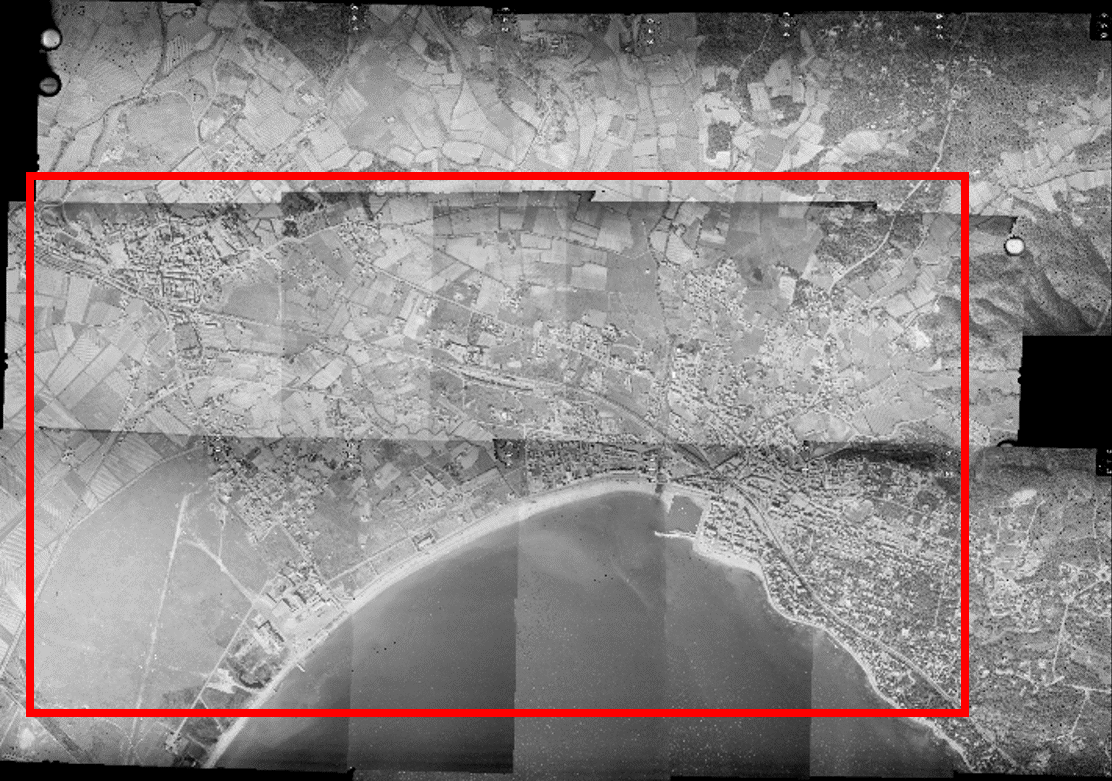
\includegraphics[width=5.65cm]{images/Chapitre3/Frejus1954.png}
            \end{minipage}%
        }
        \subfigure[Fr{\'e}jus 1966 (15 images)]{
            \begin{minipage}[t]{0.56\linewidth}
                \centering
                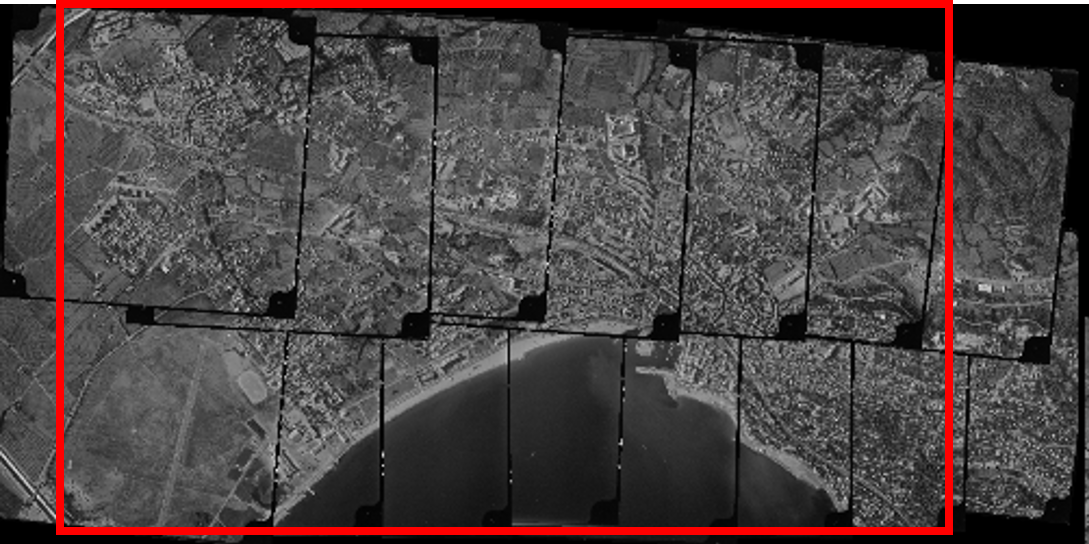
\includegraphics[width=7.6cm]{images/Chapitre3/Frejus1966.png}
            \end{minipage}%
        }
        \subfigure[Fr{\'e}jus 1970 (19 images)]{
    \begin{minipage}[t]{0.5\linewidth}
        \centering
        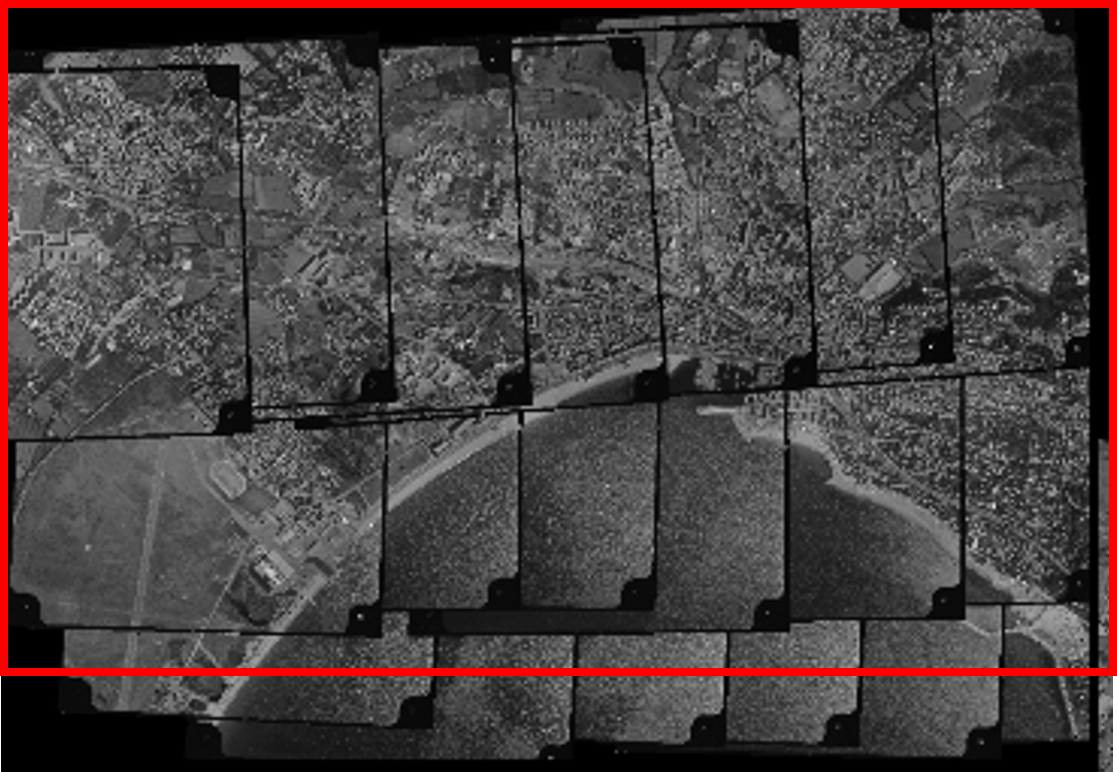
\includegraphics[width=6.1cm]{images/Chapitre3/Frejus1970.png}
    \end{minipage}%
}
\subfigure[Fr{\'e}jus 2014 (36 images)]{
    \begin{minipage}[t]{0.46\linewidth}
        \centering
        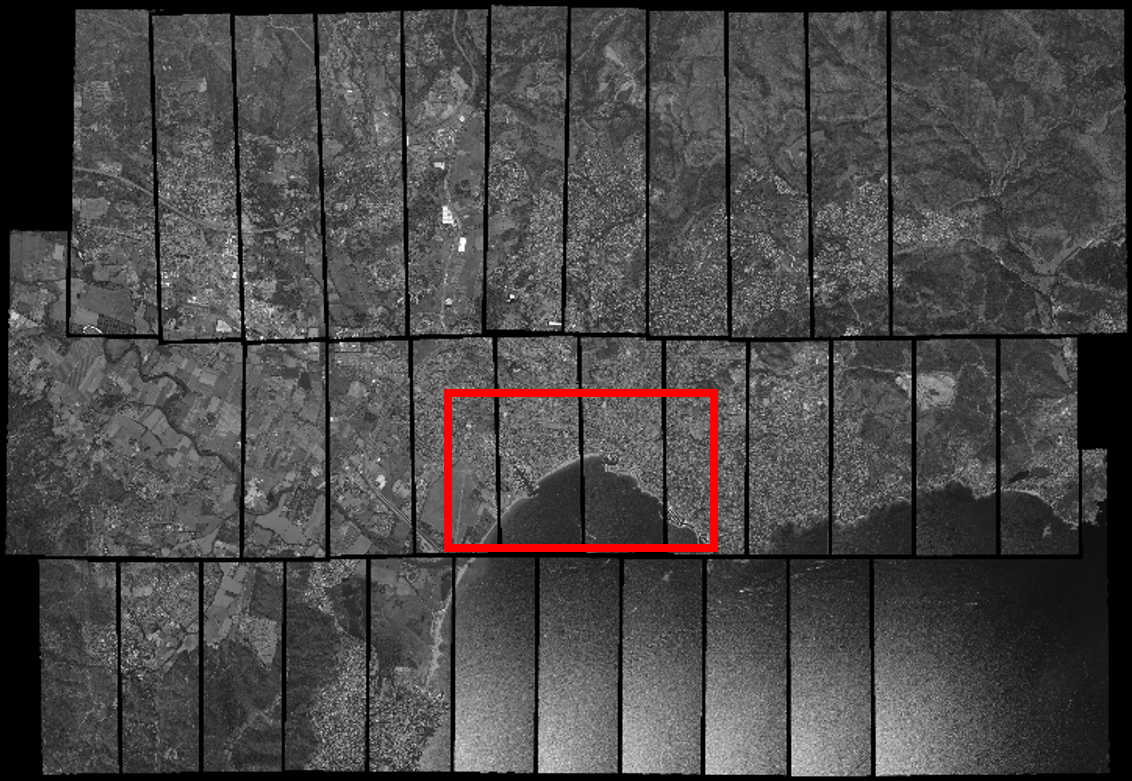
\includegraphics[width=6.25cm]{images/Chapitre3/Frejus2014.png}
    \end{minipage}%
}
        \caption{Images demonstration of different aerial epochs in Fr{\'e}jus, image number of each epoch is displayed in the parenthesis of each sub headline. The common zone between all the epochs is indicated by the red rectangles. Epoch 2014 is chosen as the reference epoch $E_r$ and the other epochs (i.e. epoch 1954, 1966 and 1970) are free epochs $E_f$ that should be co-registered to the frame of $E_r$. Graphic scale is demonstrated on $E_r$ in (d).}
        \label{FrejusData}
    \end{center}
\end{figure*} 


\begin{figure*}[htbp]
    \begin{center}
        \subfigure[Pezenas 1971 (57 images)]{
            \begin{minipage}[t]{0.48\linewidth}
                \centering
                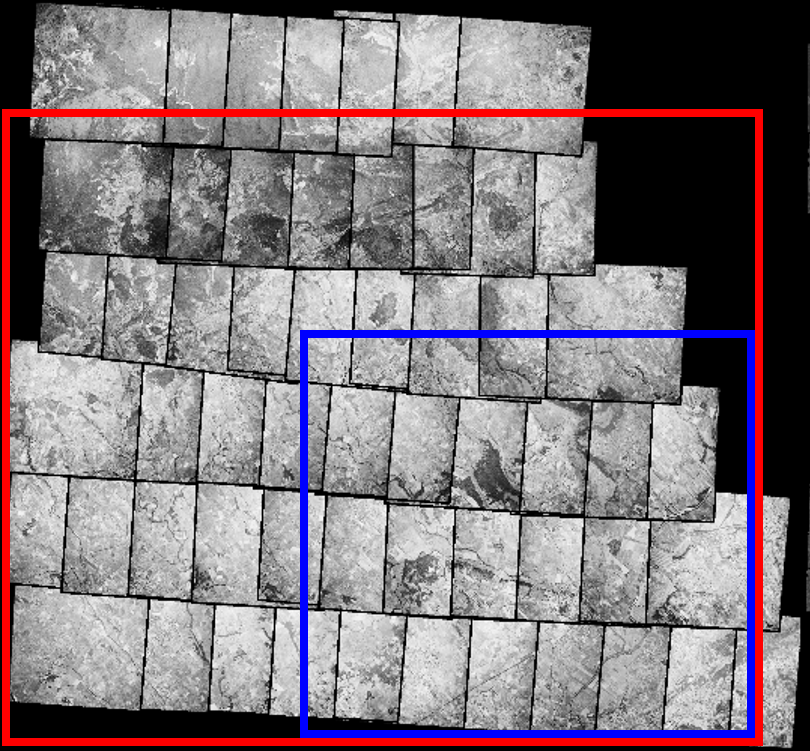
\includegraphics[width=6.45cm]{images/Chapitre3/Pezenas1971.png}
            \end{minipage}%
        }
        \subfigure[Pezenas 1981 (27 images)]{
            \begin{minipage}[t]{0.48\linewidth}
                \centering
                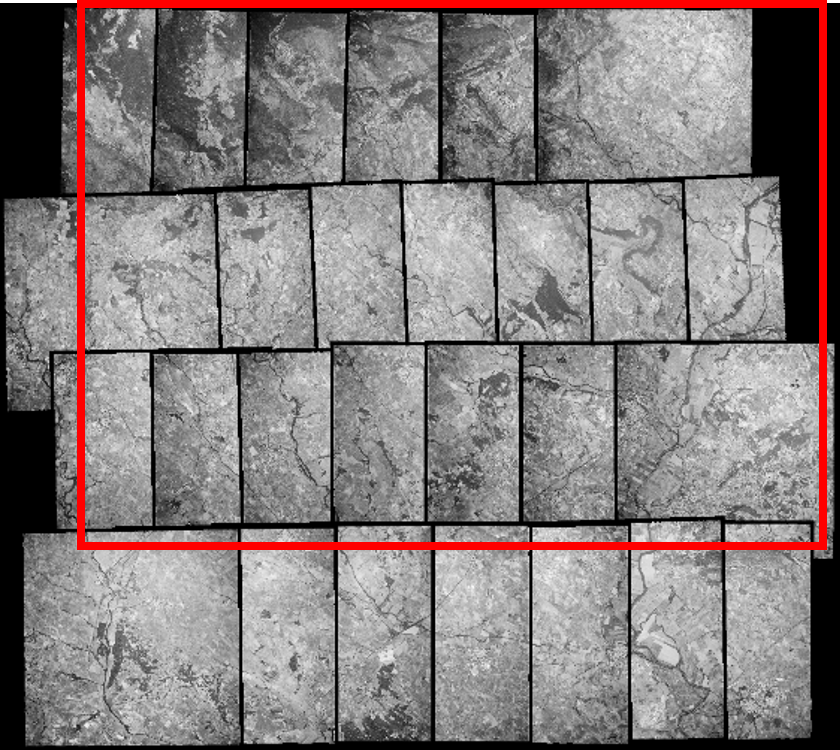
\includegraphics[width=6.68cm]{images/Chapitre3/Pezenas1981.png}
            \end{minipage}%
        }
            \subfigure[Pezenas 2014 (2 satellite images)]{
    	\begin{minipage}[t]{0.48\linewidth}
    		\centering
    		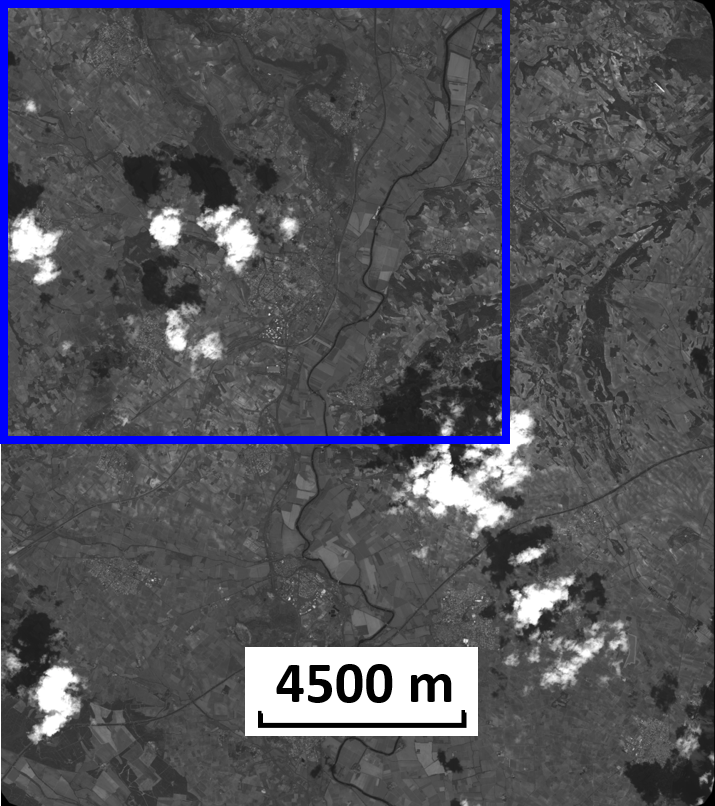
\includegraphics[width=6.6cm]{images/Chapitre3/Pezenas2014.png}
    	\end{minipage}%
    }
        \subfigure[Pezenas 2015 (382 images)]{
            \begin{minipage}[t]{0.48\linewidth}
                \centering
                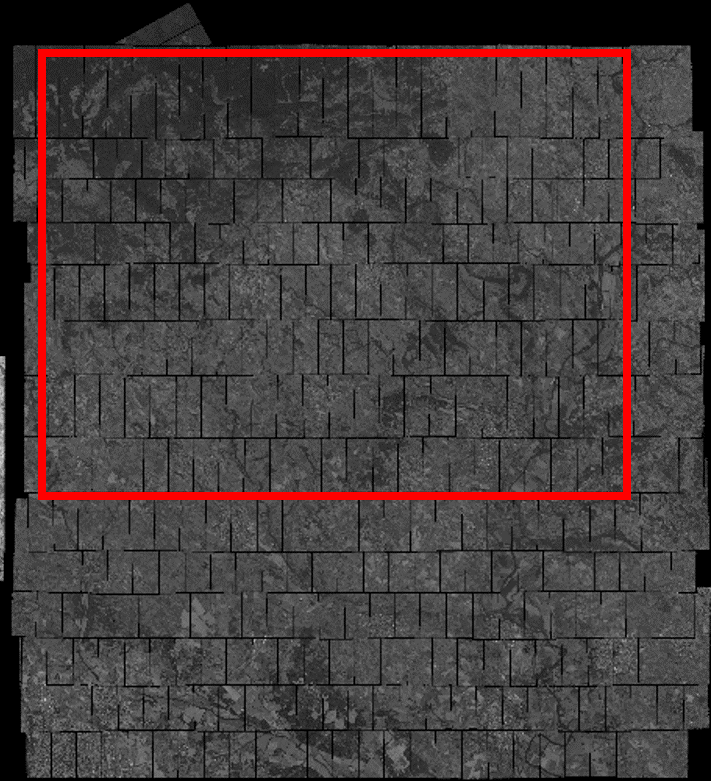
\includegraphics[width=6.78cm]{images/Chapitre3/Pezenas2015.png}
            \end{minipage}%
        }
        \caption{Images demonstration of different aerial epochs as well as satellite epoch in Pezenas, image number of each epoch is displayed in the parenthesis of each sub headline. There are 2 historical aerial epochs (1971 and 1981) and 2 \ac{GT} epochs (2014 the satellite epoch and 2015 the aerial epoch) in this dataset. The common zone between the historical epochs and the 2014 satellite epoch is indicated by the blue rectangles, while that between historical epochs and the 2015 aerial epoch is in red rectangles. Epoch 2014 and 2015 are chosen as the reference epoch $E_r$ and the other epochs (i.e. epoch 1971 and 1981) are free epochs $E_f$ that should be co-registered to the frame of $E_r$. Graphic scales are demonstrated on $E_r$ in (c) and (d).}
        \label{PezenasData}
    \end{center}
\end{figure*} 


\begin{figure*}[htbp]
    \begin{center}
        \subfigure[Kobe 1991 (15 images)]{
            \begin{minipage}[t]{1\linewidth}
                \centering
                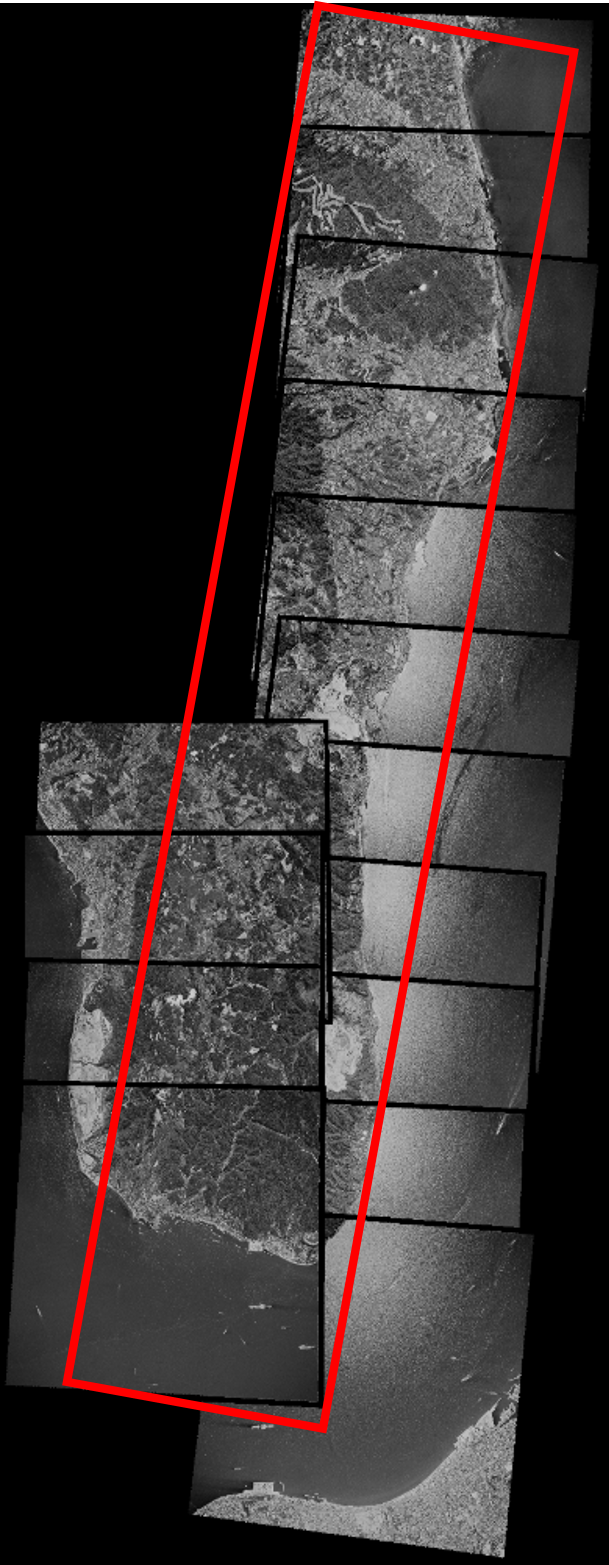
\includegraphics[height=13cm,angle=90]{images/Chapitre3/Kobe1991.png}
            \end{minipage}%
        }
        \subfigure[Kobe 1995 (83 images)]{
            \begin{minipage}[t]{1\linewidth}
                \centering
                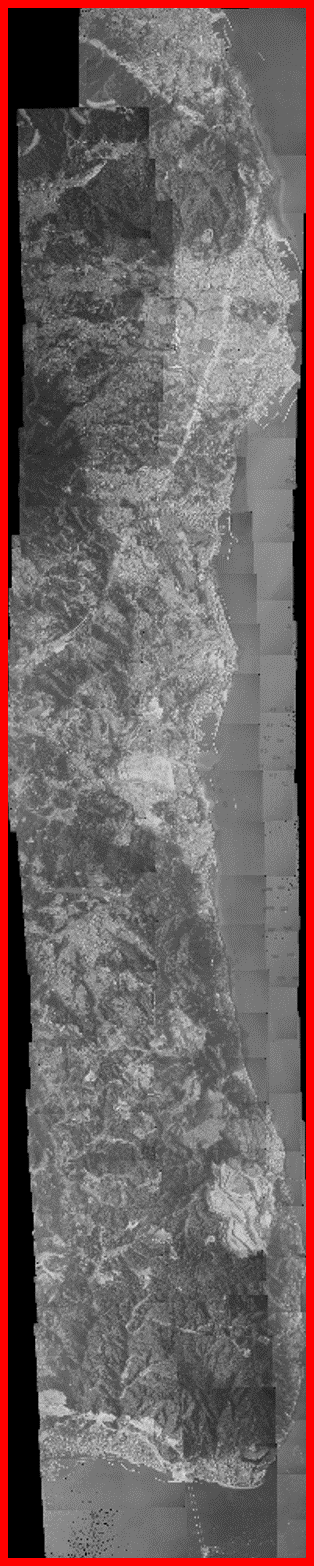
\includegraphics[height=13cm,angle=90]{images/Chapitre3/Kobe1995.png}
            \end{minipage}%
        }
        \caption{Images demonstration of different aerial epochs in Kobe, image number of each epoch is displayed in the parenthesis of each sub headline. The common zone between all the epochs is indicated by the red rectangles. Epoch 1995 is chosen as the reference epoch $E_r$ and the other epoch (i.e. epoch 1991) is free epoch $E_f$ that should be co-registered to the frame of $E_r$. Graphic scale is demonstrated on $E_r$ in (b).}
        \label{KobeData}
    \end{center}
\end{figure*} 


\begin{figure*}[htbp]
	\begin{center}
		\subfigure[Subregion of Fr{\'e}jus 1954]{
			\begin{minipage}[t]{1\linewidth}
				\centering
				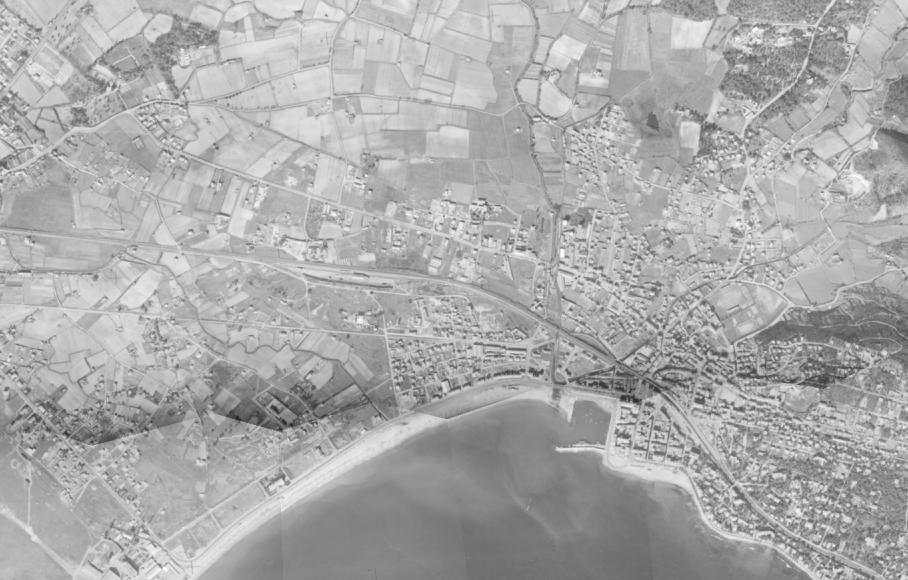
\includegraphics[width=13cm]{images/Chapitre3/Frejus1954Sub.png}
			\end{minipage}%
		}
		\subfigure[Subregion of Fr{\'e}jus 2014]{
			\begin{minipage}[t]{1\linewidth}
				\centering
				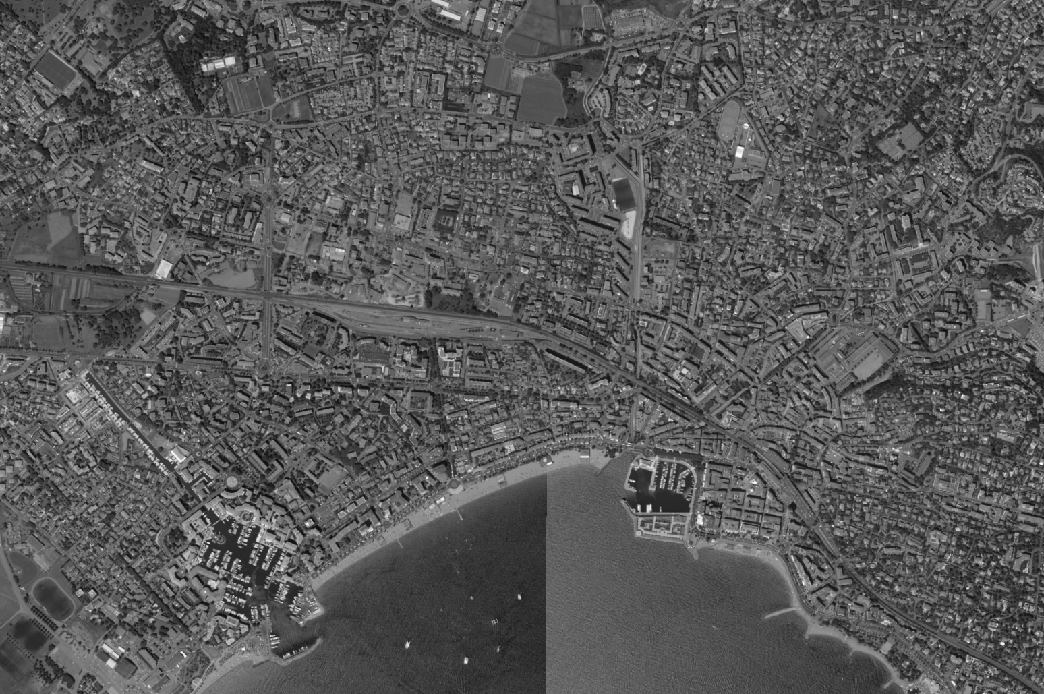
\includegraphics[width=13cm]{images/Chapitre3/Frejus2014Sub.png}
			\end{minipage}%
		}
		\caption{Evolution of a subregion in Fr{\'e}jus.}
		\label{FrejusEvolution}
	\end{center}
\end{figure*} 

%Show piled image of each epoch?
\subsection{Evaluation}
%%\subsubsection{Qualitative evaluation}
%%\subsubsection{Quantitative evaluation}
%%(1)Matches visualization\\
%%%inlier ratio (RANSAC and \ac{GT})\\
%%(2)Ground check points\\
%%(3)DoD\\
%For each dataset, we manually measured 3 GCPs well distributed in the block. The application of 3 GCPs is twofold:\\
%\begin{itemize}
%    \item Based on the GCPs, a 3D Helmert transformation model between each free epoch and the reference epoch is built to obtain the \ac{GT} co-registered orientations.
%    \item GCPs are also treated as ground check points to evaluate the co-registered orientations calculated by our methods.
%\end{itemize}
%%as check points to evaluate the roughly co-registered orientations resulted by 6 methods:\\
In order to evaluate the results qualitatively and quantitatively, the following criterias would be applied:\\
\begin{enumerate}
    \item \textbf{Matches visualization}. The number of (1) total matches (i.e. matches before RANSAC) as well as (2) RANSAC inliers (matches that survived RANSAC) would be displayed together in bar charts; in the meantime, the RANSAC inliers would be visualized and demonstrated, from which we can tell whether the methods succeeded or failed on each dataset.
%    \item Ground check points: the co-registered orientations calculated by our methods would be used to triangulate the ground check points and the coordinate differences \textcolor{red}{(explain the diff means the mean diff of x, y and z)} will be displayed. The better the epochs co-register, the smaller the difference is.
    \item \textbf{\ac{DoD}}. For the methods that succeeded, we use the resulted orientations in the same frame to calculate DSMs in order to generate \ac{DoD}. The visualization of \ac{DoD} as well as the statistical information would be displayed.
    %Ideally the DoD should only display the scene changes. If the dome effect appears, it indicates the systematic errors caused by poorly estimated camera parameters.   
\end{enumerate}

\subsection{Comparison}
%分三部分分别展示3组数据的结果
%3*2 methods:
%1张表表示6种方法的(1)和(2),1张大图放6种方法的DoD, inlier tie pt图(R3D, DSM, ortho各3张(无点图,SIFT点图,SpG点图))

\subsubsection{Matches visualization}
For each dataset, each free epoch $E_f$ is matched with reference epoch $E_r$ for rough co-registration with 6 methods (\ding{172} $SIFT_{ImgPairs}$, \ding{173} $SuperGlue_{ImgPairs}$, \ding{174} $SIFT_{Ortho}$, \ding{175} $SuperGlue_{Ortho}$, \ding{176} $SIFT_{DSM}$ and \ding{177} $SuperGlue_{DSM}$), the matches are visualized and displayed together for comparison. In Table~\ref{succeedorfail} we displayed whether the 6 methods succeeded or failed on each dataset.\\
\begin{enumerate}
	\item For Fr{\'e}jus, the reference epoch $E_r$ is 2014, the matches visualizations between free epochs $E_f$ (i.e. epoch 1954, 1966 and 1970) and $E_r$ are displayed in Figure~\ref{MatchVizFrejus1954DSM}, ~\ref{MatchVizFrejus1966DSM} and ~\ref{MatchVizFrejus1970DSM} individually. As can be seen, for all 3 free epochs:\\
	\begin{itemize}
		\item[-] $SIFT_{ImgPairs}$ and $SIFT_{Ortho}$ failed to recover correct matches. It is reasonable as extreme scene changes are present in Fr{\'e}jus, yet SIFT is not sufficiently invariant over time by its very nature.
		\item[-] $SIFT_{DSM}$ found several good matches after RANSAC, thanks to stable information on DSMs. However, the inlier ratio is dangerously low (around 1\%), which makes the RANSAC procedure unstable.
		\item[-] $SuperGlue_{ImgPairs}$, $SuperGlue_{Ortho}$ and $SuperGlue_{DSM}$ succeeded to find enough good matches, with the inlier ratios ranging from 3.3\% to 46.5\%. In general, the inlier ratios raise from $SuperGlue_{ImgPairs}$ to $SuperGlue_{Ortho}$ then to $SuperGlue_{DSM}$.
	\end{itemize}
	%$SIFT_{ImgPairs}$, $SuperGlue_{ImgPairs}$, $SIFT_{Ortho}$, $SuperGlue_{Ortho}$, $SIFT_{DSM}$ and $SuperGlue_{DSM}$
	\item For Pezenas, there are 2 reference epochs $E_r$:\\
	\begin{itemize}
	\item For aerial $E_r$ (i.e. epoch 2015), the matches visualizations between free epochs $E_f$ (i.e. epoch 1971 and 1981) and $E_r$ are displayed in Figure~\ref{MatchVizPezenas1971DSM} and ~\ref{MatchVizPezenas1981DSM}. As can be seen, for all 2 free epochs:\\
		\begin{itemize}
			\item[-] $SIFT_{ImgPairs}$, $SIFT_{Ortho}$ and $SIFT_{DSM}$ successfully recovered enough correct matches (with inlier ratios above 43\%, 1\% and 14\% individually). $SIFT_{Ortho}$ has obviously lower inlier ratio than $SIFT_{ImgPairs}$, because higher resolution is possessed by \textit{ImgPairs}, which improves the result for dataset with moderate scene changes like Pezenas.
			\item[-] $SuperGlue_{ImgPairs}$, $SuperGlue_{Ortho}$ and $SuperGlue_{DSM}$ recovered more total matches along with generally higher inlier ratio than SIFT. The inlier ratio of $SuperGlue_{Ortho}$ is above 76\%, significantly larger than $SIFT_{Ortho}$, which we attribute to 2 reasons: (1) SuperGlue is more invariant over time as it is trained on multi-epoch images and (2) our tiling scheme. 
		\end{itemize}
	\item For satellite $E_r$ (i.e. epoch 2014), the matches visualizations between free epochs $E_f$ (i.e. epoch 1971 and 1981) and $E_r$ are shown in Figure~\ref{MatchVizPezenas-Satellite1971DSM} and ~\ref{MatchVizPezenas-Satellite1981DSM}. As can be seen:\\
		\begin{itemize}
			\item[-] The results are inferior compared to the ones on aerial $E_r$, since satellite epoch not only has more limited zone overlapped with the free epochs, especially for epoch 1971, but also is covered with clouds.
			\item[-] $SIFT_{Ortho}$ failed on both free epochs, while $SIFT_{DSM}$ found enough good matches with inlier ratio around 4\%, as landscapes are more informative.
			\item[-] $SuperGlue_{Ortho}$ failed on epoch 1971 yet succeeded on epoch 1981, as larger common zone provides more clues in context to ensure the matching performance. $SuperGlue_{DSM}$ recovered more good matches with larger inlier ratio than $SIFT_{DSM}$ on both epochs.
		\end{itemize}
	\end{itemize}
	\item For Kobe, the reference epoch $E_r$ is 1995, the matches visualizations between free epoch $E_f$ (i.e. epoch 1991) and $E_r$ are displayed in Figure~\ref{MatchVizKobe1991DSM}.
		\begin{itemize}
		\item[-] $SIFT_{ImgPairs}$ and $SIFT_{Ortho}$ failed while $SIFT_{DSM}$ performs well.
		\item[-] $SuperGlue_{ImgPairs}$, $SuperGlue_{Ortho}$ and $SuperGlue_{DSM}$ successfully found good matches with inlier ratio over 32\% .
	\end{itemize}
\end{enumerate}

\begin{table}[htbp]
	\scriptsize %\footnotesize
	\centering
	\begin{tabular}{||l|c|c|c|c|c|c||}\hline
		&\multicolumn{2}{c|}{ImgPairs} &\multicolumn{2}{c|}{Ortho} &\multicolumn{2}{c|}{DSM}\\\hline
		& SIFT & SuperGlue & SIFT & SuperGlue & SIFT & SuperGlue \\\hline\hline
		%& $SIFT_{ImgPairs}$ & $SIFT_{Ortho}$ & $SIFT_{DSM}$ & $SuperGlue_{ImgPairs}$ & $SuperGlue_{Ortho}$ & $SuperGlue_{DSM}$\\\hline
%		$Frejus_{2014}^{1954}$ & Fail & Fail & \textbf{Succeed} & \textbf{Succeed} & \textbf{Succeed} & \textbf{Succeed} \\
%		$Frejus_{2014}^{1966}$ & Fail & Fail & \textbf{Succeed} & \textbf{Succeed} & \textbf{Succeed} & \textbf{Succeed} \\
%		$Frejus_{2014}^{1970}$ & Fail & Fail & \textbf{Succeed} & \textbf{Succeed} & \textbf{Succeed} & \textbf{Succeed} \\\hline
%		$Pezenas_{2015}^{1971}$ & \textbf{Succeed} & \textbf{Succeed} & \textbf{Succeed} & \textbf{Succeed} & \textbf{Succeed} & \textbf{Succeed} \\
%		$Pezenas_{2015}^{1981}$ & \textbf{Succeed} & \textbf{Succeed} & \textbf{Succeed} & \textbf{Succeed} & \textbf{Succeed} & \textbf{Succeed} \\\hline
%		$Pezenas_{2014(Satellite)}^{1971}$ & / & Fail & \textbf{Succeed} & / & Fail & \textbf{Succeed} \\
%		$Pezenas_{2014(Satellite)}^{1981}$ & / & Fail & \textbf{Succeed} & / & \textbf{Succeed} & \textbf{Succeed} \\\hline
%		$Frejus_{1995}^{1991}$ & Fail & Fail & \textbf{Succeed} & \textbf{Succeed} & \textbf{Succeed} & \textbf{Succeed} \\\hline
$Frejus_{2014}^{1954}$ &  Fail  &  \textbf{Succeed}  &  Fail  &  \textbf{Succeed}  &  \textbf{Succeed}  &  \textbf{Succeed} \\
$Frejus_{2014}^{1966}$ &  Fail  &  \textbf{Succeed}  &  Fail  &  \textbf{Succeed}  &  \textbf{Succeed}  &  \textbf{Succeed} \\
$Frejus_{2014}^{1970}$ &  Fail  &  \textbf{Succeed}  &  Fail  &  \textbf{Succeed}  &  \textbf{Succeed}  &  \textbf{Succeed} \\\hline
$Pezenas_{2015}^{1971}$ &  \textbf{Succeed}  &  \textbf{Succeed}  &  \textbf{Succeed}  &  \textbf{Succeed}  &  \textbf{Succeed}  &  \textbf{Succeed} \\
$Pezenas_{2015}^{1981}$ &  \textbf{Succeed}  &  \textbf{Succeed}  &  \textbf{Succeed}  &  \textbf{Succeed}  &  \textbf{Succeed}  &  \textbf{Succeed} \\\hline
$Pezenas_{2014(Satellite)}^{1971}$ & / & / &  Fail  &  Fail  &  \textbf{Succeed}  &  \textbf{Succeed} \\
$Pezenas_{2014(Satellite)}^{1981}$ & / & / &  Fail  &  \textbf{Succeed}  &  \textbf{Succeed}  &  \textbf{Succeed} \\\hline
$Frejus_{1995}^{1991}$ &  Fail  &  \textbf{Succeed}  &  Fail  &  \textbf{Succeed}  &  \textbf{Succeed}  &  \textbf{Succeed} \\\hline
	\end{tabular}
	\caption{Demonstration of 6 methods succeeding or failing on each dataset.}
	\label{succeedorfail}
\end{table}

In conclusion:\\
\begin{itemize}
	\item SuperGlue works better than SIFT for all the 3 pipelines (\textit{ImgPairs}, \textit{Ortho}, \textit{DSM}). 
	\item Pipeline \textit{DSM} gets better performance than \textit{ImgPairs} and \textit{Ortho}.
	\item Pipeline \textit{ImgPairs} often gets more numerous matches as they have higher resolution than \textit{Ortho} and \textit{DSM}, which leads to lower efficiency. However the performance is not necessarily better.
\end{itemize}

%Generally speaking, \textit{DSM} gets better performance than \textit{ImgPairs} and \textit{Ortho}. The result of \textit{ImgPairs} is not bad on 
%总结:变化不大时,ImgPairs效果最好
%ImgPairs效率最低

\begin{figure*}[htbp]
    \begin{center}
        \subfigure[Image pairs (19$\times$36 pairs)]{
            \begin{minipage}[t]{0.48\linewidth}
                \centering
                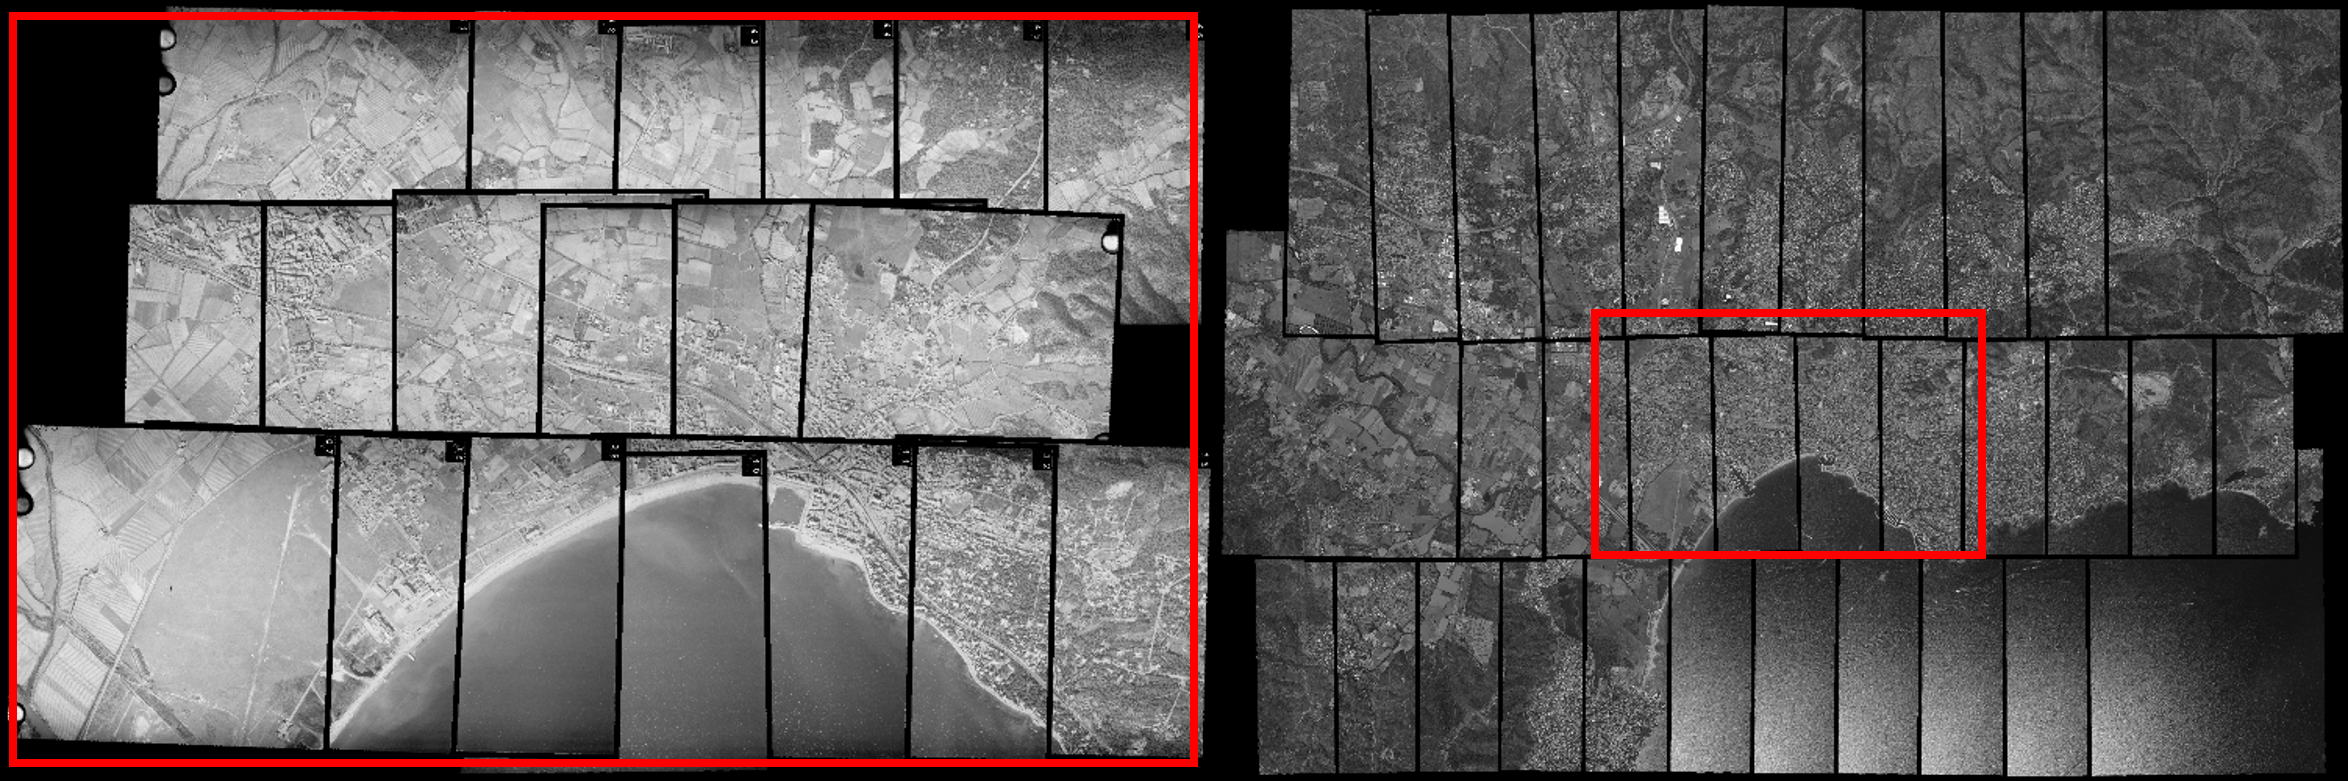
\includegraphics[width=6.8cm]{images/Chapitre3/Pseudo-Ortho-MEC-Malt_Tapas_1954_Ortho-MEC-Malt_2014.png}
            \end{minipage}%
        }
        \subfigure[Number of recovered matches(\textit{ImgPairs})]{
    \begin{minipage}[t]{0.48\linewidth}
        \centering
        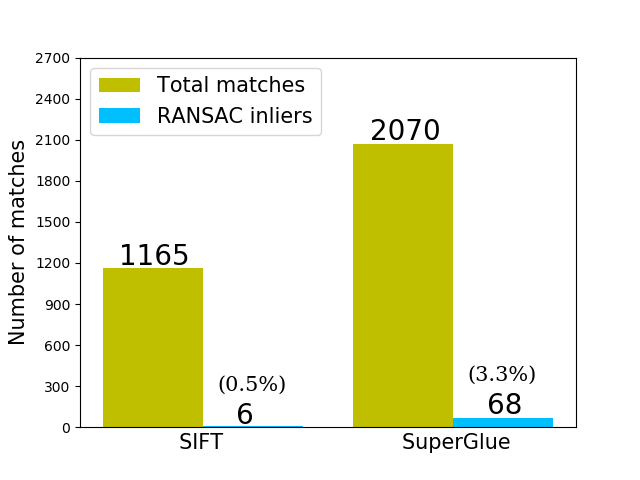
\includegraphics[width=3.5cm,trim=0 20 0 38,clip]{images/Chapitre3/PlotCurves_Pseudo-Ortho-MEC-Malt_Tapas_1954_Ortho-MEC-Malt_2014.png}
    \end{minipage}%
}
        \subfigure[$SIFT_{ImgPairs}^{RANSAC Inliers}$]{
            \begin{minipage}[t]{0.48\linewidth}
                \centering
                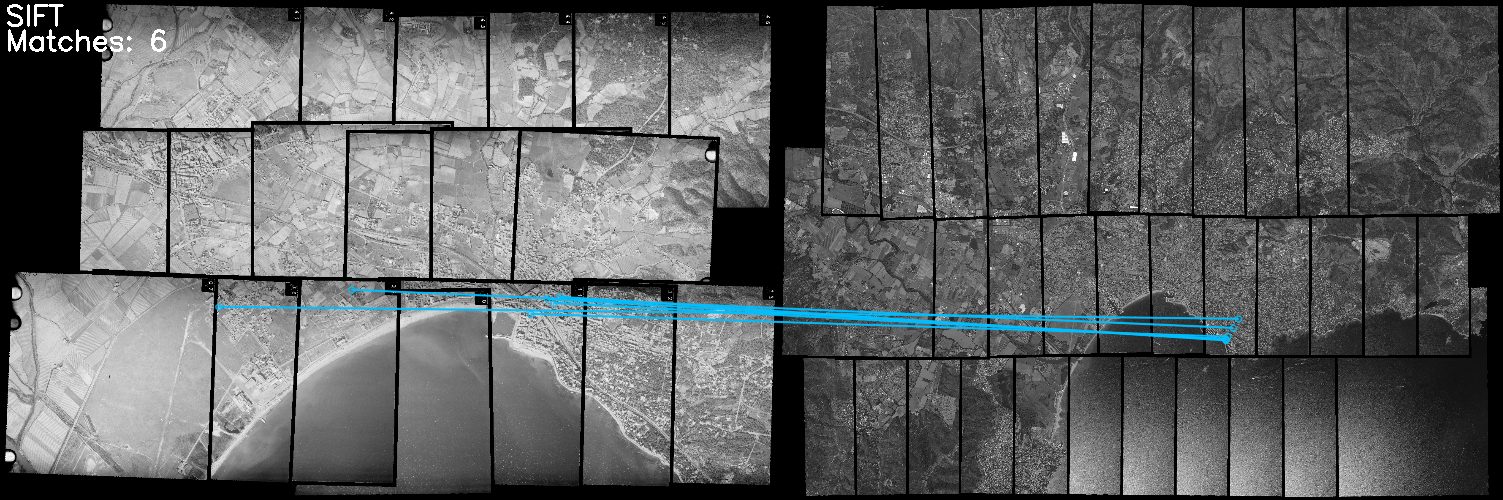
\includegraphics[width=6.8cm]{images/Chapitre3/Pseudo-Homol-SIFT2Step_1954-2014-Rough-2DRANSAC-GlobalR3D-PileImg_Ortho-MEC-Malt_Tapas_1954_Ortho-MEC-Malt_2014.png}
            \end{minipage}%
        }
        \subfigure[$SuperGlue_{ImgPairs}^{RANSAC Inliers}$]{
            \begin{minipage}[t]{0.48\linewidth}
                \centering
                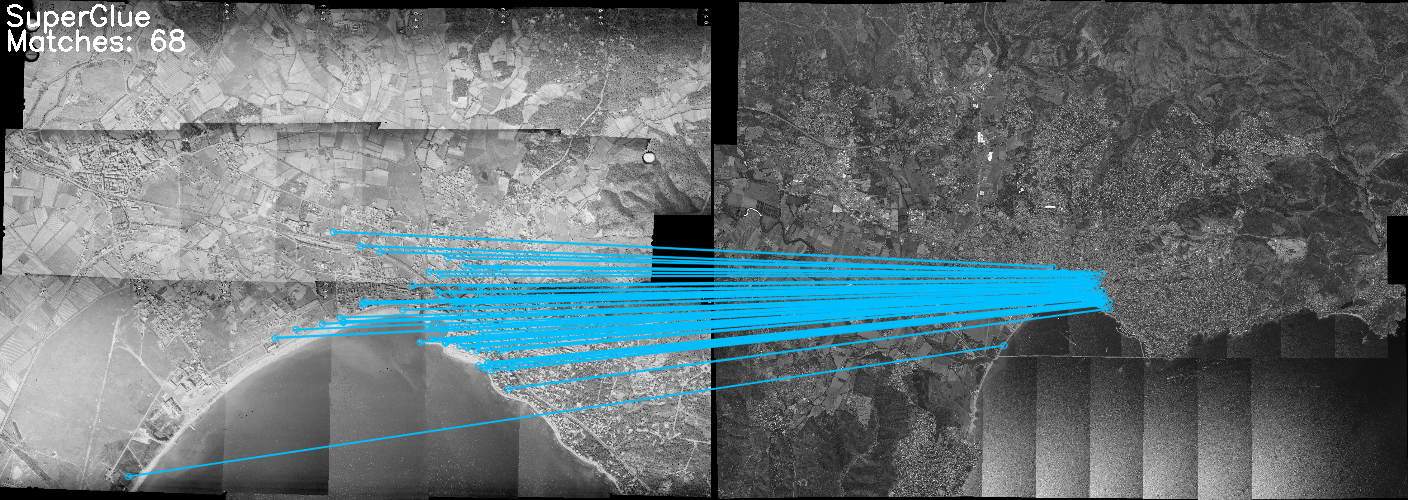
\includegraphics[width=6.8cm]{images/Chapitre3/Pseudo-Homol-SuperGlue_1954-2014-GlobalR3D-PileImg_Ortho-MEC-Malt_Tapas_1954_Ortho-MEC-Malt_2014.png}
            \end{minipage}%
        }
%        \caption{Result of matching image pairs (i.e. \textit{ImgPairs}) of Fr{\'e}jus 1954 and 2014. (a) Image pairs to be matched, with red rectangles indicating the common zone. (b) Numbers of total matches and RANSAC inliers of both SIFT and SuperGlue. (c) Visualization of RANSAC inliers based on SIFT. (d) Visualization of RANSAC inliers based on SuperGlue.}
%        \label{MatchVizFrejus1954ImgPairs}
%    \end{center}
%\end{figure*} 
%
%
%
%\begin{figure*}[htbp]
%    \begin{center}
        \subfigure[Orthophotos]{
    \begin{minipage}[t]{0.48\linewidth}
        \centering
        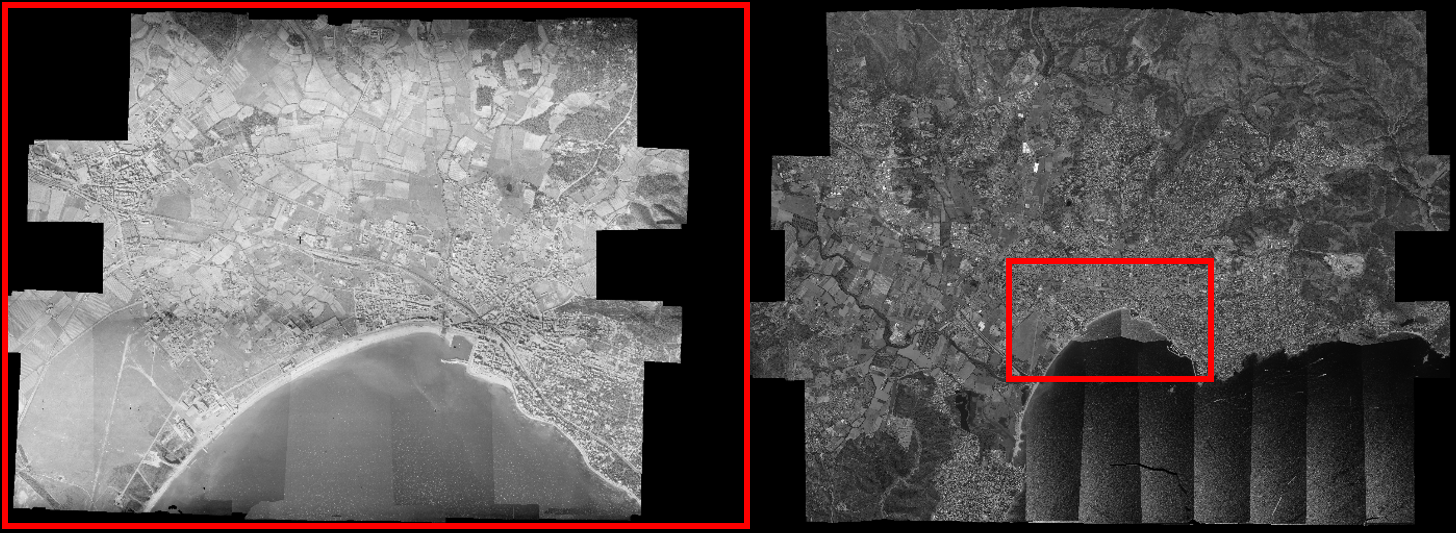
\includegraphics[width=6.8cm]{images/Chapitre3/Ortho-MEC-Malt_Tapas_1954_Ortho-MEC-Malt_2014.png}
    \end{minipage}%
}
\subfigure[Number of recovered matches(\textit{Ortho})]{
    \begin{minipage}[t]{0.48\linewidth}
        \centering
        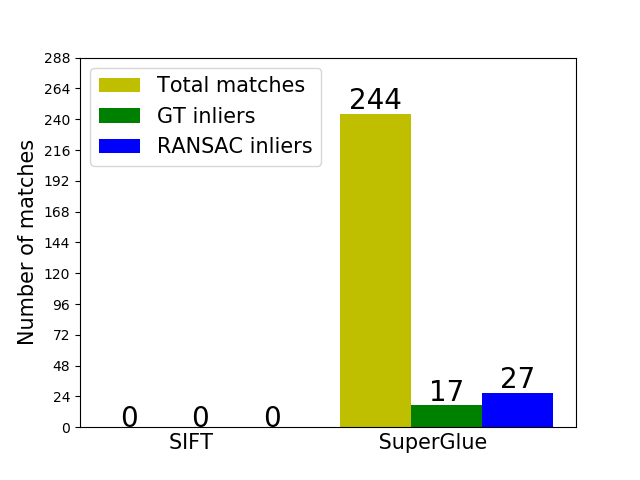
\includegraphics[width=3.5cm,trim=0 20 0 38,clip]{images/Chapitre3/PlotCurves_Ortho-MEC-Malt_Tapas_1954_Ortho-MEC-Malt_2014.png}
    \end{minipage}%
}
        \subfigure[$SIFT_{Ortho}^{RANSAC Inliers}$]{
            \begin{minipage}[t]{0.48\linewidth}
                \centering
                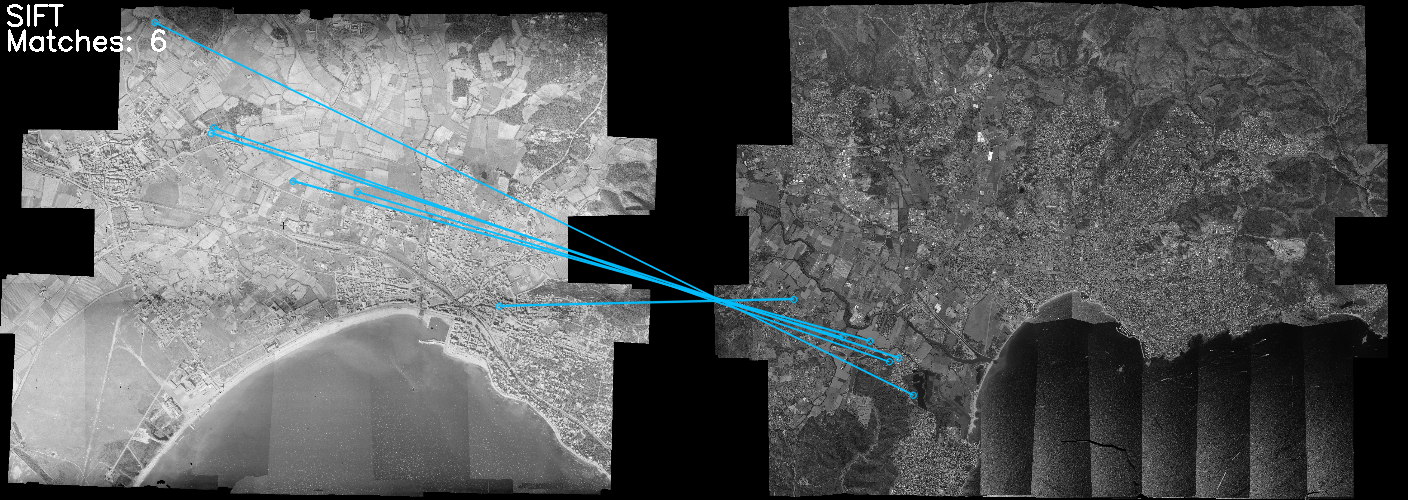
\includegraphics[width=6.8cm]{images/Chapitre3/Homol-SIFT2Step-Rough-2DRANSAC_Ortho-MEC-Malt_Tapas_1954_Ortho-MEC-Malt_2014.png}
            \end{minipage}%
        }
        \subfigure[$SuperGlue_{Ortho}^{RANSAC Inliers}$]{
            \begin{minipage}[t]{0.48\linewidth}
                \centering
                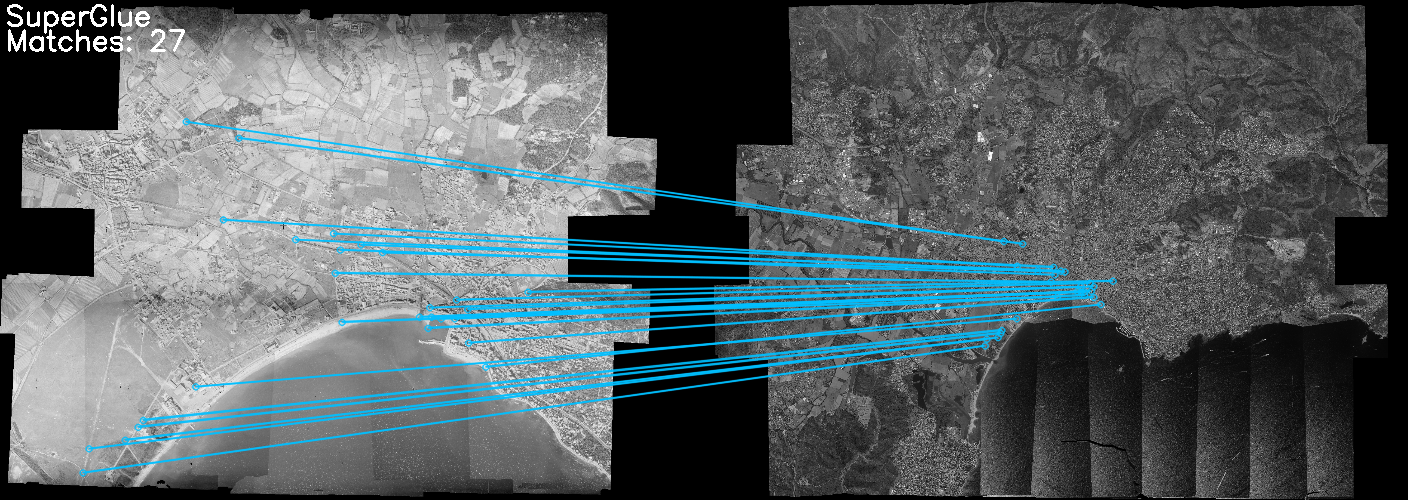
\includegraphics[width=6.8cm]{images/Chapitre3/Homol-SubPatch_R270-2DRANSAC_Ortho-MEC-Malt_Tapas_1954_Ortho-MEC-Malt_2014.png}
            \end{minipage}%
        }
%        \caption{Result of matching orthophotos (i.e. \textit{Ortho}) of Fr{\'e}jus 1954 and 2014. (a) Orthophotos to be matched, with red rectangles indicating the common zone. (b) Numbers of total matches and RANSAC inliers of both SIFT and SuperGlue. (c) Visualization of RANSAC inliers based on SIFT. (d) Visualization of RANSAC inliers based on SuperGlue.}
%        \label{MatchVizFrejus1954Ortho}
%    \end{center}
%\end{figure*} 
%
%\begin{figure*}[htbp]
%    \begin{center}
        \subfigure[DSMs]{
    \begin{minipage}[t]{0.48\linewidth}
        \centering
        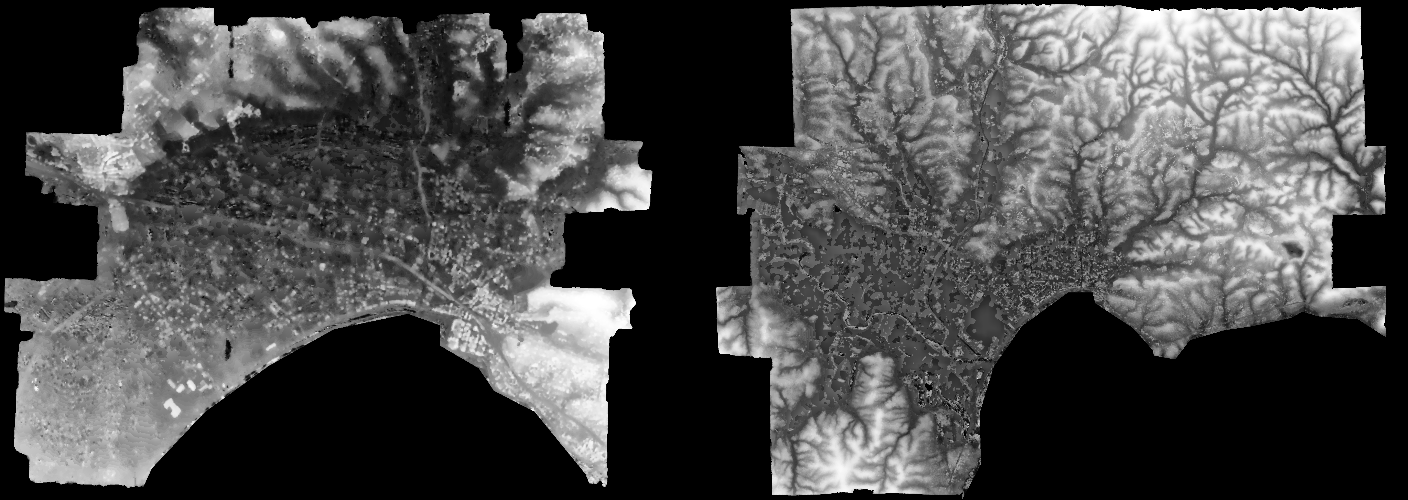
\includegraphics[width=6.8cm]{images/Chapitre3/MEC-Malt_Tapas_1954_MEC-Malt_2014.png}
    \end{minipage}%
}
\subfigure[Number of recovered matches(\textit{DSM})]{
    \begin{minipage}[t]{0.48\linewidth}
        \centering
        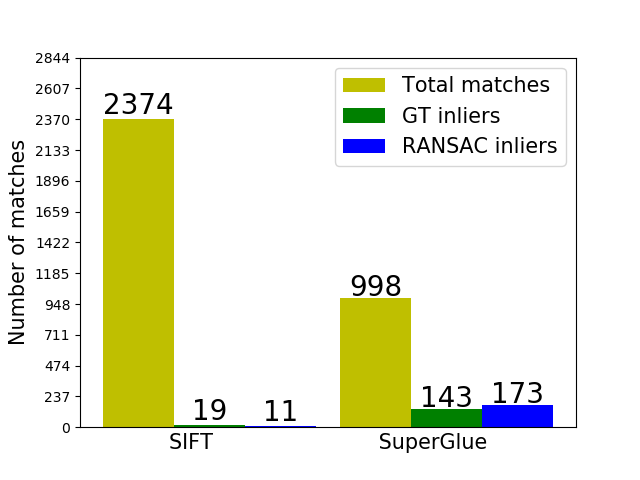
\includegraphics[width=3.5cm,trim=0 20 0 38,clip]{images/Chapitre3/PlotCurves_MEC-Malt_Tapas_1954_MEC-Malt_2014.png}
    \end{minipage}%
}
        \subfigure[$SIFT_{DSM}^{RANSAC Inliers}$]{
            \begin{minipage}[t]{0.48\linewidth}
                \centering
                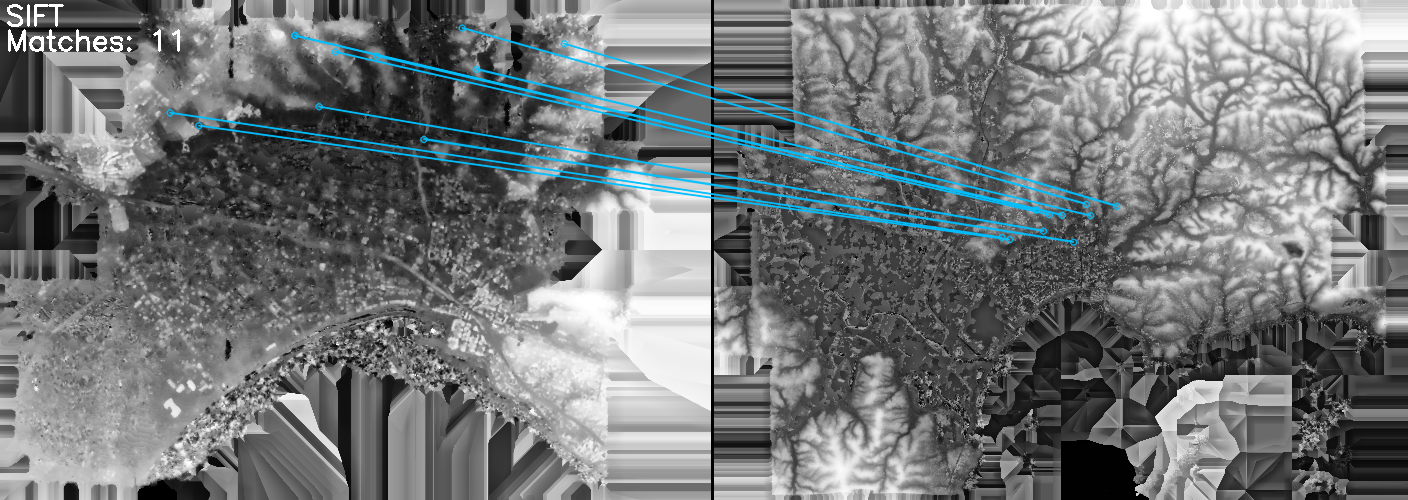
\includegraphics[width=6.8cm]{images/Chapitre3/Homol-SIFT2Step-Rough-2DRANSAC_MEC-Malt_Tapas_1954_MEC-Malt_2014.png}
            \end{minipage}%
        }
        \subfigure[$SuperGlue_{DSM}^{RANSAC Inliers}$]{
            \begin{minipage}[t]{0.48\linewidth}
                \centering
                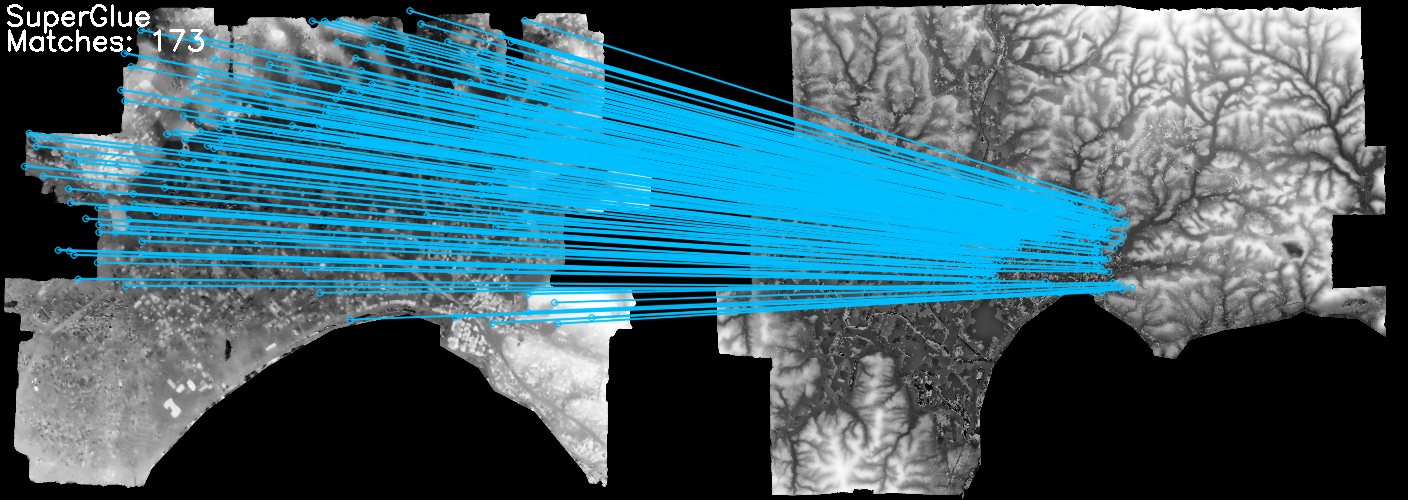
\includegraphics[width=6.8cm]{images/Chapitre3/Homol-SubPatch_R270-2DRANSAC_MEC-Malt_Tapas_1954_MEC-Malt_2014.png}
            \end{minipage}%
        }
        %\caption{Result of matching DSMs (i.e. \textit{DSM}) of Fr{\'e}jus 1954 and 2014. (a) DSMs to be matched, with red rectangles indicating the common zone. (b) Numbers of total matches and RANSAC inliers of both SIFT and SuperGlue. (c) Visualization of RANSAC inliers based on SIFT. (d) Visualization of RANSAC inliers based on SuperGlue.}
        \caption{{\scriptsize Result of \textit{ImgPairs} (a-d), \textit{Ortho} (e-h) and \textit{DSM} (i-l) on matching \textbf{Fr{\'e}jus 1954 and 2014}. (a, e, i) Image pairs/orthophotos/DSMs to be matched, with red rectangles indicating the common zone. (b, f, j) Numbers of total matches and RANSAC inliers of both SIFT and SuperGlue on methods \textit{ImgPairs}, \textit{Ortho} and \textit{DSM} individually. (c, g, k) Visualization of RANSAC inliers based on $SIFT_{ImgPairs}$, $SIFT_{Ortho}$ and $SIFT_{DSM}$. (d, h, l) Visualization of RANSAC inliers based on $SuperGlue_{ImgPairs}$, $SuperGlue_{Ortho}$ and $SuperGlue_{DSM}$.}}
        \label{MatchVizFrejus1954DSM}
    \end{center}
\end{figure*} 



\begin{figure*}[htbp]
    \begin{center}
        \subfigure[Image pairs (15$\times$36 pairs)]{
            \begin{minipage}[t]{0.48\linewidth}
                \centering
                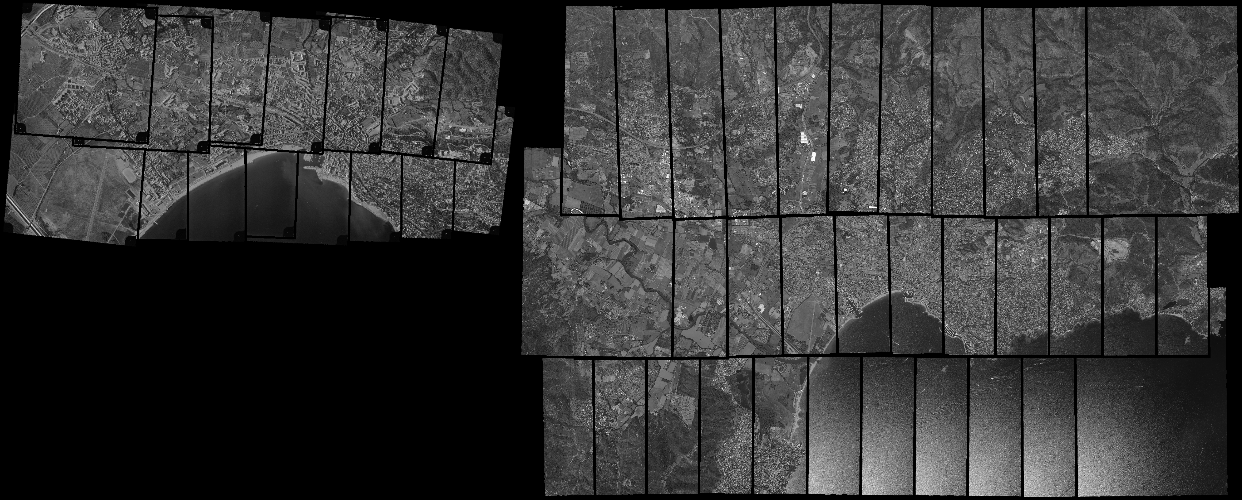
\includegraphics[width=6.1cm]{images/Chapitre3/Pseudo-Ortho-MEC-Malt_Tapas_1966_Ortho-MEC-Malt_2014.png}
            \end{minipage}%
        }
        \subfigure[Number of recovered matches(\textit{ImgPairs})]{
            \begin{minipage}[t]{0.48\linewidth}
                \centering
                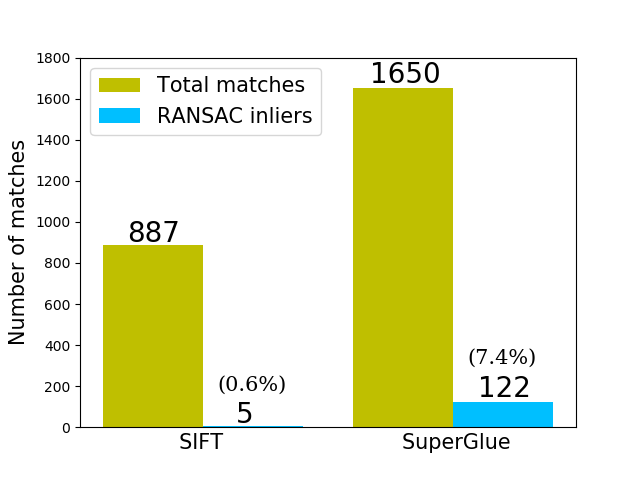
\includegraphics[width=3.5cm,trim=0 20 0 38,clip]{images/Chapitre3/PlotCurves_Pseudo-Ortho-MEC-Malt_Tapas_1966_Ortho-MEC-Malt_2014.png}
            \end{minipage}%
        }
        \subfigure[$SIFT_{ImgPairs}^{RANSAC Inliers}$]{
            \begin{minipage}[t]{0.48\linewidth}
                \centering
                \includegraphics[width=6cm]{images/Chapitre3/Pseudo-Homol-SIFT2Step_1966-2014-Rough-2DRANSAC-GlobalR3D-PileImg_Ortho-MEC-Malt_Tapas_1966_Ortho-MEC-Malt_2014.png}
            \end{minipage}%
        }
        \subfigure[$SuperGlue_{ImgPairs}^{RANSAC Inliers}$]{
            \begin{minipage}[t]{0.48\linewidth}
                \centering
                \includegraphics[width=6cm]{images/Chapitre3/Pseudo-Homol-SuperGlue_1966-2014-GlobalR3D-PileImg_Ortho-MEC-Malt_Tapas_1966_Ortho-MEC-Malt_2014.png}
            \end{minipage}%
        }
%        \caption{Result of matching image pairs (i.e. \textit{ImgPairs}) of Fr{\'e}jus 1966 and 2014. (a) Image pairs to be matched, with red rectangles indicating the common zone. (b) Numbers of total matches and RANSAC inliers of both SIFT and SuperGlue. (c) Visualization of RANSAC inliers based on SIFT. (d) Visualization of RANSAC inliers based on SuperGlue.}
%        \label{MatchVizFrejus1966ImgPairs}
%    \end{center}
%\end{figure*} 
%
%
%\begin{figure*}[htbp]
%    \begin{center}
        \subfigure[Orthophotos]{
            \begin{minipage}[t]{0.48\linewidth}
                \centering
                \includegraphics[width=6.1cm]{images/Chapitre3/Ortho-MEC-Malt_Tapas_1966_Ortho-MEC-Malt_2014.png}
            \end{minipage}%
        }
        \subfigure[Number of recovered matches(\textit{Ortho})]{
            \begin{minipage}[t]{0.48\linewidth}
                \centering
                \includegraphics[width=3.5cm,trim=0 20 0 38,clip]{images/Chapitre3/PlotCurves_Ortho-MEC-Malt_Tapas_1966_Ortho-MEC-Malt_2014.png}
            \end{minipage}%
        }
        \subfigure[$SIFT_{Ortho}^{RANSAC Inliers}$]{
            \begin{minipage}[t]{0.48\linewidth}
                \centering
                \includegraphics[width=6cm]{images/Chapitre3/Homol-SIFT2Step-Rough-2DRANSAC_Ortho-MEC-Malt_Tapas_1966_Ortho-MEC-Malt_2014.png}
            \end{minipage}%
        }
        \subfigure[$SuperGlue_{Ortho}^{RANSAC Inliers}$]{
            \begin{minipage}[t]{0.48\linewidth}
                \centering
                \includegraphics[width=6cm]{images/Chapitre3/Homol-SubPatch_R270-2DRANSAC_Ortho-MEC-Malt_Tapas_1966_Ortho-MEC-Malt_2014.png}
            \end{minipage}%
        }
%        \caption{Result of matching orthophotos (i.e. \textit{Ortho}) of Fr{\'e}jus 1966 and 2014. (a) Orthophotos to be matched, with red rectangles indicating the common zone. (b) Numbers of total matches and RANSAC inliers of both SIFT and SuperGlue. (c) Visualization of RANSAC inliers based on SIFT. (d) Visualization of RANSAC inliers based on SuperGlue.}
%        \label{MatchVizFrejus1966Ortho}
%    \end{center}
%\end{figure*} 
%
%\begin{figure*}[htbp]
%    \begin{center}
        \subfigure[DSMs]{
            \begin{minipage}[t]{0.48\linewidth}
                \centering
                \includegraphics[width=6.1cm]{images/Chapitre3/MEC-Malt_Tapas_1966_MEC-Malt_2014.png}
            \end{minipage}%
        }
        \subfigure[Number of recovered matches(\textit{DSM})]{
            \begin{minipage}[t]{0.48\linewidth}
                \centering
                \includegraphics[width=3.5cm,trim=0 20 0 38,clip]{images/Chapitre3/PlotCurves_MEC-Malt_Tapas_1966_MEC-Malt_2014.png}
            \end{minipage}%
        }
        \subfigure[$SIFT_{DSM}^{RANSAC Inliers}$]{
            \begin{minipage}[t]{0.48\linewidth}
                \centering
                \includegraphics[width=6cm]{images/Chapitre3/Homol-SIFT2Step-Rough-2DRANSAC_MEC-Malt_Tapas_1966_MEC-Malt_2014.png}
            \end{minipage}%
        }
        \subfigure[$SuperGlue_{DSM}^{RANSAC Inliers}$]{
            \begin{minipage}[t]{0.48\linewidth}
                \centering
                \includegraphics[width=6cm]{images/Chapitre3/Homol-SubPatch_R270-2DRANSAC_MEC-Malt_Tapas_1966_MEC-Malt_2014.png}
            \end{minipage}%
        }
        %\caption{Result of matching DSMs (i.e. \textit{DSM}) of Fr{\'e}jus 1966 and 2014. (a) DSMs to be matched, with red rectangles indicating the common zone. (b) Numbers of total matches and RANSAC inliers of both SIFT and SuperGlue. (c) Visualization of RANSAC inliers based on SIFT. (d) Visualization of RANSAC inliers based on SuperGlue.}
        %\caption{{\small Result of \textit{ImgPairs}, \textit{Ortho} and \textit{DSM} on Fr{\'e}jus 1966 and 2014. (a, e, i) Image pairs/orthophotos/DSMs to be matched, with red rectangles indicating the common zone. (b, f, j) Numbers of total matches and RANSAC inliers of both SIFT and SuperGlue on methods \textit{ImgPairs}, \textit{Ortho} and \textit{DSM} individually. (c, g, k) Visualization of RANSAC inliers based on $SIFT_{ImgPairs}$, $SIFT_{Ortho}$ and $SIFT_{DSM}$. (d, h, l) Visualization of RANSAC inliers based on $SuperGlue_{ImgPairs}$, $SuperGlue_{Ortho}$ and $SuperGlue_{DSM}$.}}
        \caption{{\scriptsize Result of \textit{ImgPairs} (a-d), \textit{Ortho} (e-h) and \textit{DSM} (i-l) on matching \textbf{Fr{\'e}jus 1966 and 2014}. (a, e, i) Image pairs/orthophotos/DSMs to be matched, with red rectangles indicating the common zone. (b, f, j) Numbers of total matches and RANSAC inliers of both SIFT and SuperGlue on methods \textit{ImgPairs}, \textit{Ortho} and \textit{DSM} individually. (c, g, k) Visualization of RANSAC inliers based on $SIFT_{ImgPairs}$, $SIFT_{Ortho}$ and $SIFT_{DSM}$. (d, h, l) Visualization of RANSAC inliers based on $SuperGlue_{ImgPairs}$, $SuperGlue_{Ortho}$ and $SuperGlue_{DSM}$.}}
        \label{MatchVizFrejus1966DSM}
    \end{center}
\end{figure*} 



\begin{figure*}[htbp]
    \begin{center}
        \subfigure[Image pairs (19$\times$36 pairs)]{
            \begin{minipage}[t]{0.48\linewidth}
                \centering
                \includegraphics[width=5.2cm]{images/Chapitre3/Pseudo-Ortho-MEC-Malt_Tapas_1970_Ortho-MEC-Malt_2014.png}
            \end{minipage}%
        }
        \subfigure[Number of recovered matches(\textit{ImgPairs})]{
            \begin{minipage}[t]{0.48\linewidth}
                \centering
                \includegraphics[width=3.5cm,trim=0 20 0 38,clip]{images/Chapitre3/PlotCurves_Pseudo-Ortho-MEC-Malt_Tapas_1970_Ortho-MEC-Malt_2014.png}
            \end{minipage}%
        }
        \subfigure[$SIFT_{ImgPairs}^{RANSAC Inliers}$]{
            \begin{minipage}[t]{0.48\linewidth}
                \centering
                \includegraphics[width=5.7cm]{images/Chapitre3/Pseudo-Homol-SIFT2Step_1970-2014-Rough-2DRANSAC-GlobalR3D-PileImg_Ortho-MEC-Malt_Tapas_1970_Ortho-MEC-Malt_2014.png}
            \end{minipage}%
        }
        \subfigure[$SuperGlue_{ImgPairs}^{RANSAC Inliers}$]{
            \begin{minipage}[t]{0.48\linewidth}
                \centering
                \includegraphics[width=5.7cm]{images/Chapitre3/Pseudo-Homol-SuperGlue_1970-2014-GlobalR3D-PileImg_Ortho-MEC-Malt_Tapas_1970_Ortho-MEC-Malt_2014.png}
            \end{minipage}%
        }
%        \caption{Result of matching image pairs (i.e. \textit{ImgPairs}) of Fr{\'e}jus 1970 and 2014. (a) Image pairs to be matched, with red rectangles indicating the common zone. (b) Numbers of total matches and RANSAC inliers of both SIFT and SuperGlue. (c) Visualization of RANSAC inliers based on SIFT. (d) Visualization of RANSAC inliers based on SuperGlue.}
%        \label{MatchVizFrejus1970ImgPairs}
%    \end{center}
%\end{figure*} 
%
%\begin{figure*}[htbp]
%    \begin{center}
        \subfigure[Orthophotos]{
            \begin{minipage}[t]{0.48\linewidth}
                \centering
                \includegraphics[width=5.2cm]{images/Chapitre3/Ortho-MEC-Malt_Tapas_1970_Ortho-MEC-Malt_2014.png}
            \end{minipage}%
        }
        \subfigure[Number of recovered matches(\textit{Ortho})]{
            \begin{minipage}[t]{0.48\linewidth}
                \centering
                \includegraphics[width=3.5cm,trim=0 20 0 38,clip]{images/Chapitre3/PlotCurves_Ortho-MEC-Malt_Tapas_1970_Ortho-MEC-Malt_2014.png}
            \end{minipage}%
        }
        \subfigure[$SIFT_{Ortho}^{RANSAC Inliers}$]{
            \begin{minipage}[t]{0.48\linewidth}
                \centering
                \includegraphics[width=5.7cm]{images/Chapitre3/Homol-SIFT2Step-Rough-2DRANSAC_Ortho-MEC-Malt_Tapas_1970_Ortho-MEC-Malt_2014.png}
            \end{minipage}%
        }
        \subfigure[$SuperGlue_{Ortho}^{RANSAC Inliers}$]{
            \begin{minipage}[t]{0.48\linewidth}
                \centering
                \includegraphics[width=5.7cm]{images/Chapitre3/Homol-SubPatch_R270-2DRANSAC_Ortho-MEC-Malt_Tapas_1970_Ortho-MEC-Malt_2014.png}
            \end{minipage}%
        }
%        \caption{Result of matching orthophotos (i.e. \textit{Ortho}) of Fr{\'e}jus 1970 and 2014. (a) Orthophotos to be matched, with red rectangles indicating the common zone. (b) Numbers of total matches and RANSAC inliers of both SIFT and SuperGlue. (c) Visualization of RANSAC inliers based on SIFT. (d) Visualization of RANSAC inliers based on SuperGlue.}
%        \label{MatchVizFrejus1970Ortho}
%    \end{center}
%\end{figure*} 
%
%\begin{figure*}[htbp]
%    \begin{center}
        \subfigure[DSMs]{
            \begin{minipage}[t]{0.48\linewidth}
                \centering
                \includegraphics[width=5.2cm]{images/Chapitre3/MEC-Malt_Tapas_1970_MEC-Malt_2014.png}
            \end{minipage}%
        }
        \subfigure[Number of recovered matches(\textit{DSM})]{
            \begin{minipage}[t]{0.48\linewidth}
                \centering
                \includegraphics[width=3.5cm,trim=0 20 0 38,clip]{images/Chapitre3/PlotCurves_MEC-Malt_Tapas_1970_MEC-Malt_2014.png}
            \end{minipage}%
        }
        \subfigure[$SIFT_{DSM}^{RANSAC Inliers}$]{
            \begin{minipage}[t]{0.48\linewidth}
                \centering
                \includegraphics[width=5.7cm]{images/Chapitre3/Homol-SIFT2Step-Rough-2DRANSAC_MEC-Malt_Tapas_1970_MEC-Malt_2014.png}
            \end{minipage}%
        }
        \subfigure[$SuperGlue_{DSM}^{RANSAC Inliers}$]{
            \begin{minipage}[t]{0.48\linewidth}
                \centering
                \includegraphics[width=5.7cm]{images/Chapitre3/Homol-SubPatch_R270-2DRANSAC_MEC-Malt_Tapas_1970_MEC-Malt_2014.png}
            \end{minipage}%
        }
        %\caption{Result of matching DSMs (i.e. \textit{DSM}) of Fr{\'e}jus 1970 and 2014. (a) DSMs to be matched, with red rectangles indicating the common zone. (b) Numbers of total matches and RANSAC inliers of both SIFT and SuperGlue. (c) Visualization of RANSAC inliers based on SIFT. (d) Visualization of RANSAC inliers based on SuperGlue.}
        %\caption{{\small Result of \textit{ImgPairs}, \textit{Ortho} and \textit{DSM} on Fr{\'e}jus 1970 and 2014. (a, e, i) image pairs/orthophotos/DSMs to be matched, with red rectangles indicating the common zone. (b, f, j) Numbers of total matches and RANSAC inliers of both SIFT and SuperGlue on methods \textit{ImgPairs}, \textit{Ortho} and \textit{DSM} individually. (c, g, k) Visualization of RANSAC inliers based on $SIFT_{ImgPairs}$, $SIFT_{Ortho}$ and $SIFT_{DSM}$. (d, h, l) Visualization of RANSAC inliers based on $SuperGlue_{ImgPairs}$, $SuperGlue_{Ortho}$ and $SuperGlue_{DSM}$.}}
        \caption{{\scriptsize Result of \textit{ImgPairs} (a-d), \textit{Ortho} (e-h) and \textit{DSM} (i-l) on matching \textbf{Fr{\'e}jus 1970 and 2014}. (a, e, i) Image pairs/orthophotos/DSMs to be matched, with red rectangles indicating the common zone. (b, f, j) Numbers of total matches and RANSAC inliers of both SIFT and SuperGlue on methods \textit{ImgPairs}, \textit{Ortho} and \textit{DSM} individually. (c, g, k) Visualization of RANSAC inliers based on $SIFT_{ImgPairs}$, $SIFT_{Ortho}$ and $SIFT_{DSM}$. (d, h, l) Visualization of RANSAC inliers based on $SuperGlue_{ImgPairs}$, $SuperGlue_{Ortho}$ and $SuperGlue_{DSM}$.}}
        \label{MatchVizFrejus1970DSM}
    \end{center}
\end{figure*} 


%%%%%%%%%%%%%%%%%%%%%%%%%%%%%%%%%%%%%%Pezenas Aerial
\begin{figure*}[htbp]
    \begin{center}
        \subfigure[Image pairs (57$\times$382 pairs)]{
            \begin{minipage}[t]{0.48\linewidth}
                \centering
                \includegraphics[width=5.1cm]{images/Chapitre3/Pseudo-Ortho-MEC-Malt_Tapas_1971_Ortho-MEC-Malt_2015.png}
            \end{minipage}%
        }
        \subfigure[Number of recovered matches(\textit{ImgPairs})]{
            \begin{minipage}[t]{0.48\linewidth}
                \centering
                \includegraphics[width=3.5cm,trim=0 20 0 38,clip]{images/Chapitre3/PlotCurves_Pseudo-Ortho-MEC-Malt_Tapas_1971_Ortho-MEC-Malt_2015.png}
            \end{minipage}%
        }
        \subfigure[$SIFT_{ImgPairs}^{RANSAC Inliers}$]{
            \begin{minipage}[t]{0.48\linewidth}
                \centering
                \includegraphics[width=5.2cm]{images/Chapitre3/Pseudo-Homol-SIFT2Step_1971-2015-Rough-2DRANSAC-GlobalR3D-PileImg_Ortho-MEC-Malt_Tapas_1971_Ortho-MEC-Malt_2015.png}
            \end{minipage}%
        }
        \subfigure[$SuperGlue_{ImgPairs}^{RANSAC Inliers}$]{
            \begin{minipage}[t]{0.48\linewidth}
                \centering
                \includegraphics[width=5.2cm]{images/Chapitre3/Pseudo-Homol-SuperGlue_1971-2015-GlobalR3D-PileImg_Ortho-MEC-Malt_Tapas_1971_Ortho-MEC-Malt_2015.png}
            \end{minipage}%
        }
%        \caption{Result of matching image pairs (i.e. \textit{ImgPairs}) of Pezenas 1971 and 2015. (a) Image pairs to be matched, with red rectangles indicating the common zone. (b) Numbers of total matches and RANSAC inliers of both SIFT and SuperGlue. (c) Visualization of RANSAC inliers based on SIFT. (d) Visualization of RANSAC inliers based on SuperGlue.}
%        \label{MatchVizPezenas1971ImgPairs}
%    \end{center}
%\end{figure*} 
%
%\begin{figure*}[htbp]
%    \begin{center}
        \subfigure[Orthophotos]{
            \begin{minipage}[t]{0.48\linewidth}
                \centering
                \includegraphics[width=5.1cm]{images/Chapitre3/Ortho-MEC-Malt_Tapas_1971_Ortho-MEC-Malt_2015.png}
            \end{minipage}%
        }
        \subfigure[Number of recovered matches(\textit{Ortho})]{
            \begin{minipage}[t]{0.48\linewidth}
                \centering
                \includegraphics[width=3.5cm,trim=0 20 0 38,clip]{images/Chapitre3/PlotCurves_Ortho-MEC-Malt_Tapas_1971_Ortho-MEC-Malt_2015.png}
            \end{minipage}%
        }
        \subfigure[$SIFT_{Ortho}^{RANSAC Inliers}$]{
            \begin{minipage}[t]{0.48\linewidth}
                \centering
                \includegraphics[width=5.2cm]{images/Chapitre3/Homol-SIFT2Step-Rough-2DRANSAC_Ortho-MEC-Malt_Tapas_1971_Ortho-MEC-Malt_2015.png}
            \end{minipage}%
        }
        \subfigure[$SuperGlue_{Ortho}^{RANSAC Inliers}$]{
            \begin{minipage}[t]{0.48\linewidth}
                \centering
                \includegraphics[width=5.2cm]{images/Chapitre3/Homol-SubPatch_R270-2DRANSAC_Ortho-MEC-Malt_Tapas_1971_Ortho-MEC-Malt_2015.png}
            \end{minipage}%
        }
%        \caption{Result of matching orthophotos (i.e. \textit{Ortho}) of Pezenas 1971 and 2015. (a) Orthophotos to be matched, with red rectangles indicating the common zone. (b) Numbers of total matches and RANSAC inliers of both SIFT and SuperGlue. (c) Visualization of RANSAC inliers based on SIFT. (d) Visualization of RANSAC inliers based on SuperGlue.}
%        \label{MatchVizPezenas1971Ortho}
%    \end{center}
%\end{figure*} 
%
%\begin{figure*}[htbp]
%    \begin{center}
        \subfigure[DSMs]{
            \begin{minipage}[t]{0.48\linewidth}
                \centering
                \includegraphics[width=5.1cm]{images/Chapitre3/MEC-Malt_Tapas_1971_MEC-Malt_2015.png}
            \end{minipage}%
        }
        \subfigure[Number of recovered matches(\textit{DSM})]{
            \begin{minipage}[t]{0.48\linewidth}
                \centering
                \includegraphics[width=3.5cm,trim=0 20 0 38,clip]{images/Chapitre3/PlotCurves_MEC-Malt_Tapas_1971_MEC-Malt_2015.png}
            \end{minipage}%
        }
        \subfigure[$SIFT_{DSM}^{RANSAC Inliers}$]{
            \begin{minipage}[t]{0.48\linewidth}
                \centering
                \includegraphics[width=5.2cm]{images/Chapitre3/Homol-SIFT2Step-Rough-2DRANSAC_MEC-Malt_Tapas_1971_MEC-Malt_2015.png}
            \end{minipage}%
        }
        \subfigure[$SuperGlue_{DSM}^{RANSAC Inliers}$]{
            \begin{minipage}[t]{0.48\linewidth}
                \centering
                \includegraphics[width=5.2cm]{images/Chapitre3/Homol-SubPatch_R270-2DRANSAC_MEC-Malt_Tapas_1971_MEC-Malt_2015.png}
            \end{minipage}%
        }
        %\caption{Result of matching DSMs (i.e. \textit{DSM}) of Pezenas 1971 and 2015. (a) DSMs to be matched, with red rectangles indicating the common zone. (b) Numbers of total matches and RANSAC inliers of both SIFT and SuperGlue. (c) Visualization of RANSAC inliers based on SIFT. (d) Visualization of RANSAC inliers based on SuperGlue.}
        %\caption{{\small Result of \textit{ImgPairs}, \textit{Ortho} and \textit{DSM} on Pezenas 1971 and 2015. (a, e, i) image pairs/orthophotos/DSMs to be matched, with red rectangles indicating the common zone. (b, f, j) Numbers of total matches and RANSAC inliers of both SIFT and SuperGlue on methods \textit{ImgPairs}, \textit{Ortho} and \textit{DSM} individually. (c, g, k) Visualization of RANSAC inliers based on $SIFT_{ImgPairs}$, $SIFT_{Ortho}$ and $SIFT_{DSM}$. (d, h, l) Visualization of RANSAC inliers based on $SuperGlue_{ImgPairs}$, $SuperGlue_{Ortho}$ and $SuperGlue_{DSM}$.}}
        \caption{{\scriptsize Result of \textit{ImgPairs} (a-d), \textit{Ortho} (e-h) and \textit{DSM} (i-l) on matching \textbf{Pezenas 1971 and 2015}. (a, e, i) Image pairs/orthophotos/DSMs to be matched, with red rectangles indicating the common zone. (b, f, j) Numbers of total matches and RANSAC inliers of both SIFT and SuperGlue on methods \textit{ImgPairs}, \textit{Ortho} and \textit{DSM} individually. (c, g, k) Visualization of RANSAC inliers based on $SIFT_{ImgPairs}$, $SIFT_{Ortho}$ and $SIFT_{DSM}$. (d, h, l) Visualization of RANSAC inliers based on $SuperGlue_{ImgPairs}$, $SuperGlue_{Ortho}$ and $SuperGlue_{DSM}$.}}        
        \label{MatchVizPezenas1971DSM}
    \end{center}
\end{figure*} 



\begin{figure*}[htbp]
    \begin{center}
        \subfigure[Image pairs (27$\times$382 pairs)]{
            \begin{minipage}[t]{0.48\linewidth}
                \centering
                \includegraphics[width=5.1cm]{images/Chapitre3/Pseudo-Ortho-MEC-Malt_Tapas_1981_Ortho-MEC-Malt_2015.png}
            \end{minipage}%
        }
        \subfigure[Number of recovered matches(\textit{ImgPairs})]{
            \begin{minipage}[t]{0.48\linewidth}
                \centering
                \includegraphics[width=3.5cm,trim=0 20 0 38,clip]{images/Chapitre3/PlotCurves_Pseudo-Ortho-MEC-Malt_Tapas_1981_Ortho-MEC-Malt_2015.png}
            \end{minipage}%
        }
        \subfigure[$SIFT_{ImgPairs}^{RANSAC Inliers}$]{
            \begin{minipage}[t]{0.48\linewidth}
                \centering
                \includegraphics[width=5.2cm]{images/Chapitre3/Pseudo-Homol-SIFT2Step_1981-2015-Rough-2DRANSAC-GlobalR3D-PileImg_Ortho-MEC-Malt_Tapas_1981_Ortho-MEC-Malt_2015.png}
            \end{minipage}%
        }
        \subfigure[$SuperGlue_{ImgPairs}^{RANSAC Inliers}$]{
            \begin{minipage}[t]{0.48\linewidth}
                \centering
                \includegraphics[width=5.2cm]{images/Chapitre3/Pseudo-Homol-SuperGlue_1981-2015-GlobalR3D-PileImg_Ortho-MEC-Malt_Tapas_1981_Ortho-MEC-Malt_2015.png}
            \end{minipage}%
        }
%        \caption{Result of matching image pairs (i.e. \textit{ImgPairs}) of Pezenas 1981 and 2015. (a) Image pairs to be matched, with red rectangles indicating the common zone. (b) Numbers of total matches and RANSAC inliers of both SIFT and SuperGlue. (c) Visualization of RANSAC inliers based on SIFT. (d) Visualization of RANSAC inliers based on SuperGlue.}
%        \label{MatchVizPezenas1981ImgPairs}
%    \end{center}
%\end{figure*} 
%
%\begin{figure*}[htbp]
%    \begin{center}
        \subfigure[Orthophotos]{
            \begin{minipage}[t]{0.48\linewidth}
                \centering
                \includegraphics[width=5.1cm]{images/Chapitre3/Ortho-MEC-Malt_Tapas_1981_Ortho-MEC-Malt_2015.png}
            \end{minipage}%
        }
        \subfigure[Number of recovered matches(\textit{Ortho})]{
            \begin{minipage}[t]{0.48\linewidth}
                \centering
                \includegraphics[width=3.5cm,trim=0 20 0 38,clip]{images/Chapitre3/PlotCurves_Ortho-MEC-Malt_Tapas_1981_Ortho-MEC-Malt_2015.png}
            \end{minipage}%
        }
        \subfigure[$SIFT_{Ortho}^{RANSAC Inliers}$]{
            \begin{minipage}[t]{0.48\linewidth}
                \centering
                \includegraphics[width=5.2cm]{images/Chapitre3/Homol-SIFT2Step-Rough-2DRANSAC_Ortho-MEC-Malt_Tapas_1981_Ortho-MEC-Malt_2015.png}
            \end{minipage}%
        }
        \subfigure[$SuperGlue_{Ortho}^{RANSAC Inliers}$]{
            \begin{minipage}[t]{0.48\linewidth}
                \centering
                \includegraphics[width=5.2cm]{images/Chapitre3/Homol-SubPatch_R90-2DRANSAC_Ortho-MEC-Malt_Tapas_1981_Ortho-MEC-Malt_2015.png}
            \end{minipage}%
        }
%        \caption{Result of matching orthophotos (i.e. \textit{Ortho}) of Pezenas 1981 and 2015. (a) Orthophotos to be matched, with red rectangles indicating the common zone. (b) Numbers of total matches and RANSAC inliers of both SIFT and SuperGlue. (c) Visualization of RANSAC inliers based on SIFT. (d) Visualization of RANSAC inliers based on SuperGlue.}
%        \label{MatchVizPezenas1981Ortho}
%    \end{center}
%\end{figure*} 
%
%\begin{figure*}[htbp]
%    \begin{center}
        \subfigure[DSMs]{
            \begin{minipage}[t]{0.48\linewidth}
                \centering
                \includegraphics[width=5.1cm]{images/Chapitre3/MEC-Malt_Tapas_1981_MEC-Malt_2015.png}
            \end{minipage}%
        }
        \subfigure[Number of recovered matches(\textit{DSM})]{
            \begin{minipage}[t]{0.48\linewidth}
                \centering
                \includegraphics[width=3.5cm,trim=0 20 0 38,clip]{images/Chapitre3/PlotCurves_MEC-Malt_Tapas_1981_MEC-Malt_2015.png}
            \end{minipage}%
        }
        \subfigure[$SIFT_{DSM}^{RANSAC Inliers}$]{
            \begin{minipage}[t]{0.48\linewidth}
                \centering
                \includegraphics[width=5.2cm]{images/Chapitre3/Homol-SIFT2Step-Rough-2DRANSAC_MEC-Malt_Tapas_1981_MEC-Malt_2015.png}
            \end{minipage}%
        }
        \subfigure[$SuperGlue_{DSM}^{RANSAC Inliers}$]{
            \begin{minipage}[t]{0.48\linewidth}
                \centering
                \includegraphics[width=5.2cm]{images/Chapitre3/Homol-SubPatch_R90-2DRANSAC_MEC-Malt_Tapas_1981_MEC-Malt_2015.png}
            \end{minipage}%
        }
        %\caption{Result of matching DSMs (i.e. \textit{DSM}) of Pezenas 1981 and 2015. (a) DSMs to be matched, with red rectangles indicating the common zone. (b) Numbers of total matches and RANSAC inliers of both SIFT and SuperGlue. (c) Visualization of RANSAC inliers based on SIFT. (d) Visualization of RANSAC inliers based on SuperGlue.}
        %\caption{{\small Result of \textit{ImgPairs}, \textit{Ortho} and \textit{DSM} on Pezenas 1981 and 2015. (a, e, i) image pairs/orthophotos/DSMs to be matched, with red rectangles indicating the common zone. (b, f, j) Numbers of total matches and RANSAC inliers of both SIFT and SuperGlue on methods \textit{ImgPairs}, \textit{Ortho} and \textit{DSM} individually. (c, g, k) Visualization of RANSAC inliers based on $SIFT_{ImgPairs}$, $SIFT_{Ortho}$ and $SIFT_{DSM}$. (d, h, l) Visualization of RANSAC inliers based on $SuperGlue_{ImgPairs}$, $SuperGlue_{Ortho}$ and $SuperGlue_{DSM}$.}}
        \caption{{\scriptsize Result of \textit{ImgPairs} (a-d), \textit{Ortho} (e-h) and \textit{DSM} (i-l) on matching \textbf{Pezenas 1981 and 2015}. (a, e, i) Image pairs/orthophotos/DSMs to be matched, with red rectangles indicating the common zone. (b, f, j) Numbers of total matches and RANSAC inliers of both SIFT and SuperGlue on methods \textit{ImgPairs}, \textit{Ortho} and \textit{DSM} individually. (c, g, k) Visualization of RANSAC inliers based on $SIFT_{ImgPairs}$, $SIFT_{Ortho}$ and $SIFT_{DSM}$. (d, h, l) Visualization of RANSAC inliers based on $SuperGlue_{ImgPairs}$, $SuperGlue_{Ortho}$ and $SuperGlue_{DSM}$.}}        
        \label{MatchVizPezenas1981DSM}
    \end{center}
\end{figure*} 



%%%%%%%%%%%%%%%%%%%%%%%%%%%%%%%%%%%%%%Pezenas Satellite
\begin{figure*}[htbp]
	\begin{center}
		\subfigure[Orthophotos]{
			\begin{minipage}[t]{0.48\linewidth}
				\centering
				\includegraphics[width=6.8cm]{images/Chapitre3/Ortho-MEC-Malt_Tapas_1971_Ortho-MEC-Malt_Satellite.png}
			\end{minipage}%
		}
		\subfigure[Number of recovered matches(\textit{Ortho})]{
			\begin{minipage}[t]{0.48\linewidth}
				\centering
				\includegraphics[width=4.9cm,trim=0 20 0 38,clip]{images/Chapitre3/PlotCurves_Ortho-MEC-Malt_Tapas_1971_Ortho-MEC-Malt_Satellite.png}
			\end{minipage}%
		}
		\subfigure[$SIFT_{Ortho}^{RANSAC Inliers}$]{
			\begin{minipage}[t]{0.48\linewidth}
				\centering
				\includegraphics[width=6.8cm]{images/Chapitre3/Homol-SIFT2Step-Rough-2DRANSAC_Ortho-MEC-Malt_Tapas_1971_Ortho-MEC-Malt_Satellite.png}
			\end{minipage}%
		}
		\subfigure[$SuperGlue_{Ortho}^{RANSAC Inliers}$]{
			\begin{minipage}[t]{0.48\linewidth}
				\centering
				\includegraphics[width=6.8cm]{images/Chapitre3/Homol-SubPatch_R270-2DRANSAC_Ortho-MEC-Malt_Tapas_1971_Ortho-MEC-Malt_Satellite.png}
			\end{minipage}%
		}
		%        \caption{Result of matching orthophotos (i.e. \textit{Ortho}) of Pezenas 1971 and Satellite. (a) Orthophotos to be matched, with red rectangles indicating the common zone. (b) Numbers of total matches and RANSAC inliers of both SIFT and SuperGlue. (c) Visualization of RANSAC inliers based on SIFT. (d) Visualization of RANSAC inliers based on SuperGlue.}
		%        \label{MatchVizPezenas-Satellite1971Ortho}
		%    \end{center}
		%\end{figure*} 
		%
		%\begin{figure*}[htbp]
		%    \begin{center}
		\subfigure[DSMs]{
			\begin{minipage}[t]{0.48\linewidth}
				\centering
				\includegraphics[width=6.8cm]{images/Chapitre3/MEC-Malt_Tapas_1971_MEC-Malt_Satellite.png}
			\end{minipage}%
		}
		\subfigure[Number of recovered matches(\textit{DSM})]{
			\begin{minipage}[t]{0.48\linewidth}
				\centering
				\includegraphics[width=4.9cm,trim=0 20 0 38,clip]{images/Chapitre3/PlotCurves_MEC-Malt_Tapas_1971_MEC-Malt_Satellite.png}
			\end{minipage}%
		}
		\subfigure[$SIFT_{DSM}^{RANSAC Inliers}$]{
			\begin{minipage}[t]{0.48\linewidth}
				\centering
				\includegraphics[width=6.8cm]{images/Chapitre3/Homol-SIFT2Step-Rough-2DRANSAC_MEC-Malt_Tapas_1971_MEC-Malt_Satellite.png}
			\end{minipage}%
		}
		\subfigure[$SuperGlue_{DSM}^{RANSAC Inliers}$]{
			\begin{minipage}[t]{0.48\linewidth}
				\centering
				\includegraphics[width=6.8cm]{images/Chapitre3/Homol-SubPatch_R270-2DRANSAC_MEC-Malt_Tapas_1971_MEC-Malt_Satellite.png}
			\end{minipage}%
		}
		%\caption{Result of matching DSMs (i.e. \textit{DSM}) of Pezenas 1971 and Satellite. (a) DSMs to be matched, with red rectangles indicating the common zone. (b) Numbers of total matches and RANSAC inliers of both SIFT and SuperGlue. (c) Visualization of RANSAC inliers based on SIFT. (d) Visualization of RANSAC inliers based on SuperGlue.}
		%\caption{{\small Result of \textit{ImgPairs}, \textit{Ortho} and \textit{DSM} on Pezenas 1971 and Satellite. (a, e, i) image pairs/orthophotos/DSMs to be matched, with red rectangles indicating the common zone. (b, f, j) Numbers of total matches and RANSAC inliers of both SIFT and SuperGlue on methods \textit{ImgPairs}, \textit{Ortho} and \textit{DSM} individually. (c, g, k) Visualization of RANSAC inliers based on $SIFT_{ImgPairs}$, $SIFT_{Ortho}$ and $SIFT_{DSM}$. (d, h, l) Visualization of RANSAC inliers based on $SuperGlue_{ImgPairs}$, $SuperGlue_{Ortho}$ and $SuperGlue_{DSM}$.}}
		\caption{{\scriptsize Result of \textit{ImgPairs} (a-d), \textit{Ortho} (e-h) and \textit{DSM} (i-l) on matching \textbf{Pezenas 1971 and 2014 (Satellite)}. (a, e, i) Image pairs/orthophotos/DSMs to be matched, with red rectangles indicating the common zone. (b, f, j) Numbers of total matches and RANSAC inliers of both SIFT and SuperGlue on methods \textit{ImgPairs}, \textit{Ortho} and \textit{DSM} individually. (c, g, k) Visualization of RANSAC inliers based on $SIFT_{ImgPairs}$, $SIFT_{Ortho}$ and $SIFT_{DSM}$. (d, h, l) Visualization of RANSAC inliers based on $SuperGlue_{ImgPairs}$, $SuperGlue_{Ortho}$ and $SuperGlue_{DSM}$.}}        
		\label{MatchVizPezenas-Satellite1971DSM}
	\end{center}
\end{figure*} 



\begin{figure*}[htbp]
	\begin{center}
		\subfigure[Orthophotos]{
			\begin{minipage}[t]{0.48\linewidth}
				\centering
				\includegraphics[width=6.8cm]{images/Chapitre3/Ortho-MEC-Malt_Tapas_1981_Ortho-MEC-Malt_Satellite.png}
			\end{minipage}%
		}
		\subfigure[Number of recovered matches(\textit{Ortho})]{
			\begin{minipage}[t]{0.48\linewidth}
				\centering
				\includegraphics[width=4.9cm,trim=0 20 0 38,clip]{images/Chapitre3/PlotCurves_Ortho-MEC-Malt_Tapas_1981_Ortho-MEC-Malt_Satellite.png}
			\end{minipage}%
		}
		\subfigure[$SIFT_{Ortho}^{RANSAC Inliers}$]{
			\begin{minipage}[t]{0.48\linewidth}
				\centering
				\includegraphics[width=6.8cm]{images/Chapitre3/Homol-SIFT2Step-Rough-2DRANSAC_Ortho-MEC-Malt_Tapas_1981_Ortho-MEC-Malt_Satellite.png}
			\end{minipage}%
		}
		\subfigure[$SuperGlue_{Ortho}^{RANSAC Inliers}$]{
			\begin{minipage}[t]{0.48\linewidth}
				\centering
				\includegraphics[width=6.8cm]{images/Chapitre3/Homol-SubPatch_R90-2DRANSAC_Ortho-MEC-Malt_Tapas_1981_Ortho-MEC-Malt_Satellite.png}
			\end{minipage}%
		}
		%        \caption{Result of matching orthophotos (i.e. \textit{Ortho}) of Pezenas 1981 and Satellite. (a) Orthophotos to be matched, with red rectangles indicating the common zone. (b) Numbers of total matches and RANSAC inliers of both SIFT and SuperGlue. (c) Visualization of RANSAC inliers based on SIFT. (d) Visualization of RANSAC inliers based on SuperGlue.}
		%        \label{MatchVizPezenas-Satellite1981Ortho}
		%    \end{center}
		%\end{figure*} 
		%
		%\begin{figure*}[htbp]
		%    \begin{center}
		\subfigure[DSMs]{
			\begin{minipage}[t]{0.48\linewidth}
				\centering
				\includegraphics[width=6.8cm]{images/Chapitre3/MEC-Malt_Tapas_1981_MEC-Malt_Satellite.png}
			\end{minipage}%
		}
		\subfigure[Number of recovered matches(\textit{DSM})]{
			\begin{minipage}[t]{0.48\linewidth}
				\centering
				\includegraphics[width=4.9cm,trim=0 20 0 38,clip]{images/Chapitre3/PlotCurves_MEC-Malt_Tapas_1981_MEC-Malt_Satellite.png}
			\end{minipage}%
		}
		\subfigure[$SIFT_{DSM}^{RANSAC Inliers}$]{
			\begin{minipage}[t]{0.48\linewidth}
				\centering
				\includegraphics[width=6.8cm]{images/Chapitre3/Homol-SIFT2Step-Rough-2DRANSAC_MEC-Malt_Tapas_1981_MEC-Malt_Satellite.png}
			\end{minipage}%
		}
		\subfigure[$SuperGlue_{DSM}^{RANSAC Inliers}$]{
			\begin{minipage}[t]{0.48\linewidth}
				\centering
				\includegraphics[width=6.8cm]{images/Chapitre3/Homol-SubPatch_R90-2DRANSAC_MEC-Malt_Tapas_1981_MEC-Malt_Satellite.png}
			\end{minipage}%
		}
		%\caption{Result of matching DSMs (i.e. \textit{DSM}) of Pezenas 1981 and Satellite. (a) DSMs to be matched, with red rectangles indicating the common zone. (b) Numbers of total matches and RANSAC inliers of both SIFT and SuperGlue. (c) Visualization of RANSAC inliers based on SIFT. (d) Visualization of RANSAC inliers based on SuperGlue.}
		%\caption{{\small Result of \textit{ImgPairs}, \textit{Ortho} and \textit{DSM} on Pezenas 1981 and Satellite. (a, e, i) image pairs/orthophotos/DSMs to be matched, with red rectangles indicating the common zone. (b, f, j) Numbers of total matches and RANSAC inliers of both SIFT and SuperGlue on methods \textit{ImgPairs}, \textit{Ortho} and \textit{DSM} individually. (c, g, k) Visualization of RANSAC inliers based on $SIFT_{ImgPairs}$, $SIFT_{Ortho}$ and $SIFT_{DSM}$. (d, h, l) Visualization of RANSAC inliers based on $SuperGlue_{ImgPairs}$, $SuperGlue_{Ortho}$ and $SuperGlue_{DSM}$.}}
		\caption{{\scriptsize Result of \textit{ImgPairs} (a-d), \textit{Ortho} (e-h) and \textit{DSM} (i-l) on matching \textbf{Pezenas 1981 and 2014 (Satellite)}. (a, e, i) Image pairs/orthophotos/DSMs to be matched, with red rectangles indicating the common zone. (b, f, j) Numbers of total matches and RANSAC inliers of both SIFT and SuperGlue on methods \textit{ImgPairs}, \textit{Ortho} and \textit{DSM} individually. (c, g, k) Visualization of RANSAC inliers based on $SIFT_{ImgPairs}$, $SIFT_{Ortho}$ and $SIFT_{DSM}$. (d, h, l) Visualization of RANSAC inliers based on $SuperGlue_{ImgPairs}$, $SuperGlue_{Ortho}$ and $SuperGlue_{DSM}$.}}        
		\label{MatchVizPezenas-Satellite1981DSM}
	\end{center}
\end{figure*} 


%%%%%%%%%%%%%%%%%%%%%%%%%%%%%%%%%%%%%%Kobe

\begin{figure*}[htbp]
    \begin{center}
        \subfigure[Image pairs (15$\times$83 pairs)]{
            \begin{minipage}[t]{0.48\linewidth}
                \centering
                \includegraphics[width=2.3cm,angle=90]{images/Chapitre3/Pseudo-Ortho-MEC-Malt_Tapas_1991_Ortho-MEC-Malt_Tapas_1994.png}
            \end{minipage}%
        }
        \subfigure[Number of recovered matches(\textit{ImgPairs})]{
            \begin{minipage}[t]{0.48\linewidth}
                \centering
                \includegraphics[width=3.5cm,trim=0 20 0 38,clip]{images/Chapitre3/PlotCurves_Pseudo-Ortho-MEC-Malt_Tapas_1991_Ortho-MEC-Malt_Tapas_1994.png}
            \end{minipage}%
        }   
        \subfigure[$SIFT_{ImgPairs}^{RANSAC Inliers}$]{
            \begin{minipage}[t]{0.48\linewidth}
                \centering
                \includegraphics[width=2.6cm,angle=90]{images/Chapitre3/Pseudo-Homol-SIFT2Step_1991-1994-Rough-2DRANSAC-GlobalR3D-PileImg_Ortho-MEC-Malt_Tapas_1991_Ortho-MEC-Malt_Tapas_1994.png}
            \end{minipage}%
        }
        \subfigure[$SuperGlue_{ImgPairs}^{RANSAC Inliers}$]{
            \begin{minipage}[t]{0.48\linewidth}
                \centering
                \includegraphics[width=2.6cm,angle=90]{images/Chapitre3/Pseudo-Homol-SuperGlue_1991-1994-GlobalR3D-PileImg_Ortho-MEC-Malt_Tapas_1991_Ortho-MEC-Malt_Tapas_1994.png}
            \end{minipage}%
        }
%        \caption{Result of matching image pairs (i.e. \textit{ImgPairs}) of Kobe 1991 and 1995. (a) Image pairs to be matched, with red rectangles indicating the common zone. (b) Numbers of total matches and RANSAC inliers of both SIFT and SuperGlue. (c) Visualization of RANSAC inliers based on SIFT. (d) Visualization of RANSAC inliers based on SuperGlue.}
%        \label{MatchVizKobe1991ImgPairs}
%    \end{center}
%\end{figure*} 
%
%\begin{figure*}[htbp]
%    \begin{center}
        \subfigure[Orthophotos]{
            \begin{minipage}[t]{0.48\linewidth}
                \centering
                \includegraphics[width=2.3cm,angle=90]{images/Chapitre3/Ortho-MEC-Malt_Tapas_1991_Ortho-MEC-Malt_Tapas_1994.png}
            \end{minipage}%
        }
        \subfigure[Number of recovered matches(\textit{Ortho})]{
            \begin{minipage}[t]{0.48\linewidth}
                \centering
                \includegraphics[width=3.5cm,trim=0 20 0 38,clip]{images/Chapitre3/PlotCurves_Ortho-MEC-Malt_Tapas_1991_Ortho-MEC-Malt_Tapas_1994.png}
            \end{minipage}%
        }   
        \subfigure[$SIFT_{Ortho}^{RANSAC Inliers}$]{
            \begin{minipage}[t]{0.48\linewidth}
                \centering
                \includegraphics[width=2.6cm,angle=90]{images/Chapitre3/Homol-SIFT2Step-Rough-2DRANSAC_Ortho-MEC-Malt_Tapas_1991_Ortho-MEC-Malt_Tapas_1994.png}
            \end{minipage}%
        }
        \subfigure[$SuperGlue_{Ortho}^{RANSAC Inliers}$]{
            \begin{minipage}[t]{0.48\linewidth}
                \centering
                \includegraphics[width=2.6cm,angle=90]{images/Chapitre3/Homol-SubPatch-2DRANSAC_Ortho-MEC-Malt_Tapas_1991_Ortho-MEC-Malt_Tapas_1994.png}
            \end{minipage}%
        }
%        \caption{Result of matching orthophotos (i.e. \textit{Ortho}) of Kobe 1991 and 1995. (a) Orthophotos to be matched, with red rectangles indicating the common zone. (b) Numbers of total matches and RANSAC inliers of both SIFT and SuperGlue. (c) Visualization of RANSAC inliers based on SIFT. (d) Visualization of RANSAC inliers based on SuperGlue.}
%        \label{MatchVizKobe1991Ortho}
%    \end{center}
%\end{figure*} 
%
%\begin{figure*}[htbp]
%    \begin{center}
        \subfigure[DSMs]{
            \begin{minipage}[t]{0.48\linewidth}
                \centering
                \includegraphics[width=2.3cm,angle=90]{images/Chapitre3/MEC-Malt_Tapas_1991_MEC-Malt_Tapas_1994.png}
            \end{minipage}%
        }
        \subfigure[Number of recovered matches(\textit{DSM})]{
            \begin{minipage}[t]{0.48\linewidth}
                \centering
                \includegraphics[width=3.5cm,trim=0 20 0 38,clip]{images/Chapitre3/PlotCurves_MEC-Malt_Tapas_1991_MEC-Malt_Tapas_1994.png}
            \end{minipage}%
        }
        \subfigure[$SIFT_{DSM}^{RANSAC Inliers}$]{
            \begin{minipage}[t]{0.48\linewidth}
                \centering
                \includegraphics[width=2.6cm,angle=90]{images/Chapitre3/Homol-SIFT2Step-Rough-2DRANSAC_MEC-Malt_Tapas_1991_MEC-Malt_Tapas_1994.png}
            \end{minipage}%
        }
        \subfigure[$SuperGlue_{DSM}^{RANSAC Inliers}$]{
            \begin{minipage}[t]{0.48\linewidth}
                \centering
                \includegraphics[width=2.6cm,angle=90]{images/Chapitre3/Homol-SubPatch-2DRANSAC_MEC-Malt_Tapas_1991_MEC-Malt_Tapas_1994.png}
            \end{minipage}%
        }
        %\caption{Result of matching DSMs (i.e. \textit{DSM}) of Kobe 1991 and 1995. (a) DSMs to be matched, with red rectangles indicating the common zone. (b) Numbers of total matches and RANSAC inliers of both SIFT and SuperGlue. (c) Visualization of RANSAC inliers based on SIFT. (d) Visualization of RANSAC inliers based on SuperGlue.}
        %\caption{{\small Result of \textit{ImgPairs}, \textit{Ortho} and \textit{DSM} on Kobe 1991 and 1995. (a, e, i) image pairs/orthophotos/DSMs to be matched, with red rectangles indicating the common zone. (b, f, j) Numbers of total matches and RANSAC inliers of both SIFT and SuperGlue on methods \textit{ImgPairs}, \textit{Ortho} and \textit{DSM} individually. (c, g, k) Visualization of RANSAC inliers based on $SIFT_{ImgPairs}$, $SIFT_{Ortho}$ and $SIFT_{DSM}$. (d, h, l) Visualization of RANSAC inliers based on $SuperGlue_{ImgPairs}$, $SuperGlue_{Ortho}$ and $SuperGlue_{DSM}$.}}
        \caption{{\scriptsize Result of \textit{ImgPairs} (a-d), \textit{Ortho} (e-h) and \textit{DSM} (i-l) on matching \textbf{Kobe 1991 and 1995}. (a, e, i) Image pairs/orthophotos/DSMs to be matched, with red rectangles indicating the common zone. (b, f, j) Numbers of total matches and RANSAC inliers of both SIFT and SuperGlue on methods \textit{ImgPairs}, \textit{Ortho} and \textit{DSM} individually. (c, g, k) Visualization of RANSAC inliers based on $SIFT_{ImgPairs}$, $SIFT_{Ortho}$ and $SIFT_{DSM}$. (d, h, l) Visualization of RANSAC inliers based on $SuperGlue_{ImgPairs}$, $SuperGlue_{Ortho}$ and $SuperGlue_{DSM}$.}}        
        \label{MatchVizKobe1991DSM}
    \end{center}
\end{figure*} 




%As can be seen, 


%\subsubsection{Ground check points}
%
%\begin{table}%[H]
%	\footnotesize
%	\centering
%	\begin{tabular}{|l|cccccc|}\hline
%		&\multicolumn{6}{c}{$|\mu|$ [m]}\\\hline
%		&\multicolumn{2}{c}{ImgPairs} &\multicolumn{2}{c}{Ortho} &\multicolumn{2}{c|}{DSM}\\\hline
%		& SIFT & SuperGlue & SIFT & SuperGlue & SIFT & SuperGlue \\\hline\hline
%		$Frejus_{2014}^{1954}$ & 1380.16 & 29.29 & 2509.13 & 34.84 & 36.58 & \textbf{10.72}\\\hline
%		$Frejus_{2014}^{1966}$ & 1686.56 & 18.15 & 4386.53 & 11.98 & 19.54 & \textbf{10.43}\\\hline
%		$Frejus_{2014}^{1970}$ & 997.83 & 11.09 & 4404.15 & 16.87 & \textbf{8.65} & 10.23\\\hline\hline
%		
%		$Pezenas_{2015}^{1971}$ & 7.03 & ? & 31.68 & 10.85 & 9.15 & \textbf{8.52} \\\hline
%		$Pezenas_{2015}^{1981}$ & \textbf{5.48} & 5.76 & 7.63 & 8.73 & 10.23 & 6.76 \\\hline
%		
%		$Kobe_{1995}^{1991}$ & 369.34 & 3.33 & 68.51 & 4.03 & 4.68 & \textbf{3.31} \\\hline
%	\end{tabular}
%	\caption{Accuracy of 6 sets of co-registered orientations resulting from 6 methods, evaluated on 3 check points uniformly distributed in the block. Absolute average value $|\mu|$ is displayed for each method.}
%	\label{CheckptAcuracy}
%\end{table}



\subsubsection{\ac{DoD}}
According to Table~\ref{succeedorfail}, by applying 6 methods (or 4 methods for satellite images) on each free epoch and the reference epoch, we got 44 testing cases. Among all the cases, there are 33 of them succeeded, which leads to 33 sets of co-registered orientations. For each set of resulted orientations, we use them to calculate DSMs in free epoch and reference epoch individually in order to generate \ac{DoD}. 
The visualization of \ac{DoD}s are demonstrated in Figure~\ref{DoDFrejus}, ~\ref{DoDPezenas}, ~\ref{DoDPezenas-Satellite} and ~\ref{DoDKobe}.
The statistical information of the 33 \ac{DoD}s are displayed in Table~\ref{DoDStatistic}.\\
As can be seen, dome effect is present in all the \ac{DoD}s. This is because the camera parameters are estimated within the same epoch, therefore the deformation of historical images inevitably leads to unsatisfactory results. This is acceptable for rough co-registration as our goal is only to provide guidance for precise matching.

\begin{figure*}[htbp]
    \begin{center}
        \subfigure[\ac{DoD}$_{Frejus1954}^{SuperGlue_{ImgPairs}}$]{
            \begin{minipage}[t]{0.31\linewidth}
                \centering
                %left, lower, right, up
                \includegraphics[width=3.3cm,trim=680 80 110 220,clip]{images/Chapitre3/DoD1954R3D-SuperGlue.png}
            \end{minipage}%
        }
        \subfigure[\ac{DoD}$_{Frejus1954}^{SuperGlue_{Ortho}}$]{
            \begin{minipage}[t]{0.31\linewidth}
                \centering
                \includegraphics[width=3.3cm,trim=680 80 110 220,clip]{images/Chapitre3/DoD1954Ortho-SuperGlue.png}
            \end{minipage}%
        }
        \subfigure[\ac{DoD}$_{Frejus1954}^{SuperGlue_{DSM}}$]{
            \begin{minipage}[t]{0.31\linewidth}
                \centering
                \includegraphics[width=3.3cm,trim=680 80 110 220,clip]{images/Chapitre3/DoD1954DSM-SuperGlue.png}
            \end{minipage}%
        }
        
        \subfigure[\ac{DoD}$_{Frejus1954}^{SIFT_{ImgPairs}}$]{
            \begin{minipage}[t]{0.31\linewidth}
                \centering
                %left, lower, right, up
                \includegraphics[width=2cm]{images/Chapitre3/NoDoD.png}
            \end{minipage}%
        }
        \subfigure[\ac{DoD}$_{Frejus1954}^{SIFT_{Ortho}}$]{
            \begin{minipage}[t]{0.31\linewidth}
                \centering
                \includegraphics[width=2cm]{images/Chapitre3/NoDoD.png}
            \end{minipage}%
        }
        \subfigure[\ac{DoD}$_{Frejus1954}^{SIFT_{DSM}}$]{
            \begin{minipage}[t]{0.31\linewidth}
                \centering
                \includegraphics[width=3.3cm,trim=680 80 110 220,clip]{images/Chapitre3/DoD1954DSM-SIFT.png}
            \end{minipage}%
        }
%       \caption{DoDs of SuperGlue and SIFT on dataset Fr{\'e}jus (epoch 1954). The prohibition sign means the corresponding method failed.}
%       \label{Frejus DoD of SuperGlue}
%   \end{center}
%\end{figure*} 
%
%\begin{figure*}[htbp]
%   \begin{center}
        \subfigure[\ac{DoD}$_{Frejus1966}^{SuperGlue_{ImgPairs}}$]{
            \begin{minipage}[t]{0.31\linewidth}
                \centering
                %left, lower, right, up
                \includegraphics[width=3.3cm,trim=740 230 50 380,clip]{images/Chapitre3/DoD1966R3D-SuperGlue.png}
            \end{minipage}%
        }
        \subfigure[\ac{DoD}$_{Frejus1966}^{SuperGlue_{Ortho}}$]{
            \begin{minipage}[t]{0.31\linewidth}
                \centering
                \includegraphics[width=3.3cm,trim=740 230 50 380,clip]{images/Chapitre3/DoD1966Ortho-SuperGlue.png}
            \end{minipage}%
        }
        \subfigure[\ac{DoD}$_{Frejus1966}^{SuperGlue_{DSM}}$]{
            \begin{minipage}[t]{0.31\linewidth}
                \centering
                \includegraphics[width=3.3cm,trim=740 230 50 380,clip]{images/Chapitre3/DoD1966DSM-SuperGlue.png}
            \end{minipage}%
        }
        
        
        \subfigure[\ac{DoD}$_{Frejus1966}^{SIFT_{ImgPairs}}$]{
            \begin{minipage}[t]{0.31\linewidth}
                \centering
                %left, lower, right, up
                \includegraphics[width=2cm]{images/Chapitre3/NoDoD.png}
            \end{minipage}%
        }
        \subfigure[\ac{DoD}$_{Frejus1966}^{SIFT_{Ortho}}$]{
            \begin{minipage}[t]{0.31\linewidth}
                \centering
                \includegraphics[width=2cm]{images/Chapitre3/NoDoD.png}
            \end{minipage}%
        }
        \subfigure[\ac{DoD}$_{Frejus1966}^{SIFT_{DSM}}$]{
            \begin{minipage}[t]{0.31\linewidth}
                \centering
                \includegraphics[width=3.3cm,trim=740 230 50 380,clip]{images/Chapitre3/DoD1966DSM-SIFT.png}
            \end{minipage}%
        }       
%       \caption{DoDs of SuperGlue and SIFT on dataset Fr{\'e}jus (epoch 1966). The prohibition sign means the corresponding method failed.}
%\label{Frejus DoD of SuperGlue}
%\end{center}
%\end{figure*} 
%
%\begin{figure*}[htbp]
%\begin{center}     
        \subfigure[\ac{DoD}$_{Frejus1970}^{SuperGlue_{ImgPairs}}$]{
            \begin{minipage}[t]{0.31\linewidth}
                \centering
                %left, lower, right, up
                \includegraphics[width=3.3cm,trim=680 180 50 260,clip]{images/Chapitre3/DoD1970R3D-SuperGlue.png}
            \end{minipage}%
        }
        \subfigure[\ac{DoD}$_{Frejus1970}^{SuperGlue_{Ortho}}$]{
            \begin{minipage}[t]{0.31\linewidth}
                \centering
                \includegraphics[width=3.3cm,trim=680 180 50 260,clip]{images/Chapitre3/DoD1970Ortho-SuperGlue.png}
            \end{minipage}%
        }
        \subfigure[\ac{DoD}$_{Frejus1970}^{SuperGlue_{DSM}}$]{
            \begin{minipage}[t]{0.31\linewidth}
                \centering
                \includegraphics[width=3.3cm,trim=680 180 50 260,clip]{images/Chapitre3/DoD1970DSM-SuperGlue.png}
            \end{minipage}%
        }
        
        \subfigure[\ac{DoD}$_{Frejus1970}^{SIFT_{ImgPairs}}$]{
            \begin{minipage}[t]{0.31\linewidth}
                \centering
                %left, lower, right, up
                \includegraphics[width=2cm]{images/Chapitre3/NoDoD.png}
            \end{minipage}%
        }
        \subfigure[\ac{DoD}$_{Frejus1970}^{SIFT_{Ortho}}$]{
            \begin{minipage}[t]{0.31\linewidth}
                \centering
                \includegraphics[width=2cm]{images/Chapitre3/NoDoD.png}
            \end{minipage}%
        }
        \subfigure[\ac{DoD}$_{Frejus1970}^{SIFT_{DSM}}$]{
            \begin{minipage}[t]{0.31\linewidth}
                \centering
                \includegraphics[width=3.3cm,trim=680 180 50 260,clip]{images/Chapitre3/DoD1970DSM-SIFT.png}
            \end{minipage}%
        }
        
        \subfigure[\ac{DoD} legend]{
            \begin{minipage}[t]{1\linewidth}
                \centering
                \includegraphics[width=11cm]{images/Chapitre3/LegendDoD.png}
            \end{minipage}%
        }
        %\caption{DoDs of SuperGlue and SIFT on dataset Fr{\'e}jus (epoch 1970). The prohibition sign means the corresponding method failed.}
        \caption{{\scriptsize \ac{DoD}s between free epoch \textbf{Fr{\'e}jus 1954, 1966, 1970} and reference epoch \textbf{2014} with methods $SuperGlue_{ImgPairs}$ (a, g, m), $SuperGlue_{Ortho}$ (b, h, n), $SuperGlue_{DSM}$ (c, i, o), $SIFT_{ImgPairs}$ (d, j, p), $SIFT_{Ortho}$ (e, k, q) and $SIFT_{DSM}$ (f, l, r). The prohibition sign means the corresponding method failed.}}
        \label{DoDFrejus}
    \end{center}
\end{figure*} 



\begin{figure*}[htbp]
	\begin{center}
		\subfigure[\ac{DoD}$_{Pezenas1971}^{SuperGlue_{ImgPairs}}$]{
			\begin{minipage}[t]{0.31\linewidth}
				\centering
				%left, lower, right, up
				\includegraphics[width=4.2cm,trim=680 80 50 230,clip]{images/Chapitre3/DoD1971R3D-SuperGlue.png}
			\end{minipage}%
		}
		\subfigure[\ac{DoD}$_{Pezenas1971}^{SuperGlue_{Ortho}}$]{
			\begin{minipage}[t]{0.31\linewidth}
				\centering
				\includegraphics[width=4.2cm,trim=680 80 50 230,clip]{images/Chapitre3/DoD1971Ortho-SuperGlue.png}
			\end{minipage}%
		}
		\subfigure[\ac{DoD}$_{Pezenas1971}^{SuperGlue_{DSM}}$]{
			\begin{minipage}[t]{0.31\linewidth}
				\centering
				\includegraphics[width=4.2cm,trim=680 80 50 230,clip]{images/Chapitre3/DoD1971DSM-SuperGlue.png}
			\end{minipage}%
		}
		
		\subfigure[\ac{DoD}$_{Pezenas1971}^{SIFT_{ImgPairs}}$]{
			\begin{minipage}[t]{0.31\linewidth}
				\centering
				%left, lower, right, up
				\includegraphics[width=4.2cm,trim=680 80 50 230,clip]{images/Chapitre3/DoD1971R3D-SIFT.png}
			\end{minipage}%
		}
		\subfigure[\ac{DoD}$_{Pezenas1971}^{SIFT_{Ortho}}$]{
			\begin{minipage}[t]{0.31\linewidth}
				\centering
				\includegraphics[width=4.2cm,trim=680 80 50 230,clip]{images/Chapitre3/DoD1971Ortho-SIFT.png}
			\end{minipage}%
		}
		\subfigure[\ac{DoD}$_{Pezenas1971}^{SIFT_{DSM}}$]{
			\begin{minipage}[t]{0.31\linewidth}
				\centering
				\includegraphics[width=4.2cm,trim=680 80 50 230,clip]{images/Chapitre3/DoD1971DSM-SIFT.png}
			\end{minipage}%
		}
		
		\subfigure[\ac{DoD}$_{Pezenas1981}^{SuperGlue_{ImgPairs}}$]{
			\begin{minipage}[t]{0.31\linewidth}
				\centering
				%left, lower, right, up
				\includegraphics[width=4.2cm,trim=720 100 50 200,clip]{images/Chapitre3/DoD1981R3D-SuperGlue.png}
			\end{minipage}%
		}
		\subfigure[\ac{DoD}$_{Pezenas1981}^{SuperGlue_{Ortho}}$]{
			\begin{minipage}[t]{0.31\linewidth}
				\centering
				\includegraphics[width=4.2cm,trim=720 100 50 200,clip]{images/Chapitre3/DoD1981Ortho-SuperGlue.png}
			\end{minipage}%
		}
		\subfigure[\ac{DoD}$_{Pezenas1981}^{SuperGlue_{DSM}}$]{
			\begin{minipage}[t]{0.31\linewidth}
				\centering
				\includegraphics[width=4.2cm,trim=720 100 50 200,clip]{images/Chapitre3/DoD1981DSM-SuperGlue.png}
			\end{minipage}%
		}
		
		\subfigure[\ac{DoD}$_{Pezenas1981}^{SIFT_{ImgPairs}}$]{
			\begin{minipage}[t]{0.31\linewidth}
				\centering
				%left, lower, right, up
				\includegraphics[width=4.2cm,trim=720 100 50 200,clip]{images/Chapitre3/DoD1981R3D-SIFT.png}
			\end{minipage}%
		}
		\subfigure[\ac{DoD}$_{Pezenas1981}^{SIFT_{Ortho}}$]{
			\begin{minipage}[t]{0.31\linewidth}
				\centering
				\includegraphics[width=4.2cm,trim=720 100 50 200,clip]{images/Chapitre3/DoD1981Ortho-SIFT.png}
			\end{minipage}%
		}
		\subfigure[\ac{DoD}$_{Pezenas1981}^{SIFT_{DSM}}$]{
			\begin{minipage}[t]{0.31\linewidth}
				\centering
				\includegraphics[width=4.2cm,trim=720 100 50 200,clip]{images/Chapitre3/DoD1981DSM-SIFT.png}
			\end{minipage}%
		}
		\subfigure[\ac{DoD} legend]{
			\begin{minipage}[t]{1\linewidth}
				\centering
				\includegraphics[width=11cm]{images/Chapitre3/LegendDoD.png}
			\end{minipage}%
		}
        \caption{{\scriptsize \ac{DoD}s between free epoch \textbf{Pezenas 1971, 1981} and reference aerial epoch \textbf{2015} with methods $SuperGlue_{ImgPairs}$ (a, g), $SuperGlue_{Ortho}$ (b, h), $SuperGlue_{DSM}$ (c, i), $SIFT_{ImgPairs}$ (d, j), $SIFT_{Ortho}$ (e, k) and $SIFT_{DSM}$ (f, l). The prohibition sign means the corresponding method failed.}}
		\label{DoDPezenas}
	\end{center}
\end{figure*} 


\begin{figure*}[htbp]
	\begin{center}
		\subfigure[\ac{DoD}$_{Pezenas1971}^{SuperGlue_{Ortho}}$]{
			\begin{minipage}[t]{0.31\linewidth}
				\centering
				%\includegraphics[width=4.5cm,trim=680 80 50 230,clip]{images/Chapitre3/DoD1971Ortho-SuperGlue-Satellite.png}
				\includegraphics[width=2cm]{images/Chapitre3/NoDoD.png}
			\end{minipage}%
		}
		\subfigure[\ac{DoD}$_{Pezenas1971}^{SuperGlue_{DSM}}$]{
			\begin{minipage}[t]{0.31\linewidth}
				\centering
				\includegraphics[width=4.5cm,trim=680 80 50 230,clip]{images/Chapitre3/DoD1971DSM-SuperGlue-Satellite.png}
			\end{minipage}%
		}\\
		
		\subfigure[\ac{DoD}$_{Pezenas1971}^{SIFT_{Ortho}}$]{
			\begin{minipage}[t]{0.31\linewidth}
				\centering
				\includegraphics[width=2cm]{images/Chapitre3/NoDoD.png}
			\end{minipage}%
		}
		\subfigure[\ac{DoD}$_{Pezenas1971}^{SIFT_{DSM}}$]{
			\begin{minipage}[t]{0.31\linewidth}
				\centering
				\includegraphics[width=4.2cm,trim=720 100 50 200,clip]{images/Chapitre3/DoD1971DSM-SIFT-Satellite.png}
			\end{minipage}%
		}\\
		
		\subfigure[\ac{DoD}$_{Pezenas1981}^{SuperGlue_{Ortho}}$]{
			\begin{minipage}[t]{0.31\linewidth}
				\centering
				\includegraphics[width=4.2cm,trim=900 100 250 200,clip]{images/Chapitre3/DoD1981Ortho-SuperGlue-Satellite.png}
			\end{minipage}%
		}
		\subfigure[\ac{DoD}$_{Pezenas1981}^{SuperGlue_{DSM}}$]{
			\begin{minipage}[t]{0.31\linewidth}
				\centering
				\includegraphics[width=4.2cm,trim=900 100 250 200,clip]{images/Chapitre3/DoD1981DSM-SuperGlue-Satellite.png}
			\end{minipage}%
		}\\
		
		
		\subfigure[\ac{DoD}$_{Pezenas1981}^{SIFT_{Ortho}}$]{
			\begin{minipage}[t]{0.31\linewidth}
				\centering
				\includegraphics[width=2cm]{images/Chapitre3/NoDoD.png}
			\end{minipage}%
		}
		\subfigure[\ac{DoD}$_{Pezenas1981}^{SIFT_{DSM}}$]{
			\begin{minipage}[t]{0.31\linewidth}
				\centering
				\includegraphics[width=4.2cm,trim=900 100 250 200,clip]{images/Chapitre3/DoD1981DSM-SIFT-Satellite.png}
			\end{minipage}%
		}\\
		
		
		\subfigure[\ac{DoD} legend]{
			\begin{minipage}[t]{1\linewidth}
				\centering
				\includegraphics[width=11cm]{images/Chapitre3/LegendDoD.png}
			\end{minipage}%
		}
		\caption{{\scriptsize \ac{DoD}s between free epoch \textbf{Pezenas 1971, 1981} and reference satellite epoch \textbf{2014} with methods $SuperGlue_{Ortho}$ (a, e), $SuperGlue_{DSM}$ (b, f), $SIFT_{Ortho}$ (c, g) and $SIFT_{DSM}$ (d, h). The holes among them are areas covered with clouds which are masked out. The prohibition sign means the corresponding method failed.}}
		\label{DoDPezenas-Satellite}
	\end{center}
\end{figure*} 


\begin{figure*}[htbp]
	\begin{center}
        \subfigure[\ac{DoD}$_{Kobe}^{SuperGlue_{ImgPairs}}$]{
	\begin{minipage}[t]{1\linewidth}
		\centering
		%left, lower, right, up
		\includegraphics[width=12cm,trim=700 450 180 560,clip]{images/Chapitre3/DoD1991R3D-SuperGlue.png}
	\end{minipage}%
}
\subfigure[\ac{DoD}$_{Kobe}^{SuperGlue_{Ortho}}$]{
	\begin{minipage}[t]{1\linewidth}
		\centering
		\includegraphics[width=12cm,trim=700 450 180 560,clip]{images/Chapitre3/DoD1991Ortho-SuperGlue.png}
	\end{minipage}%
}
\subfigure[\ac{DoD}$_{Kobe}^{SuperGlue_{DSM}}$]{
	\begin{minipage}[t]{1\linewidth}
		\centering
		\includegraphics[width=12cm,trim=700 450 180 560,clip]{images/Chapitre3/DoD1991DSM-SuperGlue.png}
	\end{minipage}%
}

\subfigure[\ac{DoD}$_{Kobe}^{SIFT_{ImgPairs}}$]{
	\begin{minipage}[t]{1\linewidth}
		\centering
		%left, lower, right, up
		\includegraphics[width=2cm]{images/Chapitre3/NoDoD.png}
	\end{minipage}%
}
\subfigure[\ac{DoD}$_{Kobe}^{SIFT_{Ortho}}$]{
	\begin{minipage}[t]{1\linewidth}
		\centering
		\includegraphics[width=2cm]{images/Chapitre3/NoDoD.png}
	\end{minipage}%
}
\subfigure[\ac{DoD}$_{Kobe}^{SIFT_{DSM}}$]{
	\begin{minipage}[t]{1\linewidth}
		\centering
		\includegraphics[width=12cm,trim=700 450 180 560,clip]{images/Chapitre3/DoD1991DSM-SIFT.png}
	\end{minipage}%
}

		\subfigure[\ac{DoD} legend]{
			\begin{minipage}[t]{1\linewidth}
				\centering
				\includegraphics[width=11cm]{images/Chapitre3/LegendDoD.png}
			\end{minipage}%
		}
        \caption{{\scriptsize \ac{DoD}s between free epoch \textbf{Kobe 1991} and reference epoch \textbf{1995} with methods $SuperGlue_{ImgPairs}$ (a), $SuperGlue_{Ortho}$ (b), $SuperGlue_{DSM}$ (c), $SIFT_{ImgPairs}$ (d), $SIFT_{Ortho}$ (e) and $SIFT_{DSM}$ (f). The prohibition sign means the corresponding method failed.}}
		\label{DoDKobe}
	\end{center}
\end{figure*} 


\begin{table}%[H]
	\footnotesize
	\centering
	\begin{tabular}{||l|l|c|c|c||}\hline
		& &$\mu$ [m]&$\sigma$ [m]&$|\mu|$ [m]\\\hline\hline
        \multirow{6}{*}{$DoD^{Frejus}_{1954-2014}$}
&${SuperGlue_{ImgPairs}}$ & 5.70 & 6.32 & 6.62\\
&${SuperGlue_{Ortho}}$ & 2.19 & 6.46 & 4.55\\
&${SuperGlue_{DSM}}$ & 2.07 & 4.87 & \textbf{3.83} \\
&${SIFT_{ImgPairs}}$ & / & / & / \\
&${SIFT_{Ortho}}$ & / & / & / \\
&${SIFT_{DSM}}$ & 6.92 & 8.47 & 8.04\\\hline

\multirow{6}{*}{$DoD^{Frejus}_{1966-2014}$}
&${SuperGlue_{ImgPairs}}$ & -1.36 & 3.82 & 2.90\\
&${SuperGlue_{Ortho}}$ & -0.37 & 4.22 & 3.01\\
&${SuperGlue_{DSM}}$ & -0.46 & 3.77 & \textbf{2.68}\\
&${SIFT_{ImgPairs}}$ & / & / & / \\
&${SIFT_{Ortho}}$ & / & / & / \\
&${SIFT_{DSM}}$ & -1.72 & 4.92 & 3.75\\\hline

\multirow{6}{*}{$DoD^{Frejus}_{1970-2014}$}
&${SuperGlue_{ImgPairs}}$ & -5.04 & 5.09 & 5.70\\
&${SuperGlue_{Ortho}}$ & -2.63 & 5.18 & \textbf{4.39}\\
&${SuperGlue_{DSM}}$ & -1.71 & 5.75 & 4.61\\
&${SIFT_{ImgPairs}}$ & / & / & / \\
&${SIFT_{Ortho}}$ & / & / & / \\
&${SIFT_{DSM}}$ & -3.17 & 5.44 & 4.71\\\hline


\multirow{6}{*}{$DoD^{Pezenas}_{1971-2015}$}
&${SuperGlue_{ImgPairs}}$ & -7.42 & 16.60 & 13.78\\
&${SuperGlue_{Ortho}}$ & -8.46 & 22.36 & 16.68\\
&${SuperGlue_{DSM}}$ & 4.71 & 16.85 & 14.20\\
&${SIFT_{ImgPairs}}$ & 2.77 & 16.58 & 13.98\\
&${SIFT_{Ortho}}$ & -8.05 & 21.71 & 17.07\\
&${SIFT_{DSM}}$ & -0.75 & 17.75 & \textbf{13.74}\\\hline

\multirow{6}{*}{$DoD^{Pezenas}_{1981-2015}$}
&${SuperGlue_{ImgPairs}}$ & -0.39 & 9.12 & \textbf{7.10}\\
&${SuperGlue_{Ortho}}$ & -2.60 & 9.93 & 7.76\\
&${SuperGlue_{DSM}}$ & 0.64 & 9.15 & 7.24\\
&${SIFT_{ImgPairs}}$ & -2.01 & 10.07 & 7.80\\
&${SIFT_{Ortho}}$ & -4.80 & 13.25 & 10.33\\
&${SIFT_{DSM}}$ & -0.73 & 9.67 & 7.42\\\hline

%%%%%%%%%%%%%%%%%%%%%%%%satellite
\multirow{4}{*}{$DoD^{Pezenas}_{1971-2014(Satellite)}$}
&${SuperGlue_{Ortho}}$ & / & / & /\\
&${SuperGlue_{DSM}}$ & -3.70 & 10.65 & 8.29\\
%&${SuperGlue_{DSM}}$ & -1.85 & 13.24 & 9.15\\
&${SIFT_{Ortho}}$ & / & / & /\\
&${SIFT_{DSM}}$ & -0.68 & 8.11 & \textbf{5.80} \\\hline
%&${SIFT_{DSM}}$ & 0.58 & 7.82 & \textbf{3.18}\\\hline

\multirow{4}{*}{$DoD^{Pezenas}_{1981-2014(Satellite)}$}
&${SuperGlue_{Ortho}}$ & -0.64 & 6.18 & 4.48\\
%&${SuperGlue_{Ortho}}$ & 0.59 & 9.87 & 5.66\\
&${SuperGlue_{DSM}}$ & -1.15 & 6.07 & 4.55\\
%&${SuperGlue_{DSM}}$ & 0.31 & 9.88 & 5.73\\
&${SIFT_{Ortho}}$ & / & / & /\\
&${SIFT_{DSM}}$ & -1.41 & 6.14 & \textbf{4.45} \\\hline
%&${SIFT_{DSM}}$ & 0.46 & 5.96 & \textbf{1.92}\\\hline


\multirow{6}{*}{$DoD^{Kobe}_{1991-1995}$}
&${SuperGlue_{ImgPairs}}$ & -1.63 & 13.85 & \textbf{7.24}\\
%&${SIFT_{ImgPairs}}$ & 167.46 & 121.26 & 168.47\\
&${SuperGlue_{Ortho}}$ & -0.54 & 14.83 & 7.78\\
%&${SIFT_{Ortho}}$ & 4.29 & 41.89 & 26.01\\
&${SuperGlue_{DSM}}$ & -0.75 & 14.62 & 7.95\\
&${SIFT_{ImgPairs}}$ & / & / & / \\
&${SIFT_{Ortho}}$ & / & / & / \\
&${SIFT_{DSM}}$ & 0.27 & 14.40 & 7.57\\\hline
	
\end{tabular}
\caption{Average value $\mu$, standard deviation $\sigma$, and absolute average value $|\mu|$ of all the \ac{DoD}s in Figure~\ref{DoDFrejus}, ~\ref{DoDPezenas}, ~\ref{DoDPezenas-Satellite} and ~\ref{DoDKobe}.}
\label{DoDStatistic}
\end{table}


%\begin{table}%[H]
%	\footnotesize
%	\centering
%	\begin{tabular}{||l|c|c|c||}\hline
%		&$\mu$ [m]&$\sigma$ [m]&$|\mu|$ [m]\\\hline\hline
%		DoD$_{Frejus1954}^{SuperGlue_{ImgPairs}}$ & 5.70 & 6.32 & 6.62\\
%		DoD$_{Frejus1954}^{SIFT_{ImgPairs}}$ & / & / & / \\
%		DoD$_{Frejus1954}^{SuperGlue_{Ortho}}$ & 2.19 & 6.46 & 4.55\\
%		DoD$_{Frejus1954}^{SIFT_{Ortho}}$ & / & / & / \\
%		DoD$_{Frejus1954}^{SuperGlue_{DSM}}$ & 2.07 & 4.87 & \textbf{3.83} \\
%		DoD$_{Frejus1954}^{SIFT_{DSM}}$ & 6.92 & 8.47 & 8.04\\\hline
%		
%		DoD$_{Frejus1966}^{SuperGlue_{ImgPairs}}$ & -1.36 & 3.82 & 2.90\\
%		DoD$_{Frejus1966}^{SIFT_{ImgPairs}}$ & / & / & / \\
%		DoD$_{Frejus1966}^{SuperGlue_{Ortho}}$ & -0.37 & 4.22 & 3.01\\
%		DoD$_{Frejus1966}^{SIFT_{Ortho}}$ & / & / & / \\
%		DoD$_{Frejus1966}^{SuperGlue_{DSM}}$ & -0.46 & 3.77 & \textbf{2.68}\\
%		DoD$_{Frejus1966}^{SIFT_{DSM}}$ & -1.72 & 4.92 & 3.75\\\hline
%		
%		DoD$_{Frejus1970}^{SuperGlue_{ImgPairs}}$ & -5.04 & 5.09 & 5.70\\
%		DoD$_{Frejus1970}^{SIFT_{ImgPairs}}$ & / & / & / \\
%		DoD$_{Frejus1970}^{SuperGlue_{Ortho}}$ & -2.63 & 5.18 & \textbf{4.39}\\
%		DoD$_{Frejus1970}^{SIFT_{Ortho}}$ & / & / & / \\
%		DoD$_{Frejus1970}^{SuperGlue_{DSM}}$ & -1.71 & 5.75 & 4.61\\
%		DoD$_{Frejus1970}^{SIFT_{DSM}}$ & -3.17 & 5.44 & 4.71\\\hline
%		
%		
%		
%		DoD$_{Pezenas1971}^{SuperGlue_{ImgPairs}}$ & / &/ &/ \\
%		DoD$_{Pezenas1971}^{SIFT_{ImgPairs}}$ & 2.77 & 16.58 & 13.98\\
%		DoD$_{Pezenas1971}^{SuperGlue_{Ortho}}$ & -8.46 & 22.36 & 16.68\\
%		DoD$_{Pezenas1971}^{SIFT_{Ortho}}$ & -8.05 & 21.71 & 17.07\\
%		DoD$_{Pezenas1971}^{SuperGlue_{DSM}}$ & 4.71 & 16.85 & 14.20\\
%		DoD$_{Pezenas1971}^{SIFT_{DSM}}$ & -0.75 & 17.75 & \textbf{13.74}\\\hline
%		
%		DoD$_{Pezenas1981}^{SuperGlue_{ImgPairs}}$ & -0.39 & 9.12 & \textbf{7.10}\\
%		DoD$_{Pezenas1981}^{SIFT_{ImgPairs}}$ & -2.01 & 10.07 & 7.80\\
%		DoD$_{Pezenas1981}^{SuperGlue_{Ortho}}$ & -2.60 & 9.93 & 7.76\\
%		DoD$_{Pezenas1981}^{SIFT_{Ortho}}$ & -4.80 & 13.25 & 10.33\\
%		DoD$_{Pezenas1981}^{SuperGlue_{DSM}}$ & 0.64 & 9.15 & 7.24\\
%		DoD$_{Pezenas1981}^{SIFT_{DSM}}$ & -0.73 & 9.67 & 7.42\\\hline
%		
%		
%		DoD$_{Kobe1991}^{SuperGlue_{ImgPairs}}$ & -1.63 & 13.85 & \textbf{7.24}\\
%		DoD$_{Kobe1991}^{SIFT_{ImgPairs}}$ & / & / & / \\
%		%DoD$_{Kobe1991}^{SIFT_{ImgPairs}}$ & 167.46 & 121.26 & 168.47\\
%		DoD$_{Kobe1991}^{SuperGlue_{Ortho}}$ & -0.54 & 14.83 & 7.78\\
%		DoD$_{Kobe1991}^{SIFT_{Ortho}}$ & / & / & / \\
%		%DoD$_{Kobe1991}^{SIFT_{Ortho}}$ & 4.29 & 41.89 & 26.01\\
%		DoD$_{Kobe1991}^{SuperGlue_{DSM}}$ & -0.75 & 14.62 & 7.95\\
%		DoD$_{Kobe1991}^{SIFT_{DSM}}$ & 0.27 & 14.40 & 7.57\\\hline
%
%\end{tabular}
%\caption{Average value $\mu$, standard deviation $\sigma$, and absolute average value $|\mu|$ of all the DoDs in Figure~\ref{DoDFrejus}, ~\ref{DoDPezenas} and ~\ref{DoDKobe}.}
%\label{CheckptAcuracy}
%\end{table}


%old
%\begin{table}%[H]
%	\footnotesize
%	\centering
%	\begin{tabular}{||l|c|c|c||}\hline
%		&$\mu$ [m]&$\sigma$ [m]&$|\mu|$ [m]\\\hline\hline
%		DoD$_{Frejus1954}^{SuperGlue_{ImgPairs}}$ & 5.70 & 6.32 & 6.62\\
%		DoD$_{Frejus1954}^{SIFT_{ImgPairs}}$ & / & / & / \\
%		DoD$_{Frejus1954}^{SuperGlue_{Ortho}}$ & 2.19 & 6.46 & 4.55\\
%		DoD$_{Frejus1954}^{SIFT_{Ortho}}$ & / & / & / \\
%		DoD$_{Frejus1954}^{SuperGlue_{DSM}}$ & 2.07 & 4.87 & \textbf{3.83}\\
%		DoD$_{Frejus1954}^{SIFT_{DSM}}$ & / & / & / \\\hline
%		DoD$_{Frejus1966}^{SuperGlue_{ImgPairs}}$ & -1.36 & 3.82 & 2.90\\
%		DoD$_{Frejus1966}^{SIFT_{ImgPairs}}$ & / & / & / \\
%		DoD$_{Frejus1966}^{SuperGlue_{Ortho}}$ & -0.37 & 4.22 & 3.01\\
%		DoD$_{Frejus1966}^{SIFT_{Ortho}}$ & / & / & / \\
%		DoD$_{Frejus1966}^{SuperGlue_{DSM}}$ & -0.46 & 3.77 & \textbf{2.68}\\
%		DoD$_{Frejus1966}^{SIFT_{DSM}}$ & / & / & / \\\hline
%		DoD$_{Frejus1970}^{SuperGlue_{ImgPairs}}$ & -5.04 & 5.09 & 5.70\\
%		DoD$_{Frejus1970}^{SIFT_{ImgPairs}}$ & / & / & / \\
%		DoD$_{Frejus1970}^{SuperGlue_{Ortho}}$ & -2.63 & 5.18 & \textbf{4.39}\\
%		DoD$_{Frejus1970}^{SIFT_{Ortho}}$ & / & / & / \\
%		DoD$_{Frejus1970}^{SuperGlue_{DSM}}$ & -1.71 & 5.75 & 4.61\\
%		DoD$_{Frejus1970}^{SIFT_{DSM}}$ & / & / & / \\\hline
%		
%		DoD$_{Pezenas1971}^{SuperGlue_{ImgPairs}}$ & / &/ &/ \\
%		DoD$_{Pezenas1971}^{SIFT_{ImgPairs}}$ & 2.77 & 16.58 & 13.98\\
%		DoD$_{Pezenas1971}^{SuperGlue_{Ortho}}$ & -8.46 & 22.36 & 16.68\\
%		DoD$_{Pezenas1971}^{SIFT_{Ortho}}$ & / &/ &/ \\
%		DoD$_{Pezenas1971}^{SuperGlue_{DSM}}$ & 4.71 & 16.85 & 14.20\\
%		DoD$_{Pezenas1971}^{SIFT_{DSM}}$ & -9.60 & 22.02 & 16.78\\\hline
%		
%		DoD$_{Pezenas1981}^{SuperGlue_{ImgPairs}}$ & -0.39 & 9.12 & 7.10\\
%		DoD$_{Pezenas1981}^{SIFT_{ImgPairs}}$ & -2.01 & 10.07 & 7.80\\
%		DoD$_{Pezenas1981}^{SuperGlue_{Ortho}}$ & -2.60 & 9.93 & 7.76\\
%		DoD$_{Pezenas1981}^{SIFT_{Ortho}}$ & / &/ &/ \\
%		DoD$_{Pezenas1981}^{SuperGlue_{DSM}}$ & 0.64 & 9.15 & 7.24\\
%		DoD$_{Pezenas1981}^{SIFT_{DSM}}$ & -3.31 & 10.54 & 8.14\\\hline
%		
%		DoD$_{Kobe1991}^{SuperGlue_{ImgPairs}}$ & -1.36 & 13.82 & 7.24\\
%		DoD$_{Kobe1991}^{SIFT_{ImgPairs}}$ & / & / & / \\
%		DoD$_{Kobe1991}^{SuperGlue_{Ortho}}$ & -0.54 & 14.83 & 7.78\\
%		DoD$_{Kobe1991}^{SIFT_{Ortho}}$ & / & / & / \\
%		DoD$_{Kobe1991}^{SuperGlue_{DSM}}$ & -2.12 & 14.21 & 7.45\\
%		DoD$_{Kobe1991}^{SIFT_{DSM}}$ & -1.78 & 13.95 & 7.26\\\hline
%		
%	\end{tabular}
%	\caption{Average value $\mu$, standard deviation $\sigma$, and absolute average value $|\mu|$ of all the DoDs in Figure~\ref{Frejus DoD of SuperGlue}.}
%	\label{CheckptAcuracy}
%\end{table}



\section{Conclusion}
We provide 2 strategies for multi-epoch rough co-registration: (1) match image pairs (i.e. pipeline \textit{ImgPairs}) and (2) match orthophotos/DSMs (i.e. pipelines \textit{Ortho} and \textit{DSM}).
For each pipelines, we tested 2 feature matching methods (SIFT and SuperGlue), which leads to 6 methods (\ding{172} $SIFT_{ImgPairs}$, \ding{173} $SuperGlue_{ImgPairs}$, \ding{174} $SIFT_{Ortho}$, \ding{175} $SuperGlue_{Ortho}$, \ding{176} $SIFT_{DSM}$ and \ding{177} $SuperGlue_{DSM}$).
We applied all the 6 methods on 3 datasets (Fr{\'e}jus, Pezenas and Kobe), including the cases of (1) matching aerial epochs only and (2) matching aerial and satellite epochs mixed.
Experiments showed that:\\
\begin{enumerate}
	\item The only 2 methods that recovered enough good matches for all the datasets are $SIFT_{DSM}$ and $SuperGlue_{DSM}$, since landcover provides more reliable information as scene evolves.
	\item SuperGlue succeeded on all the 3 pipelines for almost all the datasets, except the one of co-registering Pezenas aerial epoch 1971 with satellite epoch 2014, because the limited common zone and cloud cover make the context less informative.
	\item $SIFT_{ImgPairs}$ and $SIFT_{Ortho}$ failed over half of the testing cases, as SIFT is not sufficiently invariant over time. 
\end{enumerate}
%\section{Discussion}



%!TEX root = Manuscript.tex

\chapter{Precise matching}
\label{chap:Precisematching}
\minitoc

\section{Introduction}
\subsection{Motivation and objective}
%Inter-epoch image pairs are roughly aligned 
The rough co-registration stage elaborated in Section~\ref{chap:RoughCoReg} laid a solid foundation for matching inter-epoch images, as it roughly aligned images from different epochs in a globally consistent way. However, the alignment is not accurate enough for high precision cartography. 
Therefore, we propose a precise matching stage to get matches with higher accuracy, which benefits from the guidance of rough co-registration to guarantee both robustness and precision. 
For each inter-epoch image pair $I^{e_1}$ and $I^{e_2}$ to be matched, our goal is to find precise matches $M({\mathbf{K}^{e_1},\mathbf{K}^{e_2}})$ ($\mathbf{K}^{e_i}$ represents keypoints extracted in image $I^{e_i}$). 
Based on the roughly co-registered orientations and \ac{DSM}s resulted from Chapter~\ref{chap:RoughCoReg}, 
we can readily predict a potential matching point $\widetilde{\mathbf{K}}^{e_2}$ in $I^{e_2}$ for keypoint $\mathbf{K}^{e_1}$. % in $I^{e_1}$. 
As rough co-registration provides robust yet imprecise alignment, the precise matching point for keypoint $\mathbf{K}^{e_1}$ should not be far away from the predicted point $\widetilde{\mathbf{K}}^{e_2}$. Therefore, we can narrow down the search space in precise matching stage by only considering the local neighborhood of the predicted point $\widetilde{\mathbf{K}}^{e_2}$ to reduce ambiguity tremendously. 
%Similar to rough co-registration, both SIFT and SuperGlue are adopted in our precise matching pipeline.\\
For hand-crafted methods like SIFT, the strategy of predicting keypoints followed by narrowing down the search space can be readily applied. Besides, as SIFT provides explicitly the scale and rotation angle of the keypoints, we can take advantage of that and introduce an idea of \textit{SclRotCheck}, which is to check if the scale and rotation of the keypoints coincide with the scale and rotation predicted by rough co-registration.\\
For learned methods like SuperGlue, it is not easy to modify the algorithm, as it inevitably involves retraining the model, which is not easy due to lack of training data. Therefore we propose an \textit{one-to-one tiling scheme} (not to confuse with the \textit{one-to-many tiling scheme} presented in Section \ref{chap:RoughCoReg}) to feed roughly aligned patches into the model to reduce ambiguity. Its merits are twofold: (1) up-scaling the learning based feature matching algorithms to high resolution imagery, as directly feeding the original images often lead to inaccurate results; (2) narrowing down the searching space in an elegant way without modifying the model.
%key-point predictions from one can be readily made 
%\subsection{Motivation}
\subsection{Contributions}
%Under guidance of rough co-registration, we 
%We reduce the 
\zll{Our contribution is to combine rough co-registration results, \textit{one-to-one tiling scheme}, \textit{SclRotCheck} and 3D-RANSAC into a reliable pipeline to recover both robust and precise matches, more specifically, we:\\}
%\zll{Our main contribution is integrating the following points into establishing a pipeline for rough co-registration between inter-epoch image pairs:\\}

%to recover robust and accurate matches by drastically reducing ambiguity under guidance of rough co-registration, improving matching performance with \textit{one-to-one tiling scheme} and \textit{SclRotCheck}, and employing 3D information to reject false matches. More precisely, our main contributions include:\\
\begin{enumerate}
	\item reduce the difficulty in precise matching under the guidance of co-registered orientations and \ac{DSM}s by narrowing down the search space.
	\item introduce \textit{one-to-one tiling scheme} to (1) scale-up the deep learning methods and (2) reduce matching ambiguity without retraining the model.
	\item introduce \textit{SclRotCheck} to remove potential matches whose scale ratio and rotation difference are not consistent with the prediction of rough co-registration.
	\item perform RANSAC to estimate the 3D Helmert transformation between surfaces (i.e., \ac{DSM}s) calculated in different epochs. Compared to the classical essential/fundamental matrix filtering, with less data (3 versus 5 points) we impose stricter rules (1D versus 2D constraint). %on the sets of points. 
	%\item \zll{integrate cross correlation to }
\end{enumerate}

\section{Methodology}
To compute precise {inter-epoch} matches, we perform matching on original RGB images {under the guidance of co-registered orientations and \ac{DSM}s}. {It consists of extracting tentative inter-epoch matches, followed by a 3D-RANSAC filter and a cross correlation stage to remove outliers.} The workflow is displayed in Figure~\ref{WorkflowPatch}(a).
\par
%We choose matching RGB images for precise matching instead of \ac{DSM}s, as the \ac{DSM}s are noisy due to (1) low radiometric quality of historical images and (2) errors inevitably introduced during calculated \ac{DSM}s. In Section ~\ref{CompareRGBDSM} %Appendix~\ref{chap:appendix4} 
We choose matching RGB images for precise matching instead of \ac{DSM}s, as \ac{DSM}s are (1) noisy due to errors inevitably introduced during calculating \ac{DSM}s and (2) monotonous in flat terrain due to lack of textures. In Section ~\ref{CompareRGBDSM} we displayed the matching results on both RGB images and \ac{DSM}s over the same area. It demonstrates that more matches are found in \ac{DSM}s but the accuracy is inferior. As our goal is to recover accurate matches, the RGB images are more suitable than \ac{DSM}s. Besides, it is more efficient as calculating high resolution \ac{DSM}s is computationally demanding.\\

\begin{figure*}[htbp]
	\begin{center}
		\subfigure[Workflow]{
			\begin{minipage}[t]{1\linewidth}
				\centering
				\includegraphics[width=1\columnwidth]{images/Chapitre4/precisematching.png}
			\end{minipage}%
		}
		\subfigure[Patch matching]{
			\begin{minipage}[t]{0.35\linewidth}
				\centering
				\includegraphics[width=4.5cm]{images/Chapitre4/patchmatching.png}
			\end{minipage}%
		}
		\subfigure[Buffer zone of tiles]{
			\begin{minipage}[t]{0.25\linewidth}
				\centering
				\includegraphics[width=3.8cm]{images/Chapitre4/tilingScheme.png}
			\end{minipage}%
		}
		\subfigure[Guided matching]{
			\begin{minipage}[t]{0.35\linewidth}
				\centering
				\includegraphics[width=4.5cm]{images/Chapitre4/guidedmatching.png}
			\end{minipage}%
		}
		\caption{(a) Workflow of precise matching. It is carried out by performing patch or guided matching to obtain tentative matches, followed by 3D-RANSAC filter and cross correlation, giving rise to final matches. (b) and (d) illustrate toy-examples of the patch and guided matching, respectively. (c) displays the match where $\mathbf{K}^{e_1}$ exceeds the original tile size (dark green area) and is therefore abandoned.}
		\label{WorkflowPatch}
	\end{center}
\end{figure*}

\subsection{Get tentative matches with patch/guided matching}\label{patch matching}
We offer two alternatives to recover tentative matches: patch or guided matching. \zll{The former uses learned features, while the latter uses hand-crafted features.} %{The former has better overall} performance while the latter is more efficient in terms of the use of memory and CPU resources.\\
Patch matching often gives larger number of matches, while guided matching is in general more efficient.
%\subsubsection{Patch matching for learned features}
\paragraph{Patch matching for learned features.}
\zll{For patch matching, we propose a \textit{one-to-one tiling scheme} to improve matching performance of learned features and reduce ambiguity at the same time. It is illustrated in Figure~\ref{WorkflowPatch}(b), and elaborated below:\\
%{{It} is based on \textit{one-to-one tiling scheme}}, as shown in Figure~\ref{WorkflowPatch}(b). Besides, an example of patch matching applied on an image pair is displayed in Figure~\ref{patchexample} for better understanding. It works as follows:
\begin{enumerate}
	%\item Crop the master RGB image $I^{e_1}$ into M tiles ($T^{e_1}$) of certain size (640$\times$480 pixels in our experiments), with a buffer zone (64 pixels in the width and 48 pixels in the height in our experiments) overlapped with each other;
	\item Crop the master RGB image $I^{e_1}$ into M original tiles of size $SZ_{one-to-one}^{Orig}$, and expand them with a buffer zone of size $SZ_{buffer}$ (as shown in Figure~\ref{WorkflowPatch}(c)), giving rise to M buffered tiles ($T^{e_1}$) of size $SZ_{one-to-one}$;
	\item Project each buffered tile $T^{e_1}$ onto the \ac{DSM} $D_{co}^{e_1}$ and backproject to secondary RGB image $I^{e_2}$ to find the corresponding tile $T^{e_2}$;
	\item Resample $T^{e_2}$ to $\widetilde{T}^{e_2}$, so that the tile pair $P({T^{e_1},\widetilde{T}^{e_2}})$ is free from differences of rotation, scale and extent;
\end{enumerate}
We apply SuperGlue on each tile pair $P({T^{e_1},\widetilde{T}^{e_2}})$ to find matches $M({\mathbf{K}^{e_1},\mathbf{K}^{e_2}})$ ($\mathbf{K}^{e_i}$ represents keypoints in image $I^{e_i}$), and merge the matches together by removing the ones with $\mathbf{K}^{e_1}$ located in the buffer zone. 
%\begin{enumerate}
%	\item Apply SuperGlue on tile pair $P({T^{e_1},\widetilde{T}^{e_2}})$ to find matches $M({\mathbf{K}^{e_1},\mathbf{K}^{e_2}})$ ($\mathbf{K}^{e_i}$ represents keypoints in $I^{e_i}$);
%	\item Merge together the matches from M tile pairs by removing the matches with $\mathbf{K}^{e_i}$ located in the buffer zone.\\
%\end{enumerate}
As the orientations and \ac{DSM}s are only roughly co-registered, we take into account the margin of error when projecting tiles to overlapping images. This is why we add a buffer zone in the tile $T^{e_1}$.\\ %In our experiments, the sizes of original and buffered tiles are set to 512$\times$384 and 640$\times$480 pixels individually.\\
For better understanding, in Figure~\ref{patchexample} we display an example of an inter-epoch image pair, as well as the tile pairs resulted from the \textit{one-to-one tiling scheme}.\\}
Our patch matching experiments are performed based on SuperGlue, however, other learned methods can be adopted readily. \\

\begin{figure*}[htbp]
	\begin{center}
		\subfigure[Example of an image pair]{
			\begin{minipage}[t]{1\linewidth}
				\centering
				\includegraphics[width=1\columnwidth]{images/Chapitre4/example.png}
			\end{minipage}%
		}
		\subfigure[Demonstration of tile pairs]{
			\begin{minipage}[t]{1\linewidth}
				\centering
				\includegraphics[width=1\columnwidth,trim=10 0 0 0,clip]{images/Chapitre4/patchexample.png}
			\end{minipage}%
		}
		%			\subfigure[Example of keypoint prediction]{
		%		\begin{minipage}[t]{1\linewidth}
		%			\centering
		%			\includegraphics[width=1\columnwidth]{images/Chapitre4/guidedexample.png}
		%		\end{minipage}%
		%	}
		\caption{Illustration of patch matching applied on an inter-epoch image pair. (a) The master image ($I^{e_1}$) and secondary image ($I^{e_2}$) are taken at Fr{\'e}jus in 1954 and 2014 individually. (b) Tile pairs resulted from \textit{one-to-one tiling scheme}, the tile zones before and after buffering are marked as red and green rectangles.}
		\label{patchexample}
	\end{center}
\end{figure*}

\begin{figure*}[htbp]
	\begin{center}
		%\subfigure[Example of keypoint prediction]{
		%	\begin{minipage}[t]{1\linewidth}
				\centering
				\includegraphics[width=1\columnwidth]{images/Chapitre4/guidedexample.png}
		%	\end{minipage}%
		%}
		\caption{Illustration of keypoint prediction (cross symbols) accompanied with search space (circles), the master image ($I^{e_1}$) and secondary image ($I^{e_2}$) are taken at Fr{\'e}jus in 1954 and 2014 individually.}
		\label{guidedexample}
	\end{center}
\end{figure*}

%\subsubsection{Guided matching for hand-crafted features} 
\paragraph{Guided matching for hand-crafted features.} 
The patch matching substitute orientated towards hand-crafted features is the guided matching, as shown in Figure~\ref{WorkflowPatch}(d). It leverages the positions of predicted keypoints, {the known scale ratio and rotation differences to narrow down the list of the matching candidates}. In our experiments, we use the SIFT points, but the pipeline is suitable to any hand-crafted extractor. 
%Illustration of guided matching applied on an image pair is displayed in Figure~\ref{patchexample} for better understanding. 
%The strategy {is as follows}:\\
It consists of the following steps:\\
\begin{enumerate}
	\item {Compute the scale ratio $R_{scl}$ and the rotation $D_{rot}$ between two images by sequentially projecting the $I^{e_1}$ image corners to the co-registered \ac{DSM} $D_{co}^{e_1}$ and to image $I^{e_2}$;} %\textcolor{red}{Project the image corners of $I^{e_1}$ to the co-registered \ac{DSM} $D_{co}^{e_1}$, and back-project them to $I^{e_2}$ to estimate the scale ratio $R_{scl}$ and angle difference $D_{ang}$ between images $I^{e_1}$ and $I^{e_2}$.}
	\item Extract keypoints $\mathbf{K}^{e_1}$ in image $I^{e_1}$ and $\mathbf{K}^{e_2}$ in image $I^{e_2}$;
	\item Intersect the keypoints $\mathbf{K}^{e_1}$ with the co-registered \ac{DSM} $D_{co}^{e_1}$;
	\item Back-project them to image $I^{e_2}$, giving rise to predicted keypoints $\widetilde{\mathbf{K}}^{e_2}$;
	\item Search for a subset of points in $\mathbf{K}^{e_2}$ located within a radius $S$ centered at the predicted positions $\widetilde{\mathbf{K}}^{e_2}$;%\textcolor{green}{(I don't use a distance threshold.)}
	\item Remove candidate matches whose scales and rotations computed by SIFT are incoherent with $R_{scl}$ and $D_{rot}$;% computed from image orientations and the co-registered \ac{DSM} (i.e., step 1);
	\item {Find the best matches with mutual nearest neighbor combined with the first to second nearest neighbor ratio test~\cite{lowe2004distinctive}.}
\end{enumerate}
For better understanding, in Figure~\ref{guidedexample} we display an example of an inter-epoch image pair, with keypoint prediction (cross symbols) accompanied with search space (circles) superposed on them.\\

\subsection{Get enhanced matches with 3D-RANSAC}
To compute enhanced matches, we apply a 3D-RANSAC filter on the previously obtained tentative matches. {More precisely, we do the following}: (1) for each match $M({\mathbf{K}^{e_1},\mathbf{K}^{e_2}})$, the keypoints $\mathbf{K}^{e_1}$ and $\mathbf{K}^{e_2}$ are projected onto \ac{DSM} $D_{co}^{e_1}$ and $D_{ini}^{e_2}$ individually to get 3D matching points $M({\mathbf{KG}^{e_1},\mathbf{KG}^{e_2}})$; and (2) {the matches} $M({\mathbf{KG}^{e_1},\mathbf{KG}^{e_2}})$ are iteratively sampled to compute the 3D Helmert transformation RANSAC model:
\begin{equation}
\left [ \begin{array}{c}
{KG}_x^{e_2}\\
{KG}_y^{e_2}\\
{KG}_z^{e_2}
\end{array}
\right ] =\lambda \cdot \mathbf{R} \cdot {\left [ \begin{array}{c}
	{KG}_x^{e_1}\\
	{KG}_y^{e_1}\\
	{KG}_z^{e_1}
	\end{array}
	\right ]} + \left [ \begin{array}{c}
\Delta_x\\
\Delta_y\\
\Delta_z
\end{array}
\right ]. \label{eq:3DSimP}
\end{equation}
where $\lambda$ is the scale factor, $\mathbf{R}$ is the rotation matrix and $\left [ \begin{array}{c}
\Delta_x, \Delta_y, \Delta_z
\end{array}
\right ]$ $^{^T}$ is the translation vector.
\zll{Matches within $T_r$ of its predicted position (i.e., $\lvert \mathbf{KG}^{e_2} - (\lambda \cdot \mathbf{R} \cdot \mathbf{KG}^{e_1} + \Delta) \rvert < T_r$) are considered as inliers.}
%We set the number of RANSAC iterations to 1000, and consider matches within $T_r$ of its predicted position as inliers. In our experiment, {$T_r$ was set to 10$\times$$GSD$ where $GSD$ is the mean ground sampling distance in the coordinate frame of epoch ${e_2}$. This distance is computed as the ground distance between two adjacent image pixels.}

\subsection{Get final matches with cross correlation}
In the preceding step we got rid of a substantial number of outliers, however, we believe that not all outliers could be identified. 
Besides, our goal is to get a moderate number of reliable matches instead of many unreliable ones. Therefore we introduce a different filtering method (i.e., cross correlation) to further remove false matches. \zll{Even though cross correlation itself is not discriminative and efficient enough when used alone, it fits well in our pipeline as we already recovered many discriminative and well-distributed matches before applying it.} 
%another filtering method, cross-correlation, which is different than the previous step to remove false matches slipped through the net. 
Matches with their correlation scores below a predefined threshold $T_c$ are discarded. The correlation window size was set to be large enough to take into account the context around a point (32$\times$32 pixels in our experiment). Figure~\ref{crossc} shows an example of a false match (red) eliminated by cross correlation, while the true match (blue) is kept.\\
\begin{figure*}[htbp]
	\begin{center}
		\includegraphics[width=0.8\columnwidth]{images/Chapitre4/tiept.png}
		\caption{Demonstration of the validation with cross-correlation. Considering poor quality of historical images, the window size (blue and red rectangles) was set to 32$\times$32 pixels. False match (red) is eliminated by cross correlation, while true match (blue) is kept.}
		\label{crossc}
	\end{center}
\end{figure*}

\subsection{Refine orientations}
Based on the intra-epoch and inter-epoch matches, a free network \ac{BBA} is performed to refine all the image orientations and camera calibrations. If the results need to be analyzed in a metric scale, a 3D Helmert transformation will be performed to move the refined acquisitions in an arbitrary reference frame to a metric one. If the precise orientations for one of the epochs were known, their parameters will be fixed during the \ac{BBA} and the subsequent 3D Helmert transformation will be skipped.
We adopted the Fraser model ~\cite{fraser1997digital} to calibrate the cameras and allowed image-dependent affine parameters, the remaining parameters were shared among all images.

\section{Experiments}
As described in the previous section, our precise matching stage relies on RGB images and consists of 3 main steps to get the tentative, enhanced and final matches. In Section ~\ref{CompareRGBDSM} we compare the matching results on RGB images and \ac{DSM}s to explain why we choose the former over the latter to perform precise matching.\\
For obtaining tentative matches, there are 2 alternatives (i.e., patch or guided matching), leading to 2 precise matching variants:\\
\begin{enumerate}
	\item \textit{Patch}: recover tentative matches with patch matching, followed by 3D-RANSAC and cross correlation to remove outliers;
	\item \textit{Guided}: same as \textit{Patch}, except replacing patch matching with guided matching.
\end{enumerate}
For each dataset, we choose the rough co-registration results calculated with $SIFT_{DSM}$ and $SuperGlue_{DSM}$ individually (as they are the most robust variants for rough co-registration) to guide the precise matching \textit{Patch} or \textit{Guided}, leading to 4 sets of variants, which are referred to as:\\
\begin{enumerate}
	\item $Patch_{SpGDSM}$
	\item $Guided_{SpGDSM}$
	\item $Patch_{SIFTDSM}$
	\item $Guided_{SIFTDSM}$
\end{enumerate}
We test our precise matching variants on all the multi-epoch datasets which are elaborated in Chapter~\ref{chap:ApplicationsAndDatasets}: Fr{\'e}jus, Pezenas, Kobe and Alberona. The results are demonstrated in Section \ref{Comparisonof6variantsP}.

%We tested our precise matching methods on the 4 sets of datasets: Fr{\'e}jus, Pezenas and Kobe. Details of the datasets are demonstrated in Section~\ref{Datasets}.\\
For Fr{\'e}jus, Kobe and Alberona, we keep all the epochs for experiments, as Fr{\'e}jus displayed drastic scene changes, while Kobe and Alberona witnessed earthquake and landslide individually. 
%For Pezenas, we choose aerial epoch 1971 and satellite epoch 2014 to test our precise matching and ignore other epochs to simplify the processing, since Pezenas is less challenging case.\\
\zll{In Pezenas, less changes are observed. Therefore we maximize the matching difficulty by choosing both aerial and satellite epoch accompanied with the largest time gap (i.e., aerial epoch 1971 and satellite epoch 2014).\\}
The orientations of \ac{GT} epochs (i.e., Pezenas 2014 and Fr{\'e}jus 2014) were treated as fixed during the combined \ac{BBA} since they were accurately known \textit{a-priori}, while all the remaining orientations were considered as free parameters. At first, {interior orientation parameters} were shared among all images. Once stable initial values were known, interior parameters were further refined with image-dependent affine parameters. The affine component of the camera calibration is expected to model the shear of the analog films, at least partially.\\

%In Section ~\ref{CompareRGBDSM} we compared the matching results on RGB images and \ac{DSM}s over the same area. It demonstrates that there are more matches found in \ac{DSM}s which are less precise. As our goal is to recover accurate matches, the RGB images are more suitable than \ac{DSM}s. Besides, it is more efficient as calculating high resolution \ac{DSM}s is computationally demanding.\\

\subsection{Implementation details}
Same as Section ~\ref{Implementationdetails}, all input images are downsampled by a factor of 3 beforehand to improve efficiency except for dataset Alberona. To calculate the \ac{DSM}s, we further downsample the images by a factor of 4 (different from 8 in Section ~\ref{Implementationdetails}), which amounts to a total downsampling factor of 12 with respect to the input images (total factor of 4 for Alberona). For example, the images in Fr{\'e}jus 1970 are downsampled from [8766, 8763] to [730, 730] for calculating \ac{DSM}s. 
Note that the \ac{DSM}s serve 2 purposes in precise matching: (1) narrowing down the search space in \zll{finding tentative matches}, and (2) providing 3D coordinates for 3D-RANSAC filter. A low resolution surface is good enough for these tasks and improves the efficiency.\\
\zll{For patch matching, the buffered tile size $SZ_{one-to-one}$ is set to be 640$\times$480 pixels, the buffer size $SZ_{buffer}$ is 10\%$\times$$SZ_{one-to-one}$ (i.e., widening 64 pixels on both left and right sides, 48 pixels on both upper and lower sides). Therefore, the original tile size $SZ_{one-to-one}^{Orig}$ is left to be 512$\times$384 pixels. The tile pairs entering SuperGlue are not downsampled. For guided matching, the search radius $S$ is set to be 100 pixels. 
For the 3D-RANSAC procedure, we set the number of iteration to 1000, and $T_r$ to 10$\times$$GSD$ where $GSD$ is the mean ground sampling distance in the coordinate frame of reference epoch $E_r$. This distance is computed as the ground distance between two adjacent image pixels. The threshold $T_c$ in cross correlation is set to be 0.6.}
To balance the number of the intra- and inter-epoch matches, we perform intra-epoch matches reduction available as command \textit{Ratafia} in MicMac~\cite{marc2016micmac}. %, with the objective of limiting the number of matches while maintaining a good photogrammetric distribution. 
If the intra-epoch matches after reduction are still obviously more than the inter-epoch ones, we further set the relative observation weight in the \ac{BBA}. The matches reduction algorithm maximizes good spatial distribution, points' multiplicity and low reprojection error, it also helps to speed up the \ac{BBA}.\\
Inter-epoch matches are extracted {for every possible combination of 2 epochs and finally merged}.\\

\subsection{Comparison of precise matching on DSMs and original RGB images}
\label{CompareRGBDSM}
In order to decide which type of image (\ac{DSM} or original RGB image) is more suitable for executing precise matching, we apply our variant \textit{Patch} on both \ac{DSM}s and RGB images of Fr{\'e}jus 1970 and 2014 for comparison.
The final matches are displayed in Figure~\ref{precisematchingdepth} (a) and (b). 
To asses quantitatively the results, we created a \ac{GT} depth map and calculated the accuracy (correct matches / total matches). In Figure~\ref{precisematchingdepth}~(c) we plot the accuracy curves while varying the reprojection error threshold from 0 to 10 pixels. 
Obviously the result using the RGB images is more accurate, even though the \ac{DSM}s recovered more matches.
This is because historical RGB images are inevitably accompanied with noise, and it gets worse in \ac{DSM}s at full resolution (see the \ac{DSM} shaded image in Figure~\ref{precisematchingdepth} (d)) due to inevitably information loss and errors introduction during calculating the \ac{DSM}. Therefore RGB images are more suitable for precise matching.\\
\begin{figure*}[htbp]
	\begin{center}
		\subfigure[Matches on RGB images]{
			\begin{minipage}[t]{0.48\linewidth}
				\centering
				\includegraphics[width=6cm]{images/appendix4/TiePtOriImg.png}
				%\caption{DoD$_{Pezenas\_1971}^{Co-Reg}$}
			\end{minipage}%
		}
		\subfigure[Matches on \ac{DSM}s]{
			\begin{minipage}[t]{0.48\linewidth}
				\centering
				\includegraphics[width=6cm]{images/appendix4/TiePtDepth.png}
				%\caption{DoD$_{Pezenas\_1971}^{Guided}$}
			\end{minipage}  
		}       
		\subfigure[Accuracy of (a) and (b)]{
			\begin{minipage}[t]{0.58\linewidth}
				\centering
				\includegraphics[width=7cm]{images/appendix4/pdfdepth.png}
				%\caption{DoD$_{Pezenas\_1981}^{Co-Reg}$}
			\end{minipage}%
		}
		\subfigure[Shaded image of historical \ac{DSM}]{
			\begin{minipage}[t]{0.38\linewidth}
				\centering
				\includegraphics[width=5cm]{images/appendix4/DepthShade.png}
				%\caption{DoD$_{Pezenas\_1981}^{Co-Reg}$}
			\end{minipage}%
		}
		\caption{Comparison of precise matching on original RGB images and \ac{DSM}s.}
		\label{precisematchingdepth}
	\end{center}
\end{figure*} 

%\subsection{Comparison between SIFT and SuperGlue}
%SuperGlue is more invariant over time than SIFT, leading to more numerous matches in the precise matching stage. However, combined with reliable rough co-registration result, SIFT is able to recover less numerous yet more accurate matches than SuperGlue.


%\subsection{Datasets}
%We tested our precise matching variants on all the multi-epoch datasets which are elaborated in Chapter~\ref{chap:ApplicationsAndDatasets}: Fr{\'e}jus, Pezenas, Kobe and Alberona.
%
%%We tested our precise matching methods on the 4 sets of datasets: Fr{\'e}jus, Pezenas and Kobe. Details of the datasets are demonstrated in Section~\ref{Datasets}.\\
%For Fr{\'e}jus, Kobe and Alberona, we keep all the epochs for experiments, as Fr{\'e}jus displayed drastic scene changes, while Kobe and Alberona witnessed earthquake and landslide individually. For Pezenas, we choose aerial epoch 1971 and satellite epoch 2014 to test our precise matching and ignore other epochs to simplify the processing, since Pezenas is less challenging case.\\
%The orientations of \ac{GT} epochs (i.e., Pezenas 2014 and Fr{\'e}jus 2014) were treated as fixed during the combined \ac{BBA} since they were accurately known \textit{a-priori}, while all the remaining orientations were considered as free parameters. At first, {interior orientation parameters} were shared among all images. Once stable initial values were known, interior parameters were further refined with image-dependent affine parameters. The affine component of the camera calibration is expected to model, at least partially, the shear of the analog film.\\
%\subsection{Evaluation}
\subsection{Comparison of 6 variants}
\label{Comparisonof6variantsP}
%Bar chart of recovered match numbers, Match visulization after CC (4 methods, 3 bars each. Kobe and Pezenas: one kit; Frejus: 6 kits)? DoD and statistic info, ground displacment, check pts? 
In order to evaluate the results qualitatively and quantitatively, the following criteria would be applied:\\
%\textcolor{green}{Note: after a detailed comparison with Section \ref{Comparisonof6variants}, the details of Matches visualiation and DoD here are different, so I suggest we leave it like this. What do you think?}
\begin{enumerate}
	\item \textbf{Matches visualization}. The number of tentative, enhanced and final matches are displayed together in bar charts; in the meantime, the final matches are visualized and demonstrated.
	%    \item Ground check points: the co-registered orientations calculated by our methods would be used to triangulate the ground check points and the coordinate differences \textcolor{red}{(explain the diff means the mean diff of x, y and z)} will be displayed. The better the epochs co-register, the smaller the difference is.
	\item \textbf{\ac{DoD}}. For each variant, the refined orientations would be used to calculate \ac{DSM}s in order to generate \ac{DoD}. The visualization of \ac{DoD} as well as the statistical information are displayed. Since the orientations are refined with precise matches, \ac{DoD}s with \textit{dome} effect mitigated or even eliminated are expected.\\
	For Pezenas and Fr{\'e}jus datasets, \ac{DoD}s are calculated between historical epochs and the available \ac{GT} epochs. For Kobe and Alberona datasets, there is no \ac{GT}. Therefore we calculate the \ac{DoD}s between every epochs instead.\\
	%ideally the DoD should only display the scene changes without \textit{dome} effect. If the \textit{dome} effect appears, it indicates the systematic errors caused by poorly estimated camera parameters.   
	\item \textbf{Ground displacement}. For the dataset that witnessed an earthquake (i.e., Kobe), we: (1) calculate the \ac{DSM}s; (2) orthorectify the images; and (3) perform 2D correlation of the respective orthophotos ~\cite{rosu2015measurement} to see whether we can observe the slip of the tectonic plate.
\end{enumerate}

As the results show similar pattern on different datasets, we only display the results of Fr{\'e}jus and Alberona in the current section for the sake of simplicity, and move the results of Kobe as well as Pezenas to Appendix~\ref{chap:appendixB}.\\

%\subsection{Comparison}
%\subsubsection{Matches visualization}
\paragraph{Matches visualization.}
\label{matchVizMainBody}
For each dataset, ze match every possible combination of 2 epochs with 4 variants (i.e., \ding{172} $Patch_{SpGDSM}$, \ding{173} $Guided_{SpGDSM}$, \ding{174} $Patch_{SIFTDSM}$ and \ding{175} $Guided_{SIFTDSM}$). 
%As the matches show similar pattern, for the sake of simplicity, the matches visualizations of datasets Fr{\'e}jus and Alberona are displayed in this chapter, the results of Pezenas and Kobe are demonstrated in Appendix~\ref{sec:PrecisematchViz}.\\

%The matches for dataset Alberona are visualized and displayed in Figure~\ref{MatchVizAlberona}. Matches visualization for datasets Fr{\'e}jus, Pezenas and Kobe are displayed in Section~\ref{chap:appendixB} for the sake of simplicity.\\
%\begin{enumerate}
For Fr{\'e}jus, there exist 4 epochs, leading to 6 sets of epoch combination. The visualizations of resulted matches are displayed in Figure \ref{MatchVizFrejus1954-2014}, \ref{MatchVizFrejus1966-2014}, \ref{MatchVizFrejus1970-2014}, \ref{MatchVizFrejus1954-1970}, \ref{MatchVizFrejus1966-1970} and \ref{MatchVizFrejus1954-1966}.\\
For Alberona, there exist 2 epochs, leading to 1 set of epoch combination, the matches visualization is displayed in Figure~\ref{MatchVizAlberona}.\\
%\end{enumerate}


\begin{figure*}[htbp]
	\begin{center}
		\subfigure[Overlapping zone]{
			\begin{minipage}[t]{0.48\linewidth}
				\centering
				\includegraphics[width=6.8cm]{images/Chapitre3/Pseudo-Ortho-MEC-Malt_Tapas_1954_Ortho-MEC-Malt_2014.png}
			\end{minipage}%
		}
		\subfigure[Number of recovered matches]{
			\begin{minipage}[t]{0.48\linewidth}
				\centering
				\includegraphics[width=5.8cm]{images/Chapitre4/PlotBarH-Frejus1954-2014.png}
			\end{minipage}%
		}
		\subfigure[$Patch_{SpGDSM}$]{
			\begin{minipage}[t]{0.48\linewidth}
				\centering
				\includegraphics[width=6.8cm]{images/Chapitre4/Precise-SpGDSMHomol-1954-2014-SuperGlue-3DRANSAC-CrossCorrelation-PileImg_Ortho-MEC-Malt_Tapas_1954_Ortho-MEC-Malt_2014.png}
			\end{minipage}%
		}
		\subfigure[$Guided_{SpGDSM}$]{
			\begin{minipage}[t]{0.48\linewidth}
				\centering
				\includegraphics[width=6.8cm]{images/Chapitre4/Precise-SpGDSMHomol-1954-2014-GuidedSIFT-3DRANSAC-CrossCorrelation-PileImg_Ortho-MEC-Malt_Tapas_1954_Ortho-MEC-Malt_2014.png}
			\end{minipage}%
		}
		\subfigure[$Patch_{SIFTDSM}$]{
			\begin{minipage}[t]{0.48\linewidth}
				\centering
				\includegraphics[width=6.8cm]{images/Chapitre4/Precise-SIFTDSMHomol-1954-2014-SuperGlue-3DRANSAC-CrossCorrelation-PileImg_Ortho-MEC-Malt_Tapas_1954_Ortho-MEC-Malt_2014.png}
			\end{minipage}%
		}
		\subfigure[$Guided_{SIFTDSM}$]{
			\begin{minipage}[t]{0.48\linewidth}
				\centering
				\includegraphics[width=6.8cm]{images/Chapitre4/Precise-SIFTDSMHomol-1954-2014-GuidedSIFT-3DRANSAC-CrossCorrelation-PileImg_Ortho-MEC-Malt_Tapas_1954_Ortho-MEC-Malt_2014.png}
			\end{minipage}%
		}
		\caption{Precise matching visualization of \textbf{Fr{\'e}jus 1954 and 2014}. (a) Image pairs to be matched, with red rectangles indicating the overlapping zone. (b) Numbers of tentative, enhanced and final matches recovered with $Patch_{SpGDSM}$, $Guided_{SpGDSM}$, $Patch_{SIFTDSM}$ and $Guided_{SIFTDSM}$ individually. (c-f) Visualization of final matches recovered with $Patch_{SpGDSM}$, $Guided_{SpGDSM}$, $Patch_{SIFTDSM}$ and $Guided_{SIFTDSM}$ individually.}
		\label{MatchVizFrejus1954-2014}
	\end{center}
\end{figure*} 


\begin{figure*}[htbp]
	\begin{center}
		\subfigure[Overlapping zone]{
			\begin{minipage}[t]{0.48\linewidth}
				\centering
				\includegraphics[width=6.8cm]{images/Chapitre3/Pseudo-Ortho-MEC-Malt_Tapas_1966_Ortho-MEC-Malt_2014.png}
			\end{minipage}%
		}
		\subfigure[Number of recovered matches]{
			\begin{minipage}[t]{0.48\linewidth}
				\centering
				\includegraphics[width=5.8cm]{images/Chapitre4/PlotBarH-Frejus1966-2014.png}
			\end{minipage}%
		}
		\subfigure[$Patch_{SpGDSM}$]{
			\begin{minipage}[t]{0.48\linewidth}
				\centering
				\includegraphics[width=6.8cm]{images/Chapitre4/Precise-SpGDSMHomol-1966-2014-SuperGlue-3DRANSAC-CrossCorrelation-PileImg_Ortho-MEC-Malt_Tapas_1966_Ortho-MEC-Malt_2014.png}
			\end{minipage}%
		}
		\subfigure[$Guided_{SpGDSM}$]{
			\begin{minipage}[t]{0.48\linewidth}
				\centering
				\includegraphics[width=6.8cm]{images/Chapitre4/Precise-SpGDSMHomol-1966-2014-GuidedSIFT-3DRANSAC-CrossCorrelation-PileImg_Ortho-MEC-Malt_Tapas_1966_Ortho-MEC-Malt_2014.png}
			\end{minipage}%
		}
		\subfigure[$Patch_{SIFTDSM}$]{
			\begin{minipage}[t]{0.48\linewidth}
				\centering
				\includegraphics[width=6.8cm]{images/Chapitre4/Precise-SIFTDSMHomol-1966-2014-SuperGlue-3DRANSAC-CrossCorrelation-PileImg_Ortho-MEC-Malt_Tapas_1966_Ortho-MEC-Malt_2014.png}
			\end{minipage}%
		}
		\subfigure[$Guided_{SIFTDSM}$]{
			\begin{minipage}[t]{0.48\linewidth}
				\centering
				\includegraphics[width=6.8cm]{images/Chapitre4/Precise-SIFTDSMHomol-1966-2014-GuidedSIFT-3DRANSAC-CrossCorrelation-PileImg_Ortho-MEC-Malt_Tapas_1966_Ortho-MEC-Malt_2014.png}
			\end{minipage}%
		}
		\caption{Precise matching visualization of \textbf{Fr{\'e}jus 1966 and 2014}. (a) Image pairs to be matched, with red rectangles indicating the overlapping zone. (b) Numbers of tentative, enhanced and final matches recovered with $Patch_{SpGDSM}$, $Guided_{SpGDSM}$, $Patch_{SIFTDSM}$ and $Guided_{SIFTDSM}$ individually. (c-f) Visualization of final matches recovered with $Patch_{SpGDSM}$, $Guided_{SpGDSM}$, $Patch_{SIFTDSM}$ and $Guided_{SIFTDSM}$ individually.}
		\label{MatchVizFrejus1966-2014}
	\end{center}
\end{figure*} 


\begin{figure*}[htbp]
	\begin{center}
		\subfigure[Overlapping zone]{
			\begin{minipage}[t]{0.48\linewidth}
				\centering
				\includegraphics[width=6.8cm]{images/Chapitre3/Pseudo-Ortho-MEC-Malt_Tapas_1970_Ortho-MEC-Malt_2014.png}
			\end{minipage}%
		}
		\subfigure[Number of recovered matches]{
			\begin{minipage}[t]{0.48\linewidth}
				\centering
				\includegraphics[width=5.8cm]{images/Chapitre4/PlotBarH-Frejus1970-2014.png}
			\end{minipage}%
		}
		\subfigure[$Patch_{SpGDSM}$]{
			\begin{minipage}[t]{0.48\linewidth}
				\centering
				\includegraphics[width=6.8cm]{images/Chapitre4/Precise-SpGDSMHomol-1970-2014-SuperGlue-3DRANSAC-CrossCorrelation-PileImg_Ortho-MEC-Malt_Tapas_1970_Ortho-MEC-Malt_2014.png}
			\end{minipage}%
		}
		\subfigure[$Guided_{SpGDSM}$]{
			\begin{minipage}[t]{0.48\linewidth}
				\centering
				\includegraphics[width=6.8cm]{images/Chapitre4/Precise-SpGDSMHomol-1970-2014-GuidedSIFT-3DRANSAC-CrossCorrelation-PileImg_Ortho-MEC-Malt_Tapas_1970_Ortho-MEC-Malt_2014.png}
			\end{minipage}%
		}
		\subfigure[$Patch_{SIFTDSM}$]{
			\begin{minipage}[t]{0.48\linewidth}
				\centering
				\includegraphics[width=6.8cm]{images/Chapitre4/Precise-SIFTDSMHomol-1970-2014-SuperGlue-3DRANSAC-CrossCorrelation-PileImg_Ortho-MEC-Malt_Tapas_1970_Ortho-MEC-Malt_2014.png}
			\end{minipage}%
		}
		\subfigure[$Guided_{SIFTDSM}$]{
			\begin{minipage}[t]{0.48\linewidth}
				\centering
				\includegraphics[width=6.8cm]{images/Chapitre4/Precise-SIFTDSMHomol-1970-2014-GuidedSIFT-3DRANSAC-CrossCorrelation-PileImg_Ortho-MEC-Malt_Tapas_1970_Ortho-MEC-Malt_2014.png}
			\end{minipage}%
		}
		\caption{Precise matching visualization of \textbf{Fr{\'e}jus 1970 and 2014}. (a) Image pairs to be matched, with red rectangles indicating the overlapping zone. (b) Numbers of tentative, enhanced and final matches recovered with $Patch_{SpGDSM}$, $Guided_{SpGDSM}$, $Patch_{SIFTDSM}$ and $Guided_{SIFTDSM}$ individually. (c-f) Visualization of final matches recovered with $Patch_{SpGDSM}$, $Guided_{SpGDSM}$, $Patch_{SIFTDSM}$ and $Guided_{SIFTDSM}$ individually.}
		\label{MatchVizFrejus1970-2014}
	\end{center}
\end{figure*} 

%%%%%%%%%%%%%%%%%%Frejus histo

\begin{figure*}[htbp]
	\begin{center}
		\subfigure[Overlapping zone]{
			\begin{minipage}[t]{0.48\linewidth}
				\centering
				\includegraphics[width=6.8cm]{images/Chapitre4/Pseudo-Ortho-MEC-Malt_Tapas_1954_Ortho-MEC-Malt_Tapas_1970.png}
			\end{minipage}%
		}
		\subfigure[Number of recovered matches]{
			\begin{minipage}[t]{0.48\linewidth}
				\centering
				\includegraphics[width=5.8cm]{images/Chapitre4/PlotBarH-Frejus1954-1970.png}
			\end{minipage}%
		}
		\subfigure[$Patch_{SpGDSM}$]{
			\begin{minipage}[t]{0.48\linewidth}
				\centering
				\includegraphics[width=6.8cm]{images/Chapitre4/Precise-SpGDSMHomol-1954-1970-SuperGlue-3DRANSAC-CrossCorrelation-PileImg_Ortho-MEC-Malt_Tapas_1954_Ortho-MEC-Malt_Tapas_1970.png}
			\end{minipage}%
		}
		\subfigure[$Guided_{SpGDSM}$]{
			\begin{minipage}[t]{0.48\linewidth}
				\centering
				\includegraphics[width=6.8cm]{images/Chapitre4/Precise-SpGDSMHomol-1954-1970-GuidedSIFT-3DRANSAC-CrossCorrelation-PileImg_Ortho-MEC-Malt_Tapas_1954_Ortho-MEC-Malt_Tapas_1970.png}
			\end{minipage}%
		}
		\subfigure[$Patch_{SIFTDSM}$]{
			\begin{minipage}[t]{0.48\linewidth}
				\centering
				\includegraphics[width=6.8cm]{images/Chapitre4/Precise-SIFTDSMHomol-1954-1970-SuperGlue-3DRANSAC-CrossCorrelation-PileImg_Ortho-MEC-Malt_Tapas_1954_Ortho-MEC-Malt_Tapas_1970.png}
			\end{minipage}%
		}
		\subfigure[$Guided_{SIFTDSM}$]{
			\begin{minipage}[t]{0.48\linewidth}
				\centering
				\includegraphics[width=6.8cm]{images/Chapitre4/Precise-SIFTDSMHomol-1954-1970-GuidedSIFT-3DRANSAC-CrossCorrelation-PileImg_Ortho-MEC-Malt_Tapas_1954_Ortho-MEC-Malt_Tapas_1970.png}
			\end{minipage}%
		}
		\caption{Precise matching visualization of \textbf{Fr{\'e}jus 1954 and 1970}. (a) Image pairs to be matched, with red rectangles indicating the overlapping zone. (b) Numbers of tentative, enhanced and final matches recovered with $Patch_{SpGDSM}$, $Guided_{SpGDSM}$, $Patch_{SIFTDSM}$ and $Guided_{SIFTDSM}$ individually. (c-f) Visualization of final matches recovered with $Patch_{SpGDSM}$, $Guided_{SpGDSM}$, $Patch_{SIFTDSM}$ and $Guided_{SIFTDSM}$ individually.}
		\label{MatchVizFrejus1954-1970}
	\end{center}
\end{figure*} 



\begin{figure*}[htbp]
	\begin{center}
		\subfigure[Overlapping zone]{
			\begin{minipage}[t]{0.48\linewidth}
				\centering
				\includegraphics[width=6.8cm]{images/Chapitre4/Pseudo-Ortho-MEC-Malt_Tapas_1966_Ortho-MEC-Malt_Tapas_1970.png}
			\end{minipage}%
		}
		\subfigure[Number of recovered matches]{
			\begin{minipage}[t]{0.48\linewidth}
				\centering
				\includegraphics[width=5.8cm]{images/Chapitre4/PlotBarH-Frejus1966-1970.png}
			\end{minipage}%
		}
		\subfigure[$Patch_{SpGDSM}$]{
			\begin{minipage}[t]{0.48\linewidth}
				\centering
				\includegraphics[width=6.8cm]{images/Chapitre4/Precise-SpGDSMHomol-1966-1970-SuperGlue-3DRANSAC-CrossCorrelation-PileImg_Ortho-MEC-Malt_Tapas_1966_Ortho-MEC-Malt_Tapas_1970.png}
			\end{minipage}%
		}
		\subfigure[$Guided_{SpGDSM}$]{
			\begin{minipage}[t]{0.48\linewidth}
				\centering
				\includegraphics[width=6.8cm]{images/Chapitre4/Precise-SpGDSMHomol-1966-1970-GuidedSIFT-3DRANSAC-CrossCorrelation-PileImg_Ortho-MEC-Malt_Tapas_1966_Ortho-MEC-Malt_Tapas_1970.png}
			\end{minipage}%
		}
		\subfigure[$Patch_{SIFTDSM}$]{
			\begin{minipage}[t]{0.48\linewidth}
				\centering
				\includegraphics[width=6.8cm]{images/Chapitre4/Precise-SIFTDSMHomol-1966-1970-SuperGlue-3DRANSAC-CrossCorrelation-PileImg_Ortho-MEC-Malt_Tapas_1966_Ortho-MEC-Malt_Tapas_1970.png}
			\end{minipage}%
		}
		\subfigure[$Guided_{SIFTDSM}$]{
			\begin{minipage}[t]{0.48\linewidth}
				\centering
				\includegraphics[width=6.8cm]{images/Chapitre4/Precise-SIFTDSMHomol-1966-1970-GuidedSIFT-3DRANSAC-CrossCorrelation-PileImg_Ortho-MEC-Malt_Tapas_1966_Ortho-MEC-Malt_Tapas_1970.png}
			\end{minipage}%
		}
		\caption{Precise matching visualization of \textbf{Fr{\'e}jus 1966 and 1970}. (a) Image pairs to be matched, with red rectangles indicating the overlapping zone. (b) Numbers of tentative, enhanced and final matches recovered with $Patch_{SpGDSM}$, $Guided_{SpGDSM}$, $Patch_{SIFTDSM}$ and $Guided_{SIFTDSM}$ individually. (c-f) Visualization of final matches recovered with $Patch_{SpGDSM}$, $Guided_{SpGDSM}$, $Patch_{SIFTDSM}$ and $Guided_{SIFTDSM}$ individually.}
		\label{MatchVizFrejus1966-1970}
	\end{center}
\end{figure*} 


\begin{figure*}[htbp]
	\begin{center}
		\subfigure[Overlapping zone]{
			\begin{minipage}[t]{0.48\linewidth}
				\centering
				\includegraphics[width=7.8cm]{images/Chapitre4/Pseudo-Ortho-MEC-Malt_Tapas_1954_Ortho-MEC-Malt_Tapas_1966.png}
			\end{minipage}%
		}
		\subfigure[Number of recovered matches]{
			\begin{minipage}[t]{0.48\linewidth}
				\centering
				\includegraphics[width=5.8cm]{images/Chapitre4/PlotBarH-Frejus1954-1966.png}
			\end{minipage}%
		}
		\subfigure[$Patch_{SpGDSM}$]{
			\begin{minipage}[t]{0.48\linewidth}
				\centering
				\includegraphics[width=6.8cm]{images/Chapitre4/Precise-SpGDSMHomol-1954-1966-SuperGlue-3DRANSAC-CrossCorrelation-PileImg_Ortho-MEC-Malt_Tapas_1954_Ortho-MEC-Malt_Tapas_1966.png}
			\end{minipage}%
		}
		\subfigure[$Guided_{SpGDSM}$]{
			\begin{minipage}[t]{0.48\linewidth}
				\centering
				\includegraphics[width=6.8cm]{images/Chapitre4/Precise-SpGDSMHomol-1954-1966-GuidedSIFT-3DRANSAC-CrossCorrelation-PileImg_Ortho-MEC-Malt_Tapas_1954_Ortho-MEC-Malt_Tapas_1966.png}
			\end{minipage}%
		}
		\subfigure[$Patch_{SIFTDSM}$]{
			\begin{minipage}[t]{0.48\linewidth}
				\centering
				\includegraphics[width=6.8cm]{images/Chapitre4/Precise-SIFTDSMHomol-1954-1966-SuperGlue-3DRANSAC-CrossCorrelation-PileImg_Ortho-MEC-Malt_Tapas_1954_Ortho-MEC-Malt_Tapas_1966.png}
			\end{minipage}%
		}
		\subfigure[$Guided_{SIFTDSM}$]{
			\begin{minipage}[t]{0.48\linewidth}
				\centering
				\includegraphics[width=6.8cm]{images/Chapitre4/Precise-SIFTDSMHomol-1954-1966-GuidedSIFT-3DRANSAC-CrossCorrelation-PileImg_Ortho-MEC-Malt_Tapas_1954_Ortho-MEC-Malt_Tapas_1966.png}
			\end{minipage}%
		}
		\caption{Precise matching visualization of \textbf{Fr{\'e}jus 1954 and 1966}. (a) Image pairs to be matched, with red rectangles indicating the overlapping zone. (b) Numbers of tentative, enhanced and final matches recovered with $Patch_{SpGDSM}$, $Guided_{SpGDSM}$, $Patch_{SIFTDSM}$ and $Guided_{SIFTDSM}$ individually. (c-f) Visualization of final matches recovered with $Patch_{SpGDSM}$, $Guided_{SpGDSM}$, $Patch_{SIFTDSM}$ and $Guided_{SIFTDSM}$ individually.}
		\label{MatchVizFrejus1954-1966}
	\end{center}
\end{figure*} 

\begin{figure*}[htbp]
	\begin{center}
		\subfigure[Overlapping zone]{
			\begin{minipage}[t]{0.48\linewidth}
				\centering
				\includegraphics[width=6.8cm]{images/Chapitre3/Pseudo-Ortho-MEC-Malt_Tapas_1954_Ortho-MEC-Malt_Tapas_2003.png}
			\end{minipage}%
		}
		\subfigure[Number of recovered matches]{
			\begin{minipage}[t]{0.48\linewidth}
				\centering
				\includegraphics[width=5.8cm]{images/Chapitre4/PlotBarH-Alberona1954-2003.png}
			\end{minipage}%
		}
		\subfigure[$Patch_{SpGDSM}$]{
			\begin{minipage}[t]{0.48\linewidth}
				\centering
				\includegraphics[width=6.8cm]{images/Chapitre4/Precise-SpGDSMHomol-SuperGlue-3DRANSAC-CrossCorrelation-PileImg_Ortho-MEC-Malt_Tapas_1954_Ortho-MEC-Malt_Tapas_2003.png}
			\end{minipage}%
		}
		\subfigure[$Guided_{SpGDSM}$]{
			\begin{minipage}[t]{0.48\linewidth}
				\centering
				\includegraphics[width=6.8cm]{images/Chapitre4/Precise-SpGDSMHomol-GuidedSIFT-3DRANSAC-CrossCorrelation-PileImg_Ortho-MEC-Malt_Tapas_1954_Ortho-MEC-Malt_Tapas_2003.png}
			\end{minipage}%
		}
		\subfigure[$Patch_{SIFTDSM}$]{
			\begin{minipage}[t]{0.48\linewidth}
				\centering
				\includegraphics[width=6.8cm]{images/Chapitre4/Precise-SIFTDSMHomol-SuperGlue-3DRANSAC-CrossCorrelation-PileImg_Ortho-MEC-Malt_Tapas_1954_Ortho-MEC-Malt_Tapas_2003.png}
			\end{minipage}%
		}
		\subfigure[$Guided_{SIFTDSM}$]{
			\begin{minipage}[t]{0.48\linewidth}
				\centering
				\includegraphics[width=6.8cm]{images/Chapitre4/Precise-SIFTDSMHomol-GuidedSIFT-3DRANSAC-CrossCorrelation-PileImg_Ortho-MEC-Malt_Tapas_1954_Ortho-MEC-Malt_Tapas_2003.png}
			\end{minipage}%
		}
		\caption{Precise matching visualization of \textbf{Alberona 1954 and 2003}. (a) Image pairs to be matched, with red rectangles indicating the overlapping zone. (b) Numbers of tentative, enhanced and final matches recovered with $Patch_{SpGDSM}$, $Guided_{SpGDSM}$, $Patch_{SIFTDSM}$ and $Guided_{SIFTDSM}$ individually. (c-f) Visualization of final matches recovered with $Patch_{SpGDSM}$, $Guided_{SpGDSM}$, $Patch_{SIFTDSM}$ and $Guided_{SIFTDSM}$ individually.}
		\label{MatchVizAlberona}
	\end{center}
\end{figure*} 


%\subsubsection{DoD}
\paragraph{\ac{DoD}.}
%The visualization of \ac{DoD}s for dataset Alberona is demonstrated in~\ref{DoDAlberona}. The corresponding statistical information is displayed in ~\ref{PreciseDoDStatistic}.\\

%As the \ac{DoD}s show similar pattern, for the sake of simplicity, we only show the results of 2 sets of datasets: Fr{\'e}jus and Alberona, as Fr{\'e}jus is interesting for representing the general case for change detection, and Alberona is interesting as it witnessed landslide. For Kobe, the more interesting result is the ground displacement caused by the earthquake, which are demonstrated later, so we move the \ac{DoD}s of Kobe as well as Pezenas to Appendix~\ref{sec:PreciseDoD}.\\

The \ac{DoD}s for Fr{\'e}jus and Alberona are demonstrated in Figure~\ref{PreciseDoDFrejus} and ~\ref{PreciseDoDAlberona}. 
In each figure, the roughly co-registered \ac{DoD}s resulted from rough co-registration variants $SuperGlue_{DSM}$ and $SIFT_{DSM}$ (elaborated in Chapter~\ref{chap:RoughCoReg}, hereinafter referred to as DoD$^{SpGDSM}$ and DoD$^{SIFTDSM}$) are displayed as references, and the refined \ac{DoD}s resulted from variants $Patch_{SpGDSM}$, $Guided_{SpGDSM}$, $Patch_{SIFTDSM}$ and $Guided_{SIFTDSM}$ (hereinafter termed as DoD$^{Patch_{SpGDSM}}$, DoD$^{Guided_{SpGDSM}}$, DoD$^{Patch_{SIFTDSM}}$ and DoD$^{Guided_{SIFTDSM}}$) are given for comparison. 
For the \ac{DoD}s of Alberona, the extent of the landslide area is indicated with black lines based on the landslide inventory map, which is plotted by expert geomorphologists with visual interpretation of aerial photographs. 
The corresponding statistical information is displayed in Table~\ref{PreciseDoDStatistic}.\\


%In conclusion:\\
%\begin{itemize}
%	\item Both precise matching pipelines (i.e., $Patch$ and $Guided$) works, as long as the rough co-registration basic is reliable.\\
%\end{itemize}

%, the \textit{dome} effect presented in DoD$^{SpGDSM}$ and DoD$^{SIFTDSM}$ (the first column of the subgraphs) is effectively mitigated in DoD$^{Patch_{SpGDSM}}$, DoD$^{Guided_{SpGDSM}}$, DoD$^Patch_{SIFTDSM}$ and DoD$^Guided_{SIFTDSM}$ for all the 3 historical epochs (the second and third column of subgraphs), except for (e) \ac{DoD}$_{Frejus1954}^{Patch_{SIFTDSM}}$ and (f) \ac{DoD}$_{Frejus1954}^{Guided_{SIFTDSM}}$. The reason lies in the fact that the rough co-registration basic of (e) and (f) is inferior, as we mentioned in Section ~\ref{sec:matchViz}. For the other \ac{DoD}s resulted from refined orientations, \\
%, thanks to the numerous and accurate matches recovered in the precise matching stage

%Both precise matching pipelines (i.e., $Patch$ and $Guided$) works for all the datasets, as long as the rough co-registration basic is reliable.\\



\begin{figure*}[htbp]
	\begin{center}
		\subfigure[\ac{DoD}$_{Frejus1954}^{{SpGDSM}}$]{
			\begin{minipage}[t]{0.31\linewidth}
				\centering
				\includegraphics[width=3.3cm,trim=740 80 50 230,clip]{images/Chapitre3/DoD1954DSM-SuperGlue.png}
			\end{minipage}%
		}
		\subfigure[\ac{DoD}$_{Frejus1954}^{Patch_{SpGDSM}}$]{
			\begin{minipage}[t]{0.31\linewidth}
				\centering
				\includegraphics[width=3.3cm,trim=840 70 290 340,clip]{images/Chapitre4/DoD1954_Patch_SpGDSM.png}
			\end{minipage}%
		}
		\subfigure[\ac{DoD}$_{Frejus1954}^{Guided_{SpGDSM}}$]{
			\begin{minipage}[t]{0.31\linewidth}
				\centering
				\includegraphics[width=3.3cm,trim=840 70 290 340,clip]{images/Chapitre4/DoD1954_Guided_SpGDSM.png}
			\end{minipage}%
		}\\
		\subfigure[\ac{DoD}$_{Frejus1954}^{{SIFTDSM}}$]{
			\begin{minipage}[t]{0.31\linewidth}
				\centering
				\includegraphics[width=3.3cm,trim=740 100 50 200,clip]{images/Chapitre3/DoD1954DSM-SIFT.png}
			\end{minipage}%
		}
		\subfigure[\ac{DoD}$_{Frejus1954}^{Patch_{SIFTDSM}}$]{
			\begin{minipage}[t]{0.31\linewidth}
				\centering
				\includegraphics[width=3.3cm,trim=840 70 290 340,clip]{images/Chapitre4/DoD1954_Patch_SIFTDSM.png}
			\end{minipage}%
		}
		\subfigure[\ac{DoD}$_{Frejus1954}^{Guided_{SIFTDSM}}$]{
			\begin{minipage}[t]{0.31\linewidth}
				\centering
				\includegraphics[width=3.3cm,trim=840 70 290 340,clip]{images/Chapitre4/DoD1954_Guided_SIFTDSM.png}
			\end{minipage}%
		}\\
		
		\subfigure[\ac{DoD}$_{Frejus1966}^{{SpGDSM}}$]{
			\begin{minipage}[t]{0.31\linewidth}
				\centering
				\includegraphics[width=3.3cm,trim=740 230 50 380,clip]{images/Chapitre3/DoD1966DSM-SuperGlue.png}
			\end{minipage}%
		}
		\subfigure[\ac{DoD}$_{Frejus1966}^{Patch_{SpGDSM}}$]{
			\begin{minipage}[t]{0.31\linewidth}
				\centering
				\includegraphics[width=3.3cm,trim=660 70 80 340,clip]{images/Chapitre4/DoD1966_Patch_SpGDSM.png}
			\end{minipage}%
		}
		\subfigure[\ac{DoD}$_{Frejus1966}^{Guided_{SpGDSM}}$]{
			\begin{minipage}[t]{0.31\linewidth}
				\centering
				\includegraphics[width=3.3cm,trim=660 70 80 340,clip]{images/Chapitre4/DoD1966_Guided_SpGDSM.png}
			\end{minipage}%
		}\\
		\subfigure[\ac{DoD}$_{Frejus1966}^{{SIFTDSM}}$]{
			\begin{minipage}[t]{0.31\linewidth}
				\centering
				\includegraphics[width=3.3cm,trim=740 230 50 380,clip]{images/Chapitre3/DoD1966DSM-SIFT.png}
			\end{minipage}%
		}
		\subfigure[\ac{DoD}$_{Frejus1966}^{Patch_{SIFTDSM}}$]{
			\begin{minipage}[t]{0.31\linewidth}
				\centering
				\includegraphics[width=3.3cm,trim=660 70 80 340,clip]{images/Chapitre4/DoD1966_Patch_SIFTDSM.png}
			\end{minipage}%
		}
		\subfigure[\ac{DoD}$_{Frejus1966}^{Guided_{SIFTDSM}}$]{
			\begin{minipage}[t]{0.31\linewidth}
				\centering
				\includegraphics[width=3.3cm,trim=660 70 80 340,clip]{images/Chapitre4/DoD1966_Guided_SIFTDSM.png}
			\end{minipage}%
		}\\
		
		
		\subfigure[\ac{DoD}$_{Frejus1970}^{{SpGDSM}}$]{
			\begin{minipage}[t]{0.31\linewidth}
				\centering
				\includegraphics[width=3.3cm,trim=680 180 50 260,clip]{images/Chapitre3/DoD1970DSM-SuperGlue.png}				
			\end{minipage}%
		}
		\subfigure[\ac{DoD}$_{Frejus1970}^{Patch_{SpGDSM}}$]{
			\begin{minipage}[t]{0.31\linewidth}
				\centering
				\includegraphics[width=3.3cm,trim=730 50 150 380,clip]{images/Chapitre4/DoD1970_Patch_SpGDSM.png}
			\end{minipage}%
		}
		\subfigure[\ac{DoD}$_{Frejus1970}^{Guided_{SpGDSM}}$]{
			\begin{minipage}[t]{0.31\linewidth}
				\centering
				\includegraphics[width=3.3cm,trim=730 50 150 380,clip]{images/Chapitre4/DoD1970_Guided_SpGDSM.png}
			\end{minipage}%
		}\\
		\subfigure[\ac{DoD}$_{Frejus1970}^{{SIFTDSM}}$]{
			\begin{minipage}[t]{0.31\linewidth}
				\centering
				\includegraphics[width=3.3cm,trim=680 180 50 260,clip]{images/Chapitre3/DoD1970DSM-SIFT.png}
			\end{minipage}%
		}
		\subfigure[\ac{DoD}$_{Frejus1970}^{Patch_{SIFTDSM}}$]{
			\begin{minipage}[t]{0.31\linewidth}
				\centering
				\includegraphics[width=3.3cm,trim=730 50 150 380,clip]{images/Chapitre4/DoD1970_Patch_SIFTDSM.png}
			\end{minipage}%
		}
		\subfigure[\ac{DoD}$_{Frejus1970}^{Guided_{SIFTDSM}}$]{
			\begin{minipage}[t]{0.31\linewidth}
				\centering
				\includegraphics[width=3.3cm,trim=730 50 150 380,clip]{images/Chapitre4/DoD1970_Guided_SIFTDSM.png}
			\end{minipage}%
		}\\
		
		\subfigure[\ac{DoD} legend]{
			\begin{minipage}[t]{1\linewidth}
				\centering
				\includegraphics[width=11cm]{images/Chapitre4/LegendDoD.png}
			\end{minipage}%
		}
		\caption{(a-f) \ac{DoD}s between free epoch \textbf{Fr{\'e}jus 1954} and reference epoch \textbf{2014}. (g-l) \ac{DoD}s between free epoch \textbf{Fr{\'e}jus 1966} and reference epoch \textbf{2014}. (m-r) \ac{DoD}s between free epoch \textbf{Fr{\'e}jus 1970} and reference epoch \textbf{2014}. (a, d, g, j, m, p) are roughly co-registered \ac{DoD}s resulted from variants $SuperGlue_{DSM}$ and $SIFT_{DSM}$ (elaborated in Chapter \ref{chap:RoughCoReg}). (b, c, e, f, h, i, k, l, n, o, q, r) are refined \ac{DoD}s resulted from variants $Patch_{SpGDSM}$, $Guided_{SpGDSM}$, $Patch_{SIFTDSM}$ and $Guided_{SIFTDSM}$ individually.}
		\label{PreciseDoDFrejus}
	\end{center}
\end{figure*} 


\begin{figure*}[htbp]
	\begin{center}
		\subfigure[\ac{DoD}$_{Alberona}^{{SpGDSM}}$]{
			\begin{minipage}[t]{0.31\linewidth}
				\centering
				%\includegraphics[width=4.3cm,trim=870 100 180 180,clip]{images/Chapitre3/DoDAlberona1954DSM-SuperGlue.png}
				\includegraphics[width=4.5cm,trim=605 35 440 160,clip]{images/Chapitre4/AlberonaDoD1954_SpGDSM.png}
			\end{minipage}%
		}
		\subfigure[\ac{DoD}$_{Alberona}^{Patch_{SpGDSM}}$]{
			\begin{minipage}[t]{0.31\linewidth}
				\centering
				\includegraphics[width=4.6cm,trim=580 30 780 160,clip]{images/Chapitre4/AlberonaDoD1954_Patch_SpGDSM.png}
			\end{minipage}%
		}
		\subfigure[\ac{DoD}$_{Alberona}^{Guided_{SpGDSM}}$]{
			\begin{minipage}[t]{0.31\linewidth}
				\centering
				\includegraphics[width=4.5cm,trim=560 30 810 160,clip]{images/Chapitre4/AlberonaDoD1954_Guided_SpGDSM.png}
			\end{minipage}%
		}\\
		\subfigure[\ac{DoD}$_{Alberona}^{{SIFTDSM}}$]{
			\begin{minipage}[t]{0.31\linewidth}
				\centering
				%\includegraphics[width=4.3cm,trim=870 100 180 180,clip]{images/Chapitre3/DoDAlberona1954DSM-SIFT.png}
				\includegraphics[width=4.5cm,trim=605 35 440 160,clip]{images/Chapitre4/AlberonaDoD1954_SIFTDSM.png}
			\end{minipage}%
		}
		\subfigure[\ac{DoD}$_{Alberona}^{Patch_{SIFTDSM}}$]{
			\begin{minipage}[t]{0.31\linewidth}
				\centering
				\includegraphics[width=4.6cm,trim=580 30 780 160,clip]{images/Chapitre4/AlberonaDoD1954_Patch_SIFTDSM.png}
			\end{minipage}%
		}
		\subfigure[\ac{DoD}$_{Alberona}^{Guided_{SIFTDSM}}$]{
			\begin{minipage}[t]{0.31\linewidth}
				\centering
				\includegraphics[width=4.5cm,trim=560 30 810 160,clip]{images/Chapitre4/AlberonaDoD1954_Guided_SIFTDSM.png}
			\end{minipage}%
		}
		
		\subfigure[\ac{DoD} legend]{
			\begin{minipage}[t]{1\linewidth}
				\centering
				\includegraphics[width=11cm]{images/Chapitre4/LegendDoD.png}
			\end{minipage}%
		}
		\caption{\ac{DoD}s between free epoch \textbf{Alberona 1954} and reference epoch \textbf{2003}. (a) and (d) are roughly co-registered \ac{DoD}s resulted from variants $SuperGlue_{DSM}$ and $SIFT_{DSM}$ (elaborated in Chapter \ref{chap:RoughCoReg}). (b, c, e, f) are refined \ac{DoD}s resulted from variants $Patch_{SpGDSM}$, $Guided_{SpGDSM}$, $Patch_{SIFTDSM}$ and $Guided_{SIFTDSM}$ individually.}
		\label{PreciseDoDAlberona}
	\end{center}
\end{figure*} 


%
%\begin{table}%[H]
%	\footnotesize
%	\centering
%	\begin{tabular}{||l|l|c|c|c||}\hline
%		& &$\mu$ [m]&$\sigma$ [m]&$|\mu|$ [m]\\\hline\hline
%%		\multirow{6}{*}{$DoD^{Frejus}_{1954-2014}$}
%%		&${SuperGlue_{ImgPairs}}$ & 5.70 & 6.32 & 6.62\\
%%		&${SuperGlue_{Ortho}}$ & 2.19 & 6.46 & 4.55\\
%%		&${SuperGlue_{DSM}}$ & 2.07 & 4.87 & \textbf{3.83} \\
%%		&${SIFT_{ImgPairs}}$ & / & / & / \\
%%		&${SIFT_{Ortho}}$ & / & / & / \\
%%		&${SIFT_{DSM}}$ & 6.92 & 8.47 & 8.04\\\hline
%%		
%%		\multirow{6}{*}{$DoD^{Frejus}_{1966-2014}$}
%%		&${SuperGlue_{ImgPairs}}$ & -1.36 & 3.82 & 2.90\\
%%		&${SuperGlue_{Ortho}}$ & -0.37 & 4.22 & 3.01\\
%%		&${SuperGlue_{DSM}}$ & -0.46 & 3.77 & \textbf{2.68}\\
%%		&${SIFT_{ImgPairs}}$ & / & / & / \\
%%		&${SIFT_{Ortho}}$ & / & / & / \\
%%		&${SIFT_{DSM}}$ & -1.72 & 4.92 & 3.75\\\hline
%%		
%%		\multirow{6}{*}{$DoD^{Frejus}_{1970-2014}$}
%%		&${SuperGlue_{ImgPairs}}$ & -5.04 & 5.09 & 5.70\\
%%		&${SuperGlue_{Ortho}}$ & -2.63 & 5.18 & \textbf{4.39}\\
%%		&${SuperGlue_{DSM}}$ & -1.71 & 5.75 & 4.61\\
%%		&${SIFT_{ImgPairs}}$ & / & / & / \\
%%		&${SIFT_{Ortho}}$ & / & / & / \\
%%		&${SIFT_{DSM}}$ & -3.17 & 5.44 & 4.71\\\hline
%		
%		%%%%%%%%%%%%%%%%%%%%%%%%satellite
%		\multirow{4}{*}{$DoD^{Pezenas}_{1971-2014(Satellite)}$}
%&${Patch_{SpGDSM}}$ & -0.34 & 4.39 & 2.28\\
%&${Guided_{SpGDSM}}$ & -0.65 & 4.46 & 2.45\\
%&${Patch_{SIFTDSM}}$ & -0.49 & 4.41 & 2.29\\
%&${Guided_{SIFTDSM}}$ & -0.57 & 4.38 & \textbf{2.27}\\\hline
%
%
%%		\multirow{4}{*}{$DoD^{Pezenas}_{1971-2014(Satellite)}$}
%%		%&${SuperGlue_{DSM}}$ & -3.70 & 10.65 & 8.29\\
%%		&${Patch_{SpGDSM}}$ & -0.45 & 4.62 & 2.34\\
%%		&${Guided_{SpGDSM}}$ & -0.61 & 4.75 & 2.47\\
%%		%&${SIFT_{DSM}}$ & -0.68 & 8.11 & 5.80 \\
%%		&${Patch_{SIFTDSM}}$ & -0.35 & 4.70 & \textbf{2.28}\\
%%		&${Guided_{SIFTDSM}}$ & -0.48 & 4.39 & 2.33\\\hline
%				
%%		&${SuperGlue_{Ortho}}$ & / & / & /\\
%%		&${SuperGlue_{DSM}}$ & -3.70 & 10.65 & 8.29\\
%%		%&${SuperGlue_{DSM}}$ & -1.85 & 13.24 & 9.15\\
%%		&${SIFT_{Ortho}}$ & / & / & /\\
%%		&${SIFT_{DSM}}$ & -0.68 & 8.11 & \textbf{5.80} \\\hline
%%		%&${SIFT_{DSM}}$ & 0.58 & 7.82 & \textbf{3.18}\\\hline
%		
%		\multirow{6}{*}{$DoD^{Kobe}_{1991-1995}$}
%		&${Patch_{SpGDSM}}$ & 1.93 & 10.26 & 3.99\\
%		&${Guided_{SpGDSM}}$ & 2.03 & 11.74 & 4.30\\
%		&${Patch_{SIFTDSM}}$ & 1.80 & 10.36 & 4.00\\
%		&${Guided_{SIFTDSM}}$ & 1.84 & 9.48 & \textbf{3.87}\\
%
%%		&${SuperGlue_{ImgPairs}}$ & -1.63 & 13.85 & \textbf{7.24}\\
%%		%&${SIFT_{ImgPairs}}$ & 167.46 & 121.26 & 168.47\\
%%		&${SuperGlue_{Ortho}}$ & -0.54 & 14.83 & 7.78\\
%%		%&${SIFT_{Ortho}}$ & 4.29 & 41.89 & 26.01\\
%%		&${SuperGlue_{DSM}}$ & -0.75 & 14.62 & 7.95\\
%%		&${SIFT_{ImgPairs}}$ & / & / & / \\
%%		&${SIFT_{Ortho}}$ & / & / & / \\
%%		&${SIFT_{DSM}}$ & 0.27 & 14.40 & 7.57\\\hline
%		
%	\end{tabular}
%	\caption{Average value $\mu$, standard deviation $\sigma$, and absolute average value $|\mu|$ of all the \ac{DoD}s in Figure~\ref{DoDFrejus}, ~\ref{DoDPezenas}, ~\ref{DoDPezenas-Satellite} and ~\ref{DoDKobe}.}
%	\label{PreciseDoDStatistic}
%\end{table}


\begin{table}%[H]
	\footnotesize
	\centering
	\begin{tabular}{||l|l|c|c|c||}\hline
		& &$\mu$ [m]&$\sigma$ [m]&$|\mu|$ [m]\\\hline\hline
\multirow{6}{*}{$DoD^{Frejus}_{1954-2014}$}
&${{SpGDSM}}$ & 2.07 & 4.87 & {3.83} \\
&${Patch_{SpGDSM}}$ & -1.91 & 3.24 & 2.69\\
&${Guided_{SpGDSM}}$ & -1.33 & 3.28 & \textbf{2.30}\\
&${{SIFTDSM}}$ & 6.92 & 8.47 & 8.04\\
&${Patch_{SIFTDSM}}$ & -6.28 & 6.72 & 6.62\\
&${Guided_{SIFTDSM}}$ & 3.58 & 16.62 & 12.56\\\hline

\multirow{6}{*}{$DoD^{Frejus}_{1966-2014}$}
&${{SpGDSM}}$ & -0.46 & 3.77 & {2.68}\\
&${Patch_{SpGDSM}}$ & -0.56 & 3.44 & 2.27\\
&${Guided_{SpGDSM}}$ & -0.12 & 3.45 & \textbf{2.19}\\
&${{SIFTDSM}}$ & -1.72 & 4.92 & 3.75\\
&${Patch_{SIFTDSM}}$ & -0.59 & 3.36 & 2.29\\
&${Guided_{SIFTDSM}}$ & 0.14 & 3.35 & 2.25\\\hline

\multirow{6}{*}{$DoD^{Frejus}_{1970-2014}$}
&${{SpGDSM}}$ & -1.71 & 5.75 & 4.61\\
&${Patch_{SpGDSM}}$ & -0.86 & 3.20 & 2.12\\
&${Guided_{SpGDSM}}$ & -0.18 & 3.27 & 2.12\\
&${{SIFTDSM}}$ & -3.17 & 5.44 & 4.71\\
&${Patch_{SIFTDSM}}$ & -0.98 & 3.26 & 2.20\\
&${Guided_{SIFTDSM}}$ & -0.15 & 3.17 & \textbf{2.05}\\\hline		

\multirow{6}{*}{$DoD^{Alberona}_{1954-2003}$}
&${SpGDSM}$ & -0.28 & 7.84 & 6.17\\
&${Patch_{SpGDSM}}$ & -0.80 & 4.44 & 3.22\\
&${Guided_{SpGDSM}}$ & -0.20 & 6.20 & 4.86\\
&${SIFTDSM}$ & -1.88 & 7.44 & 5.89\\
&${Patch_{SIFTDSM}}$ & -1.00 & 3.73 & \textbf{2.75}\\
&${Guided_{SIFTDSM}}$ & 2.11 & 5.86 & 4.63\\\hline
	\end{tabular}
	\caption{Average value $\mu$, standard deviation $\sigma$, and absolute average value $|\mu|$ of all the \ac{DoD}s in Figure~\ref{PreciseDoDFrejus} and ~\ref{PreciseDoDAlberona}.}
	\label{PreciseDoDStatistic}
\end{table}


%\subsubsection{Ground displacement}
\paragraph{Ground displacement (i.e., Gd).}
The northeastward Gd %ground displacement %(hereinafter termed as Gd)
maps of Kobe dataset as well as the ground truth Gd provided by the Japan meteorological agency~\cite{ian1996morphological} are presented in Figure~\ref{GdKobe}. 
The roughly co-registered Gds resulted from variants $SuperGlue_{DSM}$ and $SIFT_{DSM}$ (i.e., Figure~\ref{GdKobe} (b) and (e), elaborated in Chapter~\ref{chap:RoughCoReg}) are displayed as references, and the refined Gds resulted from variants $Patch_{SpGDSM}$, $Guided_{SpGDSM}$, $Patch_{SIFTDSM}$ and $Guided_{SIFTDSM}$ (i.e., Figure~\ref{GdKobe} (c, d) and (f, g)) are given for comparison. 

\begin{figure*}[htbp]
	\begin{center}
		\subfigure[Gd$_{Kobe}^{{GT}}$]{
			\begin{minipage}[t]{1\linewidth}
				\centering
				\includegraphics[width=9cm]{images/Chapitre4/Kobe-faultmap.png}
			\end{minipage}%
		}
		\subfigure[Gd$_{Kobe}^{{SpGDSM}}$]{
			\begin{minipage}[t]{1\linewidth}
				\centering
				\includegraphics[width=9cm,trim=680 330 100 570,clip]{images/Chapitre4/Gd1991_SpGDSM.png}
			\end{minipage}%
		}
		\subfigure[Gd$_{Kobe}^{Patch_{SpGDSM}}$]{
			\begin{minipage}[t]{1\linewidth}
				\centering
				\includegraphics[width=9cm,trim=680 330 100 570,clip]{images/Chapitre4/Gd1991_Patch_SpGDSM.png}
			\end{minipage}%
		}
		\subfigure[Gd$_{Kobe}^{Guided_{SpGDSM}}$]{
			\begin{minipage}[t]{1\linewidth}
				\centering
				\includegraphics[width=9cm,trim=680 330 100 570,clip]{images/Chapitre4/Gd1991_Guided_SpGDSM.png}
			\end{minipage}%
		}\\
		\subfigure[Gd$_{Kobe}^{{SIFTDSM}}$]{
			\begin{minipage}[t]{1\linewidth}
				\centering
				\includegraphics[width=9cm,trim=680 330 100 570,clip]{images/Chapitre4/Gd1991_SIFTDSM.png}
			\end{minipage}%
		}
		\subfigure[Gd$_{Kobe}^{Patch_{SIFTDSM}}$]{
			\begin{minipage}[t]{1\linewidth}
				\centering
				\includegraphics[width=9cm,trim=680 330 100 570,clip]{images/Chapitre4/Gd1991_Patch_SIFTDSM.png}
			\end{minipage}%
		}
		\subfigure[Gd$_{Kobe}^{Guided_{SIFTDSM}}$]{
			\begin{minipage}[t]{1\linewidth}
				\centering
				\includegraphics[width=9cm,trim=680 330 100 570,clip]{images/Chapitre4/Gd1991_Guided_SIFTDSM.png}
			\end{minipage}%
		}
		
		\subfigure[Gd legend]{
			\begin{minipage}[t]{1\linewidth}
				\centering
				\includegraphics[width=11cm]{images/Chapitre4/legend-Gd.png}
			\end{minipage}%
		}
		\caption{ground displacement(Gd) between free epoch \textbf{Kobe 1991} and reference epoch \textbf{1995}. (a) is the ground truth Gd provided by the Japan meteorological agency. (b) and (e) are roughly co-registered Gds resulted from variants $SuperGlue_{DSM}$ and $SIFT_{DSM}$ (elaborated in Chapter \ref{chap:RoughCoReg}). (c, d, f, g) are refined Gds resulted from variants $Patch_{SpGDSM}$, $Guided_{SpGDSM}$, $Patch_{SIFTDSM}$ and $Guided_{SIFTDSM}$ individually.}
		\label{GdKobe}
	\end{center}
\end{figure*} 

\paragraph{Discussion.}
\label{para:DiscussionP}
As can be seen, both $Patch$ and $Guided$ recover a lot of matches, except for the ones involving epoch 1954 based on rough co-registration of $SIFT_{DSM}$ (Figure \ref{MatchVizFrejus1954-2014} (e, f), \ref{MatchVizFrejus1954-1970} (e, f) and \ref{MatchVizFrejus1954-1966} (e, f)). It is because the rough co-registration result of $SIFT_{DSM}$ for epoch 1954 is unsatisfactory, as was mentioned in Section ~\ref{sec:MatchVizMainBody}.
%As the basics of rough co-registration are reliable, both $Patch$ and $Guided$ recovered a lot of final matches for all the variants.
Besides, 3D-RANSAC filter and cross correlation removed a considerable number of matches, at the same time enough matches survived, which guaranteed robustness of our method. %Moreover, $Patch$ recovered more matches than $Guided$, which is understandable as SuperGlue is more invariant over time than SIFT.\\
\par
%Similar pattern appears for the datasets Pezenas and Kobe. For more details please refer to Appendix~\ref{sec:PrecisematchViz}.
For the \ac{DoD}s, the \textit{dome} effect appears in all the DoD$^{SpGDSM}$ and DoD$^{SIFTDSM}$ (i.e., the first column of the subgraphs in Figure~\ref{PreciseDoDFrejus} and \ref{PreciseDoDAlberona}), as the camera parameters are poorly estimated without the precise matches.\\
%For the other \ac{DoD}s resulted from orientations refined with our precise matches (i.e., the second and third columns of subgraphs in Figure~\ref{PreciseDoDFrejus} and \ref{PreciseDoDAlberona}), 
For most refined \ac{DoD}s in Fr{\'e}jus (i.e., the second and third columns of subgraphs in Figure~\ref{PreciseDoDFrejus} except for (e) and (f)), the \textit{dome} effect is effectively mitigated, thanks to our numerous and precise matches. In the meantime, the real scene changes are preserved, such as the new buildings and seaports.\\
For Figure~\ref{PreciseDoDFrejus} (e) \ac{DoD}$_{Frejus1954}^{Patch_{SIFTDSM}}$ and (f) \ac{DoD}$_{Frejus1954}^{Guided_{SIFTDSM}}$, the \textit{dome} effect is even worse than the roughly co-registered one (i.e., Figure~\ref{PreciseDoDFrejus} (d) \ac{DoD}$_{Frejus1954}^{{SIFTDSM}}$) due to low quality of matches shown in Figure \ref{MatchVizFrejus1954-2014} (e, f), \ref{MatchVizFrejus1954-1970} (e, f) and \ref{MatchVizFrejus1954-1966} (e, f).\\
For the refined \ac{DoD}s in Alberona, the \textit{dome} effect is mitigated for the variant $Patch$, but not for $Guided$, as the images from different epochs showed various tone, which is challenging for $Guided$. Besides, the images are poorly preserved and scanned with non photogrammetric scanner, and limited number of images leads to a lack of redundant observation. Therefore, only the \ac{DoD}$_{Alberona}^{Patch_{SIFTDSM}}$ (i.e., Figure~\ref{PreciseDoDAlberona} (e)) showed both useful signs in the landslide zone and limited systematic errors in the whole block, as it is based on good matches recovered with $Patch$ variant under the good rough co-registration resulted from $SIFT_{DSM}$.\\
%According to the absolute average value $|\mu|$ of all the \ac{DoD}s in Figure~\ref{PreciseDoDFrejus} and ~\ref{PreciseDoDAlberona} (cf. Talbe \ref{PreciseDoDStatistic}), $Guided$ leads to \ac{DoD}s with slightly better accuracy, even though it is less invariant than $Patch$, it recovers less numerous but more precise matches with the help of rough co-registered orientations and \ac{DSM}s.
\par
For the Gds, an up-lateral strike-slip movement along the sea is present in Figure~\ref{GdKobe} (c, d) and (f, g), but not in (b) and (e). The observed signal is coherent with the fault of the Kobe earthquake known from \ac{GT} (i.e., Figure~\ref{GdKobe} (a)), according to which a striking north $30^{\circ}$-$60^{\circ}$ east rupture occurred along the northeast-southwest coastline across $ \sim $18 km.\\


\section{Conclusion}
In this section we elaborate two variants for precise matching: $Patch$ and $Guided$. 
We test each variant based on two sets of rough co-registration results: $SIFT_{DSM}$ and $SuperGlue_{DSM}$, which leads to 4 variants (i.e., \ding{172} $Patch_{SpGDSM}$, \ding{173} $Guided_{SpGDSM}$, \ding{174} $Patch_{SIFTDSM}$ and \ding{175} $Guided_{SIFTDSM}$.
Experiments are performed on 4 sets of datasets (Fr{\'e}jus, Pezenas, Kobe and Alberona), including the cases of (1) matching aerial epochs only and (2) matching aerial and satellite epochs mixed.
Experiments show that:\\
\begin{enumerate}
	\item Both precise matching variants (i.e., $Patch$ and $Guided$) are capable of recovering numerous and accurate matches, as long as the rough co-registration result is reliable.\\
	\item By adopting the precise matches in a \ac{BBA} routine, the systematic errors in the surfaces can be effectively mitigated while the real scene changes stay.
\end{enumerate}
%Our pipelines are able to provide precise results for variable application cases including general change detection, landslides and earthquakes.




%!TEX root = Manuscript.tex

\chapter{Conclusion and Perspective}
\label{chap:conclusion}
\minitoc


\appendix

\cleardoublepage
\mtcaddpart[Appendices]
\part*{Appendices}

%!TEX root = Manuscript.tex

\chapter{Comparison between $SIFT_{Adapted}$ and $SIFT_{Default}$}
\label{chap:appendix1}

\section{Comparison on method $SIFT_{ImgPairs}$}

\begin{figure*}[htbp]
	\scriptsize 
	\begin{center}
		\subfigure[Image pair]{
			\begin{minipage}[t]{0.48\linewidth}
				\centering
				\includegraphics[width=7.5cm]{images/appendix/OIS-Reech_IGNF_PVA_1-0__1971-06-21__C2844-0141_1971_FR2117_1124_15FD3425x00034_02911.png}
			\end{minipage}%
		}
		\subfigure[Match number (\textit{ImgPairs})]{
			\begin{minipage}[t]{0.48\linewidth}
				\centering
				\includegraphics[width=4.8cm]{images/appendix/PlotCurves-SIFTComp_OIS-Reech_IGNF_PVA_1-0__1971-06-21__C2844-0141_1971_FR2117_1124_15FD3425x00034_02911.png}
			\end{minipage}%
		}
		\subfigure[$SIFT_{Adapted}^{RANSAC Inliers}$]{
			\begin{minipage}[t]{0.48\linewidth}
				\centering
				\includegraphics[width=6cm]{images/appendix/Homol-SIFT2Step_Test-Rough-2DRANSAC_OIS-Reech_IGNF_PVA_1-0__1971-06-21__C2844-0141_1971_FR2117_1124_15FD3425x00034_02911.png}
			\end{minipage}%
		}
		\subfigure[$SIFT_{Default}^{TotalMatches}$]{
			\begin{minipage}[t]{0.48\linewidth}
				\centering
				\includegraphics[width=6cm]{images/appendix/Homol-txt_OIS-Reech_IGNF_PVA_1-0__1971-06-21__C2844-0141_1971_FR2117_1124_15FD3425x00034_02911.png}
			\end{minipage}%
		}
		\caption{{\scriptsize Comparison between $SIFT_{Adapted}$ and $SIFT_{Default}$ on a pair of images from Pezenas 1971 and Pezenas 2015 individually. (a) Image pair to be matched, with red rectangles (\textcolor{red}{red rectangled to be drawn}) indicating the common zone. (b) Numbers of total matches, GT inliers and RANSAC inliers of $SIFT_{Adapted}$ and $SIFT_{Default}$. (c) Visualization of RANSAC inliers based on $SIFT_{Adapted}$. (d)Visualization of RANSAC inliers based on $SIFT_{Default}$.}}
		\label{Match result}
	\end{center}
\end{figure*} 

\section{Comparison on method $SIFT_{Ortho}$}
\begin{figure*}[htbp]
	\begin{center}
		\subfigure[Orthophotos]{
			\begin{minipage}[t]{0.48\linewidth}
				\centering
				\includegraphics[width=7.5cm]{images/Chapitre3/Ortho-MEC-Malt_Tapas_1981_Ortho-MEC-Malt_2015.png}
			\end{minipage}%
		}
		\subfigure[Match number (\textit{Ortho})]{
			\begin{minipage}[t]{0.48\linewidth}
				\centering
				\includegraphics[width=4.8cm]{images/appendix/PlotCurves-SIFTComp_Ortho-MEC-Malt_Tapas_1981_Ortho-MEC-Malt_2015.png}
			\end{minipage}%
		}
		\subfigure[$SIFT_{Adapted}^{RANSAC Inliers}$]{
			\begin{minipage}[t]{0.48\linewidth}
				\centering
				\includegraphics[width=6cm]{images/Chapitre3/Homol-SIFT2Step-Rough-2DRANSAC_Ortho-MEC-Malt_Tapas_1981_Ortho-MEC-Malt_2015.png}
			\end{minipage}%
		}
		\subfigure[$SIFT_{Default}^{TotalMatches}$]{
			\begin{minipage}[t]{0.48\linewidth}
				\centering
				\includegraphics[width=6cm]{images/appendix/Homol-SIFT_Ortho-MEC-Malt_Tapas_1981_Ortho-MEC-Malt_2015.png}
			\end{minipage}%
		}
		\caption{Comparison between $SIFT_{Adapted}$ and $SIFT_{Default}$ on orthophotos from Pezenas 1981 and Pezenas 2015 individually. (a) Orthophotos to be matched, with red rectangles indicating the common zone. (b) Numbers of total matches, GT inliers and RANSAC inliers of $SIFT_{Adapted}$ and $SIFT_{Default}$. (c) Visualization of RANSAC inliers based on $SIFT_{Adapted}$. (d)Visualization of RANSAC inliers based on $SIFT_{Default}$.}
		\label{Match result}
	\end{center}
\end{figure*} 

\section{Comparison on method $SIFT_{DSM}$}
\begin{figure*}[htbp]
	\begin{center}
		\subfigure[DSMs]{
			\begin{minipage}[t]{0.65\linewidth}
				\centering
				\includegraphics[width=8.8cm]{images/Chapitre3/MEC-Malt_Tapas_1954_MEC-Malt_2014.png}
			\end{minipage}%
		}
		\subfigure[Match number (\textit{DSM})]{
			\begin{minipage}[t]{0.3\linewidth}
				\centering
				\includegraphics[width=4.8cm]{images/appendix/PlotCurves-SIFTComp_MEC-Malt_Tapas_1954_MEC-Malt_2014.png}
			\end{minipage}%
		}
		\subfigure[$SIFT_{Adapted}^{RANSAC Inliers}$]{
			\begin{minipage}[t]{0.48\linewidth}
				\centering
				\includegraphics[width=6.8cm]{images/Chapitre3/Homol-SIFT2Step-Rough-2DRANSAC_MEC-Malt_Tapas_1954_MEC-Malt_2014.png}
			\end{minipage}%
		}
		\subfigure[$SIFT_{Default}^{TotalMatches}$]{
			\begin{minipage}[t]{0.48\linewidth}
				\centering
				\includegraphics[width=6.8cm]{images/appendix/Homol-SIFT_MEC-Malt_Tapas_1954_MEC-Malt_2014.png}
			\end{minipage}%
		}
		\caption{Comparison between $SIFT_{Adapted}$ and $SIFT_{Default}$ on DSMs from Fr{\'e}jus 1954 and Fr{\'e}jus 2014 individually. (a) DSMs to be matched, with red rectangles indicating the common zone. (b) Numbers of total matches, GT inliers and RANSAC inliers of $SIFT_{Adapted}$ and $SIFT_{Default}$. (c) Visualization of RANSAC inliers based on $SIFT_{Adapted}$. (d)Visualization of RANSAC inliers based on $SIFT_{Default}$.}
		\label{Match result}
	\end{center}
\end{figure*} 


%And I cite myself to show by bibtex style file (two authors)~\cite{Commowick_MICCAI_2007}.
%This for other bibtex stye file : only one author~\cite{Oakes_RStat_1999} and many authors~\cite{Guimond_CVIU_2000}.


\bibliographystyle{ThesisStyleWithEtAl}
\bibliography{Thesis}

% And here comes an example abstract (often required for PhDs, example extracted from my PhD just to show formatting).

\cleardoublepage
\begin{vcenterpage}
%\noindent\rule[2pt]{\textwidth}{0.5pt}
%\begin{center}
%{\large\textbf{Design and Use of Numerical Anatomical Atlases for Radiotherapy\\}}
%\end{center}
%{\large\textbf{Abstract:}}
%The main objective of this thesis is to provide radio-oncology specialists with automatic tools for delineating organs at risk of a patient undergoing a radiotherapy treatment of cerebral or head and neck tumors.
%\\
%To achieve this goal, we use an anatomical atlas, i.e. a representative anatomy associated to a clinical image representing it. The registration of this atlas allows to segment automatically the patient structures and to accelerate this process. Contributions in this method are presented on three axes.
%\\
%First, we want to obtain a registration method which is as independent as possible w.r.t. the setting of its parameters. This setting, done by the clinician, indeed needs to be minimal while guaranteeing a robust result. We therefore propose registration methods allowing to better control the obtained transformation, using outlier rejection techniques or locally affine transformations.
%\\
%The second axis is dedicated to the consideration of structures associated with the presence of the tumor. These structures, not present in the atlas, indeed lead to local errors in the atlas-based segmentation. We therefore propose methods to delineate these structures and take them into account in the registration.
%\\
%Finally, we present the construction of an anatomical atlas of the head and neck region and its evaluation on a database of patients. We show in this part the feasibility of the use of an atlas for this region, as well as a simple method to evaluate the registration methods used to build an atlas.
%\\
%All this research work has been implemented in a commercial software (Imago from DOSIsoft), allowing us to validate our results in clinical conditions.
%\\
%{\large\textbf{Keywords:}}
%Atlas-based Segmentation, non rigid registration, radiotherapy, atlas creation
%\\
%\noindent\rule[2pt]{\textwidth}{0.5pt}
\end{vcenterpage}

\end{document}
